\documentclass[12pt,a4paper,openany]{book}

\usepackage[a4paper,top=2.5cm,bottom=2.5cm,left=2.5cm,right=2.5cm]{geometry}

\usepackage{hyperref}
\hypersetup{
    colorlinks=true,
    linkcolor=black,        % For ToC, list of figures, and internal links (section headings, etc.)
    citecolor=blue,         % For citations
    filecolor=blue,         % For file links
    urlcolor=blue,          % For URLs
    pdfborder={0 0 0}
}

\usepackage{caption}
\usepackage{tikz}
\usepackage{lipsum}
\usepackage{longtable}
\usepackage{tocloft}
\usepackage{booktabs}
\usepackage{newunicodechar}
\usepackage{amsmath}
\newunicodechar{−}{-}

\usepackage{fancyhdr}
\pagestyle{fancy}

\fancyhf{}  % Clear all headers and footers
\fancyfoot[C]{\thepage}  % Center bottom page number
\renewcommand{\headrulewidth}{0pt}  % Remove header rule
\renewcommand{\footrulewidth}{0pt}  % No line under footer

% Ensure plain pages (like chapter openings) also use fancy style
\fancypagestyle{plain}{
  \fancyhf{}
  \fancyfoot[C]{\thepage}
  \renewcommand{\headrulewidth}{0pt}
  \renewcommand{\footrulewidth}{0pt}
}

\begin{document}

% Cover page
\begin{titlepage}
    \centering
    \vspace*{5cm}
    
    {\Huge\bfseries Climate Data Analysis with R \par}
    \vspace{2cm}
    
    {\Large Author: Ravi Bhattarai \par}
    \vspace{0.5cm}
    {\Large Co-Author: Archana Mahat \par}
    \vspace{1cm}
    {\small\textit{A guided project on climate data analysis using the R programming language} \par}
    
    \vspace{2cm}
\end{titlepage}

\section*{Preface}

In today’s world, where data plays a critical role in how we understand complex issues, learning to analyze and visualize it effectively has become a valuable skill. This report, \textit{Climate Data Analysis with R}, was developed as part of a guided project, with the aim of gaining practical experience in data analytics using the R programming language. The dataset focuses on climate data from Nepal, a country with diverse geography and climate patterns with the core objective of building hands-on knowledge of data analysis workflows: from cleaning and transforming raw data to creating visualizations, running models, and drawing insights. Climate was the theme, but the real learning came through working with real-world data and applying R tools in meaningful ways.

R was chosen for its simplicity, powerful packages, and wide use in data science. Through packages like \texttt{tidyverse}, \texttt{ggplot2}, \texttt{dplyr}, and \texttt{lubridate}, I explored a variety of tasks such as exploratory data analysis (EDA), regression modeling, time series plotting, and even dashboard creation. These skills are broadly applicable to many domains, not just climate science.

I’m thankful to my supervisor for the structured guidance throughout this project. I’d also like to acknowledge the open-source platforms—especially Kaggle, NASA POWER, and Open Data Nepal—for making datasets freely available for learning and exploration. This report is meant to be clear, approachable, and useful for others who are learning R or interested in applying data analysis to real-world problems. I hope it serves as a helpful guide and encourages more curiosity in the world of data.
% ------------------------------------------------------------------------------------
\section*{How to Read This Documentation}

This book is structured to guide you from foundational concepts to advanced climate data modeling techniques using the R programming language. You can read it sequentially from start to finish or skip directly to chapters that align with your current interests or skill level. Here’s how to make the most of it:

\subsection*{Getting Started}

If you’re new to R or data analysis, Chapter 1 is the perfect place to begin. It introduces Exploratory Data Analysis (EDA) and the key tools in R. Then, Chapter 2 walks you through setting up R in Google Colab and preparing your climate data for analysis.

\subsection*{Visualizing Your Data}

If you learn best by seeing, Chapter 3 shows you how to create common charts like histograms and scatter plots to better understand your climate data.

\subsection*{Digging Deeper}

Chapter 4 focuses on analyzing climate data from different regions of Nepal and specific time periods. Chapter 5 builds on that by teaching you how to merge climate data with agricultural data to explore how these two areas are connected.

\subsection*{Modeling and Communication}

When you’re ready to take it further, Chapter 6 introduces data modeling techniques, including rainfall prediction. Chapter 7 guides you on how to use your analysis to make informed decisions, while Chapter 8 teaches you how to craft engaging stories with your data and create interactive dashboards.

\subsection*{Real-World Applications and Tools}

Chapter 9 presents real-world case studies to see these techniques in action. Chapter 10 introduces JASP, a user-friendly tool for statistical analysis. Chapter 11 explores how AI is making an impact in data analytics, particularly in climate and agriculture. Finally, Chapter 12 covers quality control using Six Sigma with R.

Each chapter is filled with clear explanations, practical code examples, and helpful visuals to support your learning. Whether you’re a climate researcher or simply eager to learn R for data science, this guide is designed to be practical, accessible, and useful every step of the way.
% ------------------------------------------------------------------------------------
\section*{Who Should Use This Documentation?}
This guide is designed for anyone curious about working with climate data or learning data analysis with R, no matter your background. Here’s who might find it especially helpful:
\begin{itemize}
\item\textbf{Beginners in Data Analysis or R}\\
 If you’re just starting out with R or data science, this documentation breaks things down in simple steps. You don’t need to have any prior experience. It gently introduces key concepts and helps you build confidence as you go.
\item\textbf{Students and Learners}\\
 Whether you’re a student studying environmental science, computer science, or statistics, this guide offers practical examples you can follow. It shows how real-world climate data can be explored and analyzed, helping you connect theory with practice.
\item\textbf{Climate Enthusiasts and Researchers}\\
 If you’re interested in Nepal’s climate or similar environmental data, this book provides hands-on tools and methods to analyze trends, visualize patterns, and create meaningful models that can support research or decision-making.
\item\textbf{ Data Analysts and Professionals}\\
 Even if you already have some experience with data, this documentation can expand your toolkit by introducing climate-specific datasets, practical R packages, and useful workflows that might be new to you.
\item\textbf{Anyone Curious About Data Storytelling}\\
 Beyond just numbers, this guide shows you how to communicate your findings clearly. If you want to learn how to create compelling data stories or interactive dashboards, this book offers simple, practical ways to do that.

\end{itemize}

% ------------------------------------------------------------------------------------
\section*{Our Vision and Hopes}

At the heart of this project is a simple but powerful idea: we want to make data analysis easy and meaningful for everyone, especially when it comes to understanding our climate. We hope this guide does more than just teach you how to use R but also spark your curiosity and help you feel confident exploring data.

We believe that by working with real climate data, anyone can start to see how our environment is changing and make smarter choices. Whether you’re a student, a researcher, or just someone who cares about the planet, the skills you learn here will help you ask good questions and find useful answers.

We hope this guide starts you on a journey of discovery, where data isn’t scary but instead becomes a helpful friend. We want to create a community of people who are excited to use data to tell stories, solve problems, and make a positive difference in their lives and communities.

In the end, we dream of a future where everyone feels comfortable with data, so we can all understand the world better and make thoughtful choices. This guide is just a small step toward that big goal, and we’re really happy to share it with you.

\clearpage
\tableofcontents
\chapter{Introduction}

Nepal is a country of extreme geographical and climatic diversity, compressed into a relatively small area. This unique combination, spanning from near sea level to the world's highest peaks, influences its climate, historical development, regional landscapes, and the lifestyles of its people. For a long, long time, Nepal's weather has decided where people settled down, what crops they grew, and even their festivals. The big summer rain, called the monsoon, is like the country's heartbeat. It brings most of the year's rain from June to September, helping farms grow food. The monsoon rains have grown more irregular and extreme over time causing floods and landslides, sometimes not enough leading to droughts. This is a big challenge, made worse by climate change affecting the whole world. The huge Himalayan mountains in the north also play a huge role. They block chilly winds from Central Asia in winter, and they catch all the monsoon rain, making some areas behind the mountains very dry

\section*{Terrain and its Influence on Climate}

Nepal's topography is arguably the most significant determinant of its climate. It's often divided into three distinct ecological belts running east to west:

\begin{enumerate}

\item \subsection*{Terai Region (Southern Lowlands)}

\textbf{Terrain:} This is a low-lying, flat, fertile plain, part of the Gangetic Plain, with elevations typically below 300 meters (around 1,000 feet). It includes some forested areas and gentle hill ranges (Siwalik Hills).\\
\textbf{Climate:} Experiences a tropical to subtropical monsoon climate. Summers are hot and humid, with temperatures often exceeding 37$^\circ$C (99$^\circ$F), and can even reach above 40$^\circ$C (104$^\circ$F) in some areas. Winters are mild, ranging from 7$^\circ$C to 23$^\circ$C (45$^\circ$F to 73$^\circ$F). The majority of rainfall occurs during the monsoon season (June to September), leading to lush vegetation but also prone to flooding.

\item \subsection*{Hilly Region (Mid-Hills)}

\textbf{Terrain:} Characterized by undulating hills, valleys (like Kathmandu and Pokhara Valleys), and ranges (Mahabharat Lekh), with altitudes generally between 800 to 4,000 meters (around 2,600 to 13,000 feet).\\
\textbf{Climate:} Features a warm temperate to cool temperate climate. Summers are generally pleasant (19$^\circ$C to 35$^\circ$C or 66$^\circ$F to 95$^\circ$F in valleys), while winters are cooler, with temperatures dropping to sub-zero at higher elevations. Kathmandu Valley has a moderate climate. This region also receives substantial monsoon rainfall, with some areas like Pokhara receiving very heavy rainfall due to the obstruction of monsoon clouds by the Annapurna range.

\item \subsection*{Himalayan Region (Northern Mountains)}

\textbf{Terrain:} Dominated by the Great Himalayan Range, including the world's highest peaks, with elevations ranging from 4,000 meters to over 8,848 meters (over 13,000 feet to 29,000 feet). This region includes high-altitude alpine valleys and vast snow-capped mountains.\\
\textbf{Climate:} Ranges from cool temperate to subarctic and arctic (or nival) climate. Summers are cool and short, while winters are severe, with temperatures consistently below freezing, often plunging to −25$^\circ$C (−13$^\circ$F) or lower at the highest altitudes. Snowfall is common, especially in winter. The Himalayas act as a massive barrier, blocking cold winds from Central Asia in winter and effectively trapping the monsoon winds from the south, leading to rain shadow areas (like Mustang and Manang) behind the main range which are arid or semi-arid.

\end{enumerate}
\section*{Lifestyle and Climate}

The diverse climate zones have directly shaped the lifestyles of the Nepali people:

\begin{enumerate}
  \item \textbf{Agriculture as a Core:} The majority of Nepal's population is engaged in subsistence agriculture, which is highly climate-dependent.
    \begin{itemize}
      \item In the Terai, tropical crops like rice, maize, and sugarcane are cultivated, benefiting from the warm, humid climate and monsoon rains.
      \item In the Hills, terraced farming is prevalent, allowing for the cultivation of a wider variety of crops suited to temperate conditions, including rice, maize, millet, wheat, and various vegetables.
      \item In the Himalayas, high-altitude communities rely on cold-tolerant crops like barley, buckwheat, and potatoes, along with pastoralism (yak herding) adapted to the harsh environment.
    \end{itemize}
  \item \textbf{Housing and Clothing:} Traditional architecture and clothing are adapted to local climatic conditions.
    \begin{itemize}
      \item Terai homes are often built with natural cooling in mind, using materials like mud, thatch, and bamboo. Lighter clothing is worn year-round.
      \item Hill homes are typically sturdier, often with stone or brick, providing insulation against cooler temperatures. Layered clothing is common.
      \item Himalayan houses are built to withstand extreme cold, using thick stone walls and often small windows. Warm, heavy woolens and animal hides are essential for survival.
    \end{itemize}
  \item \textbf{Cultural Practices and Festivals:} Many festivals and traditional practices are linked to the agricultural calendar and seasonal changes. For instance, festivals like Dashain and Tihar are celebrated after the monsoon harvest, reflecting gratitude for a successful crop.
  \item \textbf{Migration and Livelihoods:} Climate change impacts are increasingly affecting livelihoods. Unpredictable monsoons, droughts, and natural disasters are leading to reduced crop yields and food insecurity, especially in rural areas, prompting internal and external migration for alternative employment. Glacial melt threatens traditional livelihoods of Sherpa communities, forcing them to adapt or relocate.
  \item \textbf{Tourism:} The diverse climate zones also drive Nepal's tourism industry. Trekking and mountaineering are popular during the drier, clearer seasons (autumn and spring) when mountain views are optimal and temperatures are pleasant. Jungle safaris in the Terai are best during the dry winter months.
\end{enumerate}

\section*{Historical Perspective}

Historically, Nepal's climate has shaped human settlement patterns and interactions.

\begin{itemize}
  \item \textbf{Early Settlements and Trade Routes:} The fertile plains of the Terai and the milder mid-hills have long been the most welcoming places for people to live. These areas offered good soil and enough water to support farming, which helped early kingdoms and trading centers grow. The pleasant climate and reliable resources made it easier for communities to thrive and expand.

  \item \textbf{Mountain Barriers and Isolation:} The high Himalayan mountains in the north acted like a natural fortress, protecting the region but also keeping it isolated. This made it hard for outside influences to reach some mountain valleys, allowing unique cultures and traditions to develop in these remote areas. People there became largely self-reliant, shaped by the rugged environment around them.
  
  \item \textbf{Monsoon Dependence:}  For centuries, Nepal’s farming communities have depended heavily on the monsoon rains. The rhythm of planting, harvesting, and many cultural festivals has always followed the arrival of the monsoon. But when the rains are late, too light, or too heavy, it can cause serious problems like droughts, floods, or crop failures. These challenges have influenced migration patterns and the stability of communities over time.

  \item \textbf{Climate Change Impacts (Recent History):}  In recent decades, Nepal has been feeling the effects of global climate change more than most, even though it contributes very little to global emissions. Temperatures are rising, especially during the dry season, and rainfall is becoming less predictable. Winters are getting drier, while monsoon rains come in heavier bursts. These changes have led to more disasters like glacial lake floods, landslides, and severe droughts, which threaten the livelihoods of many, especially those who rely on farming and the natural environment.

\end{itemize}

\section*{Nepal’s Climatic Trends and Events}

Over the past few decades, Nepal’s climate has been changing noticeably. These changes are affecting everything from farming and water supply to wildlife and the everyday lives of people across the country.


\subsection*{Observed Climatic Trends in Nepal}

\begin{enumerate}

\item {Rising Temperatures}
\begin{itemize}
  \item According to the Department of Hydrology and Meteorology (DHM), Nepal’s average annual temperature has been increasing by approximately 0.06$^\circ$C per year since the 1970s. 
  \item The warming trend is more pronounced in the high Himalayan region compared to the lowlands. 
  \item Urban areas such as Kathmandu have experienced more frequent and prolonged heatwaves.
\end{itemize}

\item {Shifting Rainfall Patterns}
\begin{itemize}
  \item Monsoon rains, which account for over 80\% of annual precipitation, have become more erratic, with delayed onsets and sudden intense bursts. 
  \item There’s an observable increase in dry spells during the growing season and heavier rainfall over shorter periods, leading to increased risk of floods and landslides.
\end{itemize}

\item {Glacial Retreat} 
\begin{itemize}
  \item Glaciers in the Himalayas, including those feeding rivers like the Koshi and Gandaki, are retreating at alarming rates. 
  \item Studies show that more than 80\% of glaciers are shrinking, contributing to glacial lake outburst floods (GLOFs).
\end{itemize}

\item {Extreme Weather Events} 
\begin{itemize}
\item Nepal has seen a rise in extreme events like floods, landslides, droughts, and hailstorms over the past two decades. \item Changes in temperature and precipitation patterns have disrupted traditional farming calendars.
\end{itemize}
\end{enumerate}
\subsection*{Notable Climate-Related Events in Nepal}

\begin{longtable}{|p{4cm}|p{2cm}|p{8cm}|}
\hline
\textbf{Event} & \textbf{Year} & \textbf{Description} \\
\hline
\endfirsthead

\hline
\textbf{Event} & \textbf{Year} & \textbf{Description} \\
\hline
\endhead

Koshi Flood & 2008 & Breach in the Koshi embankment displaced over 70,000 people and caused massive destruction in the Terai. \\
\hline
Glacial Lake Outburst Flood (Dig Tsho) & 1985 & One of the earliest documented GLOFs in Nepal, causing loss of infrastructure and property in Khumbu. \\
\hline
Severe Drought in Mid-Western Nepal & 2009 & Affected food production and water supply, leading to a food crisis in many remote regions. \\
\hline
Melamchi Flash Flood & 2021 & Caused by intense rainfall and possible landslide dam bursts, severely damaging the Melamchi Water Project. \\
\hline
Rain-Induced Landslides & Recurring & Monsoon-triggered landslides are increasingly frequent in hill districts such as Sindhupalchok and Myagdi. \\
\hline
\end{longtable}
\captionsetup{justification=centering}
\captionof{table}{Major climate-related disasters in Nepal and their impact.}

\section*{Climate Science and Its Importance}

Climate science is the study of long-term patterns and changes in weather, temperature, and other atmospheric conditions on Earth. Unlike weather, which refers to short-term changes in the atmosphere, climate focuses on how these patterns evolve over decades, centuries, or even longer. Understanding climate science is crucial because it helps us understand the natural processes that shape our environment and how human activities, such as burning fossil fuels, affect these patterns.

Researchers in this field use sophisticated models and historical data to predict future climate changes. These predictions help in managing resources, preparing for extreme weather events, and making policy decisions to protect the planet and its inhabitants. Climate science is particularly important for several reasons:

\begin{itemize}
    \item \textbf{Human and Ecological Health:} Climate change has direct and indirect impacts on human health, including the spread of diseases, heatwaves, and the availability of clean water. Understanding climate patterns helps protect public health by predicting and mitigating these risks.
    \item \textbf{Natural Resource Management:} Climate science aids in managing natural resources like water, forests, and energy by predicting changes in the environment that might affect these resources. For instance, changes in precipitation patterns can influence water availability for agriculture and consumption.
    \item \textbf{Biodiversity Protection:} Climate science helps track how changing environmental conditions affect ecosystems and biodiversity. For example, many species are migrating or adapting to new climates due to rising temperatures, and understanding these changes is critical for protecting ecosystems.
    \item \textbf{Predicting and Preparing for Extreme Weather:} Climate scientists study the relationship between climate change and extreme weather events, such as hurricanes, floods, and wildfires. This helps in predicting these events and preparing communities, governments, and industries for their impacts.
\end{itemize}

In summary, climate science is essential for understanding the Earth’s natural systems and how human actions are influencing these systems. It provides the knowledge necessary for mitigating climate change, adapting to its effects, and making informed decisions for a sustainable future.

\section*{Data Analytics in Climate Science}

Data analytics plays a key role in climate science by transforming raw climate data into meaningful insights. Climate data is complex and often come in large volumes. Data analytics helps researchers and policy makers make sense of these data, uncover hidden trends, and make better decisions.

Here are a few ways data analytics is applied in climate science.

\begin{itemize}
    \item \textbf{Trend Analysis:} By analyzing historical climate data, scientists can identify long-term trends in temperature, precipitation, and other factors. For example, they might find that temperatures have been steadily rising in certain regions over the past 50 years.
    \item \textbf{Modeling and Predictions:} Climate models are created using statistical techniques to predict how climate will change in the future. These models use current and historical data to estimate future scenarios based on different levels of greenhouse gas emissions and other factors.
    \item \textbf{Visualization:} Data analytics tools such as graphs, maps, and charts help researchers and the public visualize complex climate data. Visualizations make it easier to understand trends, compare regions, and communicate findings.
    \item \textbf{Extreme Event Forecasting:} By analyzing patterns in weather data, data analytics can help predict extreme weather events such as hurricanes, droughts, and floods. This helps communities prepare and mitigate the effects of these events.
\end{itemize}

\section{Exploratory Data Analysis (EDA): A Simple Overview}

Exploratory Data Analysis (EDA) is the process of investigating and summarizing a dataset before jumping into more formal analysis or modeling. It helps us understand the data’s structure, detect patterns, and spot any issues like missing values or outliers. EDA uses statistical summaries and visual tools to gain insights, making it easier to build more accurate models later.

\subsection*{Types of Exploratory Data Analysis}

\subsubsection*{Univariate Analysis}  
This phase focuses on analyzing individual variables to understand their characteristics. Common techniques include:
\begin{itemize}
    \item Histograms: To visualize data distribution.
    \item Box Plots: For detecting outliers.
    \item Summary Statistics: Such as mean, median, mode, variance, and standard deviation.
\end{itemize}

\subsubsection*{Bivariate Analysis}  
Bivariate analysis examines relationships between two variables to identify correlations or dependencies. Techniques used include:
\begin{itemize}
    \item Scatter Plots: To visualize relationships between continuous variables.
    \item Correlation Coefficient: To quantify the strength of relationships.
    \item Cross-tabulation: For categorical variables.
\end{itemize}

\subsubsection*{Multivariate Analysis}  
This phase involves analyzing more than two variables simultaneously to explore complex interactions and relationships within the dataset. Common techniques include:
\begin{itemize}
    \item Pair Plots: To visualize pairwise relationships between multiple variables.
    \item Principal Component Analysis (PCA): To reduce the dimensionality of the data while retaining the most important features.
    \item Multiple Regression: To understand the relationship between one dependent variable and multiple independent variables.
\end{itemize}

\subsection*{Steps for Performing Exploratory Data Analysis (EDA)}

\begin{enumerate}
    \item \textbf{Understand the Problem and the Data:} First, we try to understand what the dataset is about and what questions we want to answer. For example, in climate data, we might want to know how temperature changes over months.
    
    \item \textbf{Import and Inspect the Data:} We load the data into tools like RStudio or Google Colab. Then, we inspect the structure — checking the number of rows, types of variables (numeric, categorical), and basic statistics like mean, median, and range.
    
    \item \textbf{Handle Missing Data:} Missing values are common in real-world data. We can handle them by techniques such as:
    \begin{itemize}
        \item Removing rows with missing values.
        \item Filling missing entries using mean, median, or mode (called imputation).
        \item Using more advanced methods like interpolation or prediction models.
    \end{itemize}
    
    \item \textbf{Explore Data Characteristics:} We perform basic statistical analysis to understand each variable. For example:
    \begin{itemize}
        \item Calculate mean, median, variance, and standard deviation.
        \item Create histograms and box plots to check data distribution and spot outliers.
    \end{itemize}
    
    \item \textbf{Perform Data Transformation:} Sometimes we need to adjust the data to make analysis easier. Common transformations include:
    \begin{itemize}
        \item Normalization: Scaling values between 0 and 1.
        \item Standardization: Adjusting data to have a mean of 0 and standard deviation of 1.
        \item Aggregation: Summarizing data, like taking the average monthly temperature from daily values.
    \end{itemize}
    
    \item \textbf{Visualize Data Relationships:} Visualization helps us see patterns that are hard to find in tables. We use:
    \begin{itemize}
        \item Scatter Plots: To explore relationships between two continuous variables.
        \item Bar Charts: To compare categories.
        \item Heatmaps: To visualize correlations among multiple variables.
        \item Line Charts: To show trends over time, especially in climate data.
    \end{itemize}
    
    \item \textbf{Handle Outliers:} Outliers are values that are much higher or lower than most data points. We can:
    \begin{itemize}
        \item Analyze if they are genuine observations.
        \item Correct or remove them if they are due to errors.
    \end{itemize}
    
    \item \textbf{Communicate Findings and Insights:} After analyzing the data, we summarize the key points through reports, graphs, and presentations. Clear communication makes the results understandable to everyone, even those who are not data experts.
\end{enumerate}

\begin{figure}[h]
\centering
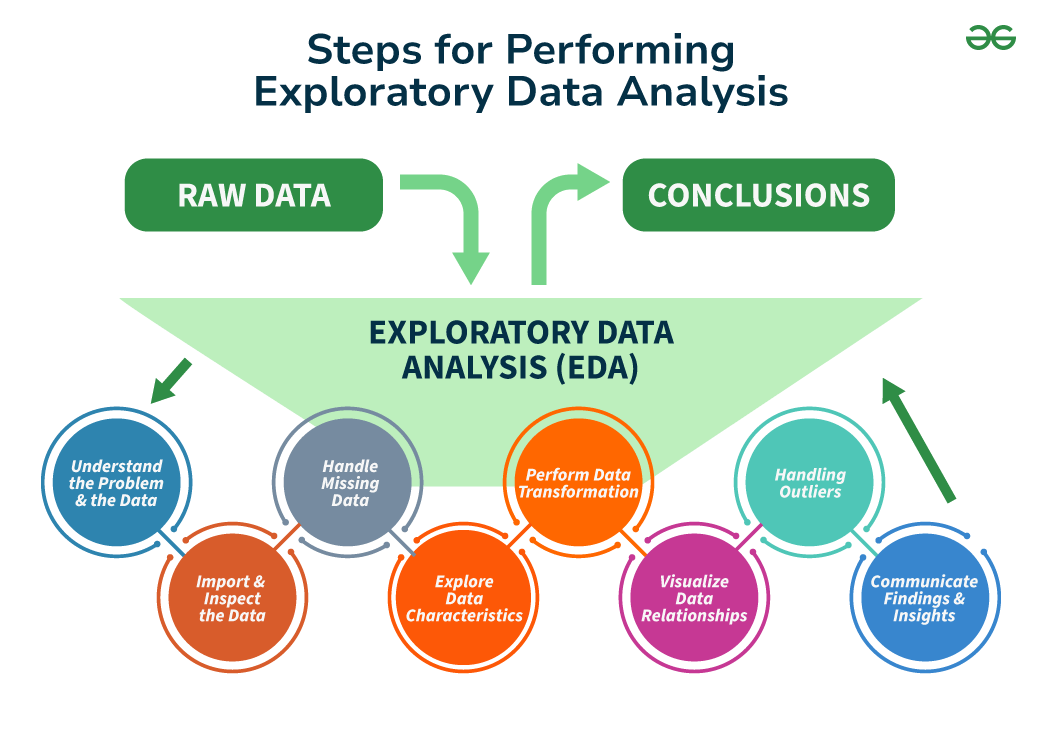
\includegraphics[width=0.6\textwidth]{figures/eda.png}
\caption{Steps of Performing EDA }
\end{figure}
For instance, if we want to explore climate data using Exploratory Data Analysis (EDA), we begin by loading the climate data, such as daily temperatures, into an analysis environment. The first step is to inspect the data for any missing values or errors. Next, we analyze the temperature distribution using histograms to determine whether the weather is mostly warm or cool. We also examine the relationship between temperature and other variables, like humidity, using scatter plots. In more complex cases, we explore how multiple factors, such as temperature, humidity, and wind speed, interact with each other. If we find missing data, we can either remove the affected entries or replace them with average values. Based on our analysis, we might identify trends, like rising temperatures over time, which could suggest climate change. Finally, we use visual tools such as scatter plots and heatmaps to clearly illustrate these relationships and communicate our findings. 
In this book, we will dive deeper into how to analyze climate data using these methods and explore additional techniques to uncover meaningful insights from real-world climate datasets.


\section{R Language for Data Analytics}

R is a widely-used programming language specifically designed for data analytics, statistical computing, and data visualization. It’s an excellent tool for exploring, analyzing, and interpreting complex datasets, making it highly suitable for various fields, including climate data analysis.

R excels in providing an extensive collection of packages and libraries that support tasks like data manipulation, statistical analysis, and generating visualizations. Some popular packages include \texttt{ggplot2} for data visualization, \texttt{dplyr} for data manipulation, and \texttt{tidyverse}, which bundles several powerful tools for data analysis. R is highly favored for its powerful statistical modeling capabilities and its ability to handle large datasets efficiently, which is especially useful when dealing with climate data or similar complex datasets.

The primary development platform for R is RStudio, an Integrated Development Environment (IDE) that provides an intuitive interface for coding, debugging, and visualizing data analysis results. RStudio makes it easier to write and execute R code by organizing the workspace into multiple panes for code writing, console output, and data visualizations. It offers features like code completion, a comprehensive help system, and a history of commands, which boosts productivity and efficiency in data analysis tasks.

Apart from RStudio, there are other platforms like JASP and Google Colab that can be used for data analytics. Google Colab is a cloud-based environment that enables R programming alongside Python. It allows easy access to resources without the need for local setup, making it a great choice for collaborative data science projects. Colab is especially useful for those who want to combine Python and R in a single workflow or need cloud-based resources for large-scale data analysis.

JASP (Jeffrey’s Amazing Statistics Program) is a free, open-source software platform designed for statistical analysis and data visualization. It integrates seamlessly with R, allowing for reproducible research, and is widely used in education and research due to its interactive features and visually appealing outputs. JASP is ideal for users who prefer a more interactive approach to data analysis without heavy reliance on coding, but still want powerful statistical analysis capabilities.

In this book, we will focus on leveraging R for data analytics, with a special emphasis on its applications for analyzing and visualizing climate data. We will explore how platforms like JASP and Google Colab can complement your analysis, making it easier to integrate multiple tools and enhance your analytical capabilities.

\section{Expanding Your R Toolkit with Packages}

Imagine R as a construction site where you’re building a house. The basic R installation gives you the essential tools—like a shovel and a measuring tape—to get started. However, as the project progresses, you need specialized machinery, such as a crane for lifting heavy materials, a cement mixer for mixing concrete, or a laser cutter for precise measurements. In R, packages are those specialized machines: they help you manage more complex tasks, streamline your workflow, and produce better, more accurate results. Without the right package, completing your project efficiently would be a lot harder.

\subsection{What are R Packages?}

An R package is a collection of reusable R functions, documentation that explains how to use them, and often sample data sets, all bundled together. Packages are created by the global R community and allow you to extend R’s capabilities far beyond the basics. Instead of writing complex code from scratch for every task, you can use a package designed specifically for that job.

\subsection{Finding and Using Packages}

Thousands of packages are available from online repositories, the main one being CRAN (The Comprehensive R Archive Network). You typically install a package once using the command:

\begin{verbatim}
install.packages("package name")
\end{verbatim}

Once installed, you need to load the package into your current R session to use its functions. Think of this like taking the specialized tool out of its box and putting it on your workbench. You do this using the command:

\begin{verbatim}
library(package name)
\end{verbatim}

Let’s explore some of the most useful and popular packages you’ll likely encounter. We’ll group them by the kind of tasks they help with.

\subsection{Core Data Science Tools: The tidyverse Ecosystem}

Many modern data analysis workflows in R rely on a collection of packages known as the \texttt{tidyverse}. These packages share a common design philosophy, making them work seamlessly together. Loading the main \texttt{tidyverse} package (\texttt{library(tidyverse)}) gives you access to several key packages at once.

\paragraph{dplyr: The Data Manipulator}

\textbf{What it Does:} Provides a set of core functions (called “verbs”) for the most common data manipulation tasks: subsetting, transforming, rearranging, and summarizing data stored in tables (data frames or tibbles).

\textbf{Why Use It?}
\begin{itemize}
    \item Intuitive Verbs: Functions have simple action-oriented names like \texttt{filter()} (keep rows based on conditions), \texttt{select()} (pick columns by name), \texttt{arrange()} (sort rows), \texttt{mutate()} (create or change columns) and \texttt{summarise()} (calculate summary statistics). This makes your code easy to write and understand.
    \item Readable Workflows: \texttt{dplyr} works beautifully with the pipe operator (\texttt{\%\textgreater\%} or the newer \texttt{|>}). This lets you chain operations together sequentially, making complex data transformations read like a set of instructions (e.g., \texttt{take data \%\textgreater\% then filter rows \%\textgreater\% then select columns}).
    \item Efficiency: Designed to be fast and efficient for most common data sizes you’ll work with directly in R.
    \item Consistency: As part of the tidyverse, it uses consistent rules and structures, making it easier to learn alongside other related packages.
\end{itemize}


\paragraph{ggplot2: The Grammar of Graphics}

\textbf{What it Does:} Implements the “Grammar of Graphics,” allowing you to build plots layer by layer. You start with your data, map variables to visual elements (like axes, colors, shapes), and then add geometric shapes (points, lines, bars, etc.).

\textbf{Why Use It?}
\begin{itemize}
    \item Power \& Flexibility: You can create a vast range of plot types, from simple scatter plots and bar charts to intricate multi-layered visualizations, all using the same core principles.
    \item High-Quality Output: Produces aesthetically pleasing, publication-quality graphics with sensible defaults.
    \item Customization: Offers deep control over every element of the plot.
    \item Logical Structure: Although it takes a little practice, the layered approach (\texttt{ggplot(...) + geom\_point() + labs(...)}) is a logical and consistent way to think about and build plots.
    \item Vibrant Community: Benefits from extensive online documentation, examples, and add-on packages for specialized plots.
\end{itemize}

\paragraph{tidyr: The Data Tidier}

\textbf{What it Does:} Helps you reshape your data into a “tidy” format. Tidy data has a consistent structure (each variable in a column, each observation in a row) that makes it easier to work with in R, especially within the tidyverse. Key functions help you pivot data between “wide” and “long” formats (\texttt{pivot\_wider()}, \texttt{pivot\_longer()}) or split/combine columns (\texttt{separate()}, \texttt{unite()}).

\textbf{Why Use It?}
\begin{itemize}
    \item Simplifies Cleaning: Addresses common messy data layouts, making data preparation much easier.
    \item Essential for tidyverse: Tidy data is the expected format for \texttt{dplyr} and \texttt{ggplot2}, so \texttt{tidyr} is often a crucial first step.
    \item Consistent Syntax: Follows the same design principles as other tidyverse packages.
\end{itemize}

\paragraph{readr: The Data Reader}

\textbf{What it Does:} Provides functions to read rectangular data from delimited text files like CSV (comma-separated values) and TSV (tab-separated values) into R.

\textbf{Why Use It?}
\begin{itemize}
    \item Speed: Often significantly faster than R’s built-in reading functions.
    \item User-Friendly: Gives helpful progress bars for large files and makes smarter guesses about column types.
    \item Modern Output: Reads data into tibbles, a modern type of R data frame used throughout the tidyverse.
    \item Sensible Defaults: Avoids common pitfalls like automatically converting text strings into factor variables.
\end{itemize}

\subsection{High-Performance Data Handling}

\paragraph{data.table: The Speed Demon}

\textbf{What it Does:} Provides an alternative way to work with data tables, optimized for speed and memory efficiency, especially with very large datasets.

\textbf{Why Use It?}
\begin{itemize}
    \item Speed: Can perform subsetting, grouping, joining, and updating operations much faster than dplyr or base R, particularly as data size grows.
    \item Memory Efficient: Uses clever techniques to modify data without making unnecessary copies, saving RAM.
    \item Concise Syntax: Uses a compact \texttt{DT[i, j, by]} syntax that can express complex operations in minimal code.
    \item Great for Big Data: The go-to package if you are pushing the limits of your computer’s memory or need maximum performance.
\end{itemize}

\subsection{Modeling and Machine Learning}

\paragraph{caret: The Modeling Workbench}

\textbf{What it Does:} Offers a unified interface for many tasks involved in machine learning: splitting data, pre-processing features, training various models using different algorithms, tuning model parameters, and evaluating performance.

\textbf{Why Use It?}
\begin{itemize}
    \item Unified Workflow: Provides a consistent set of functions (\texttt{train()}, \texttt{predict()}) to work with hundreds of different modeling techniques from various other R packages. This saves you from learning many different syntaxes.
    \item Streamlines Common Tasks: Simplifies processes like cross-validation, data preparation, and comparing model performance.
    \item Powerful and Feature-Rich: Offers extensive options for tuning and evaluating models.
\end{itemize}

\subsection{Specialized Utility Packages}

\paragraph{lubridate: The Date/Time Specialist}

\textbf{What it Does:} Simplifies working with date and time data, which can often be tricky. It provides easy functions for parsing dates/times from text, extracting components (like year, month, day, weekday), and doing calculations involving time.

\textbf{Why Use It?}
\begin{itemize}
    \item Intuitive Functions: Has memorable function names (e.g., \texttt{ymd()} to parse YearMonth-Day formats, \texttt{year()} to extract the year, \texttt{now()} to get the current time).
    \item Handles Complexity: Makes dealing with different formats, time zones, and date arithmetic much less error-prone than using base R functions alone.
    \item Essential for Time Series: Indispensable if your data involves timestamps or time-based analysis.
\end{itemize}

\paragraph{stringr: The Text Wrangler}

\textbf{What it Does:} Offers a consistent and simplified set of functions for common text manipulation tasks, such as detecting patterns (\texttt{str\_detect()}), replacing text (\texttt{str\_replace()}), splitting text into pieces (\texttt{str\_split()}), extracting parts of text (\texttt{str\_extract()}), and joining text together (\texttt{str\_c()}, \texttt{str\_glue()}).

\textbf{Why Use It?}
\begin{itemize}
    \item Consistency: Provides a cleaner, more predictable interface compared to base R’s string functions.
    \item Easier Regular Expressions: Simplifies the use of regular expressions (powerful pattern matching codes) for complex text tasks.
    \item tidyverse Friendly: Works well with the pipe operator and other tidyverse tools, making it great for cleaning text data within a larger workflow.
\end{itemize}

This list only scratches the surface! The beauty of R lies in this vast package ecosystem. As you encounter new tasks, chances are there’s a package out there designed to help. Don’t hesitate to search CRAN, read package documentation, and explore vignettes (package tutorials) to expand your R toolkit.
\chapter{Preparing Climate Data with R in Colab}

Welcome to the practical side of data analysis! In Chapter 1, we explored the power of R packages. Now, we’ll apply that knowledge to a real-world scenario: working with climate data. Climate data, like weather station readings (temperature, precipitation, etc.), is fascinating but often comes with imperfections. It might have missing measurements, incorrect values, or inconsistent formats.

Before we can analyze data and draw meaningful conclusions, we must clean and preprocess it. This means identifying and fixing errors, handling missing information, and transforming the data into a suitable format for analysis. Think of it like preparing your ingredients before cooking – essential for a good final result!

In this chapter, we’ll use Google Colaboratory (Colab), a free, cloud-based platform that lets you write and run code (including R!) directly in your web browser. This is fantastic because you don’t need to install complex software on your own computer, and you can easily save and share your work.

\section{Setting Up Your Colab Environment for R}

Google Colab primarily supports Python, but we can easily configure it to run R code. To set up R environment we can perform following steps:

\begin{enumerate}
    \item \textbf{Access Google Colab:} Open your web browser and go to \url{https://colab.research.google.com}. You’ll need a Google account to use it.
    \item \textbf{Create a New Notebook:} Click on \texttt{File} $\rightarrow$ \texttt{New notebook}. This creates a new, empty Colab notebook file (which is automatically saved to your Google Drive). Rename it something descriptive, like ``Climate Dataset Analysis.''
    \item \textbf{Understanding the Interface:}
    \begin{itemize}
        \item \textbf{Cells:} Colab notebooks are made of cells. You’ll use Code cells to write and run R code and Text cells to add notes and explanations using Markdown.
        \item \textbf{Runtime:} This is the virtual machine in the cloud running your code.
        \item \textbf{Running Cells:} To run a cell, click the play button to its left or press \texttt{Shift + Enter}.
    \end{itemize}
    \item \textbf{Change Runtime to R:}
    \begin{itemize}
        \item Click \texttt{Runtime} on the menu.
        \item Choose \texttt{Change runtime type}.
        \item In the dropdown under ``Language,'' select \texttt{R}.
        \item Click \texttt{Save}.
    \end{itemize}
    \item \textbf{Installing Packages:} As shown in the setup cell, you install R packages in Colab just like you would locally, using \texttt{install.packages("package name")}. Any packages you install will be available for your current session but might need reinstalling if the runtime fully resets after a long period of inactivity.
\end{enumerate}

\section{Getting Climate Data into Colab}

Now we need some reliable data to conduct meaningful analysis. In this chapter, we will work with climate data from Nepal, covering the period from 1980 to 2019. This dataset includes important environmental indicators such as temperature, precipitation, and humidity, which will help us explore climate trends over time.

\subsection*{Where to Find Climate Data:}

The dataset used in this chapter is publicly available on the Kaggle platform, a popular repository for datasets and data science projects. The dataset contains climate data for Nepal, including various meteorological parameters. These data were sourced from the NASA Langley Research Center (LaRC) POWER Project, which is funded through the NASA Earth Science/Applied Science Program. The data was extracted via NASA’s Power Access API. The information is based on measurements from 93 weather stations across 62 districts in Nepal, providing a comprehensive view of the country’s climate. We will import the required dataset directly from Kaggle. Make sure you have a Kaggle account.

You can view or download the dataset using the following link:

\medskip

\href{https://www.kaggle.com/code/saimondahal/nepal-climate-data-eda-insights/input}{Click here to access the dataset on Kaggle
}
\medskip

\subsection*{Loading Dataset in Colab:}

The dataset that we downloaded is in \texttt{.csv} format. We can rename the downloaded dataset as \texttt{dailyclimate.csv}. There are many ways to load the dataset in the Colab environment.
\begin{enumerate}
\item {Uploading Directly (Best for small files, $<$ 25MB)}  
    \begin{itemize}
        \item Click the folder icon in the left sidebar of Colab.
        \item Click the ``Upload'' button.
        \item Select your \texttt{weather data raw.csv} file from your computer.
    \end{itemize}
\noindent \textit{Note: Files uploaded this way disappear when the runtime restarts.}

\item {Mounting Google Drive (Recommended for larger/persistent files)}  
For this you must have the \texttt{dailyclimate.csv} in your Google Drive. Place your \texttt{dailyclimate.csv} file somewhere convenient in your Google Drive (e.g., in a folder called \texttt{Colab Data}).

    \begin{itemize}
        \item Click the folder icon in the left sidebar.
        \item Click the ``Mount Drive'' button (looks like a Google Drive logo).
        \item Follow the prompts in the popup window and the new code cell that appears. You’ll need to authorize Colab to access your Google Drive.
        \item Once mounted, your Google Drive files will appear under \texttt{/content/drive/MyDrive/}. You can navigate this like any other folder system.
    \end{itemize}
\end{enumerate}
We have successfully loaded the dataset in our Colab environment and now we can begin our data preparation for analysis.

\section{First Look - Exploring Your Climate Data}

Before cleaning, we need to understand our raw data. What does it look like? What kind of information does it contain? Are there obvious problems?

\subsection{Loading the Data into R}

Assuming you have the file available (either uploaded or on Drive), load it using \texttt{readr} (part of the tidyverse).

\begin{verbatim}
library(tidyverse)

# Path if mounted on Google Drive:
file_path <- "/content/drive/MyDrive/Colab_Data/dailyclimate.csv"

# Load the data
climate_data <- read.csv(file_path)

# Quick check
head(climate_data) # Display the first 6 rows
\end{verbatim}

\subsection{Dataset Dimension}

\begin{verbatim}
dim(climate_data)
\end{verbatim}
Dimension: 883,128 rows $\times$ 23 columns.

The dataset has 883,128 rows and 23 columns.

\subsection{Dataset Structure}

Understanding the structure of the dataset is essential before proceeding to cleaning. In R, we can use the below function to inspect the dataset.

\begin{verbatim}
str(climate_data)
\end{verbatim}

% Figure here ----------------------------
\begin{figure}[h!]
    \centering
    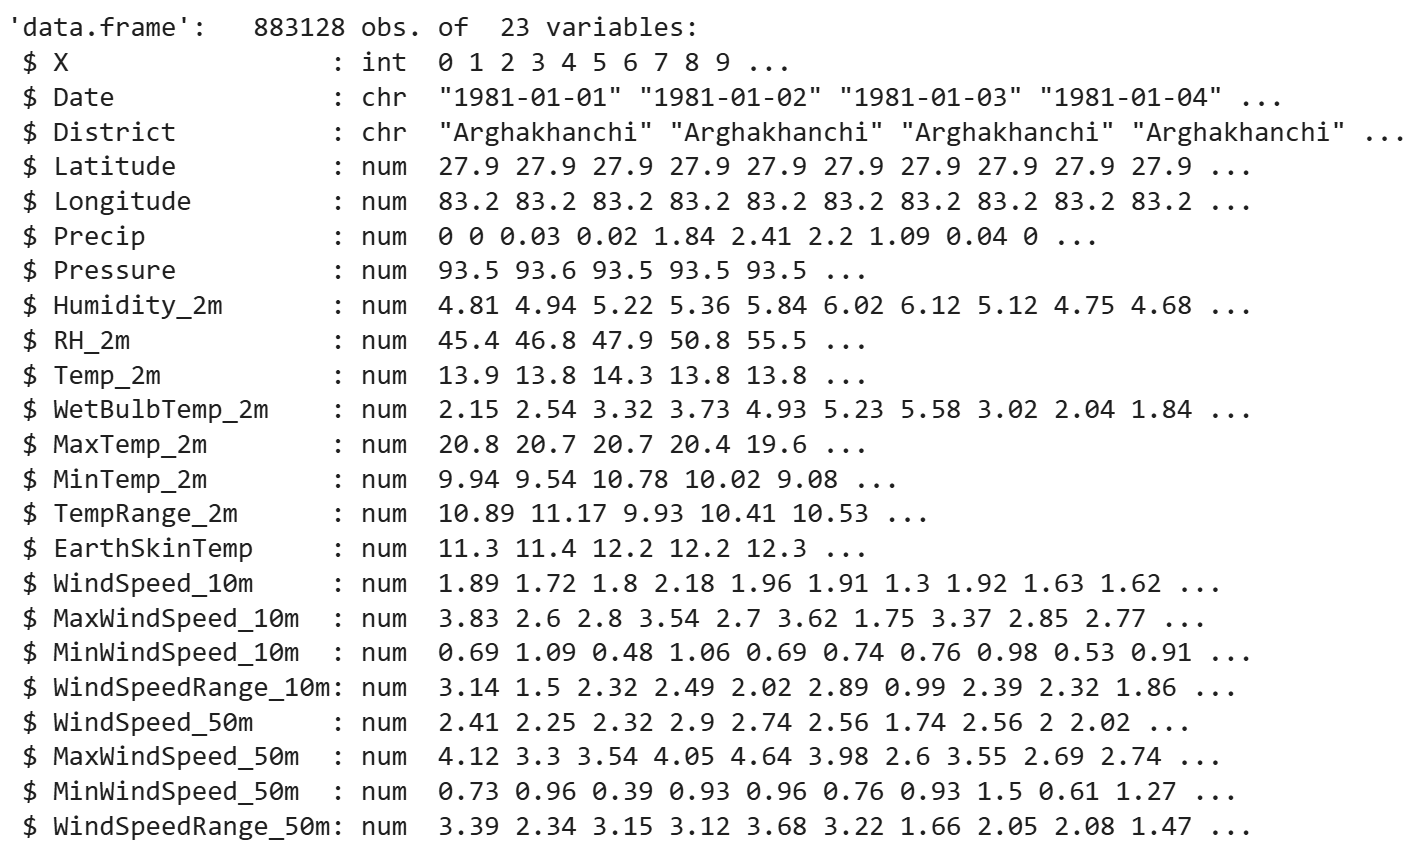
\includegraphics[width=0.7\textwidth]{figures/raw.png}
    \caption{Structure of the Climate Dataset.}
\end{figure}

\subsection{Data Summary}

The \texttt{summary()} function in R provides a quick statistical summary of each column in the dataset. It includes descriptive statistics like mean, median, minimum, maximum, and quartiles. It also shows missing values (NA) and category counts for factors.

\begin{verbatim}
summary(climate_data)
\end{verbatim}

% Figure here----------------------------
\begin{figure}[h!]
    \centering
     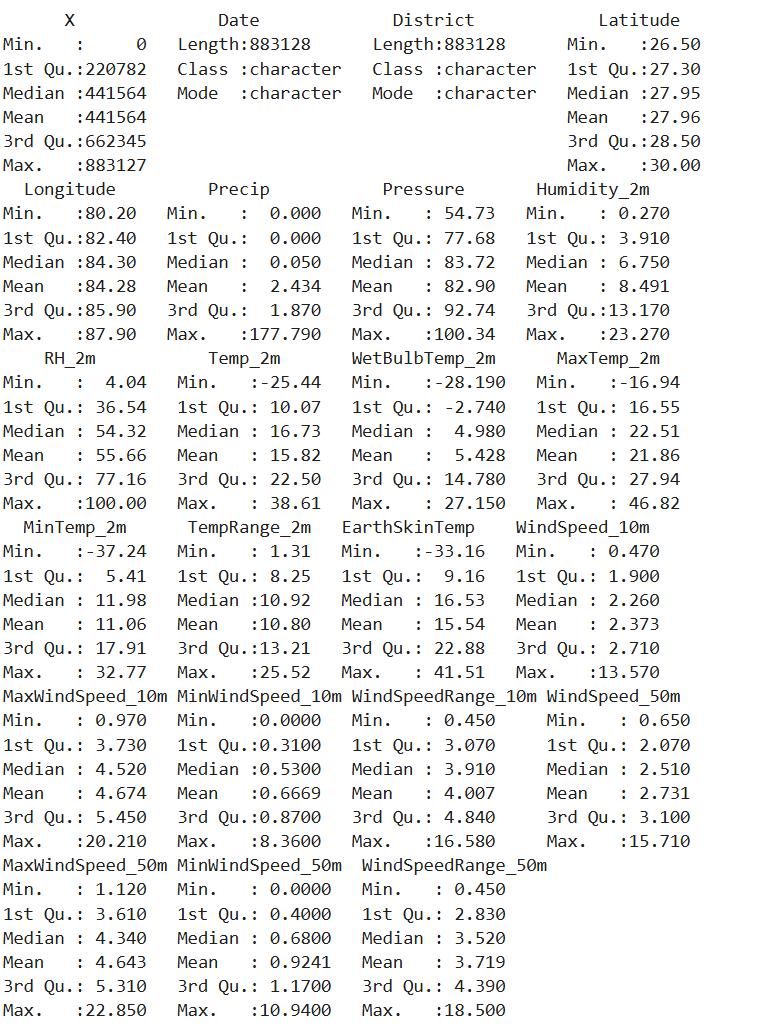
\includegraphics[width=0.5\textwidth]{figures/summary.png}
    \caption{Summary of the Climate Dataset.}
\end{figure}

\subsubsection*{What to Look for During Exploration:}

\begin{enumerate}
    \item \textbf{Data Types:} Are dates recognized as dates? Are numeric values (like temperature) stored as numbers or text?
    \item \textbf{Missing Values (NA):} How many missing values are there in each column (\texttt{summary()} is great for this)?
    \item \textbf{Ranges:} Do minimum and maximum values make sense (\texttt{summary()})? (e.g., Temperatures shouldn’t be -200°C, precipitation shouldn’t be negative).
\end{enumerate}

\section{Data Preprocessing}

Data preprocessing is the process of preparing raw data for analysis by cleaning and transforming it into a usable format. In data mining it refers to preparing raw data for mining by performing tasks like cleaning, transforming, and organizing it into a format suitable for mining algorithms.

Goal is to improve the quality of the data, handling missing values, removing duplicates, and normalizing data to ensures the accuracy and consistency of the dataset.

\subsection{Data Cleaning}

In this step, we focus on cleaning the dataset to prepare it for analysis.

\begin{enumerate}
\item \textbf{Check For Null Values:}

We should identify any missing values across the dataset, and decide how to handle them (impute, drop, or analyze separately). For this particular dataset no null values were found.

\begin{verbatim}
sum(is.na(df_climate))
\end{verbatim}

\item\textbf{Drop the unnecessary columns:}

In our data set the first column consisting of an index is not necessary so we can drop the first unnamed column from our climate dataset.

\begin{verbatim}
df_climate$X <- NULL
\end{verbatim}

\item\textbf{Inspect the Duplicate Columns:}

We must also check for duplicate columns and remove them as they don't provide any additional information. For this particular climate dataset no such columns were found.

\begin{verbatim}
duplicated(colnames(df_climate))
\end{verbatim}

\item\textbf{Convert Date Column to Date Format:}

Since the Date column is currently in character format, convert it to Date using \texttt{as.Date()}.

\begin{verbatim}
df_climate$Date <- as.Date(df_climate$Date, format = "%Y-%m-%d")
\end{verbatim}

\item \textbf{Set Date as Index:}

Setting the date as an index is not strictly necessary in R for time series data analysis, but it is often a good practice and can simplify time-based operations. Setting the date as an index (or primary column) helps in slicing, filtering, and aggregating data by time periods. For this data set I used \texttt{tsibble} package.

\begin{verbatim}
# Convert tibble to tsibble
df_climate <- as_tsibble(df_climate, index = Date, key = District)

# Check for index
index_name <- index_var(df_climate)
print(index_name)
\end{verbatim}

The dataset structure after cleaning looks like:

\begin{verbatim}
glimpse(df_climate)
\end{verbatim}

% Figure here ---------------------------
\begin{figure}[h!]
    \centering
    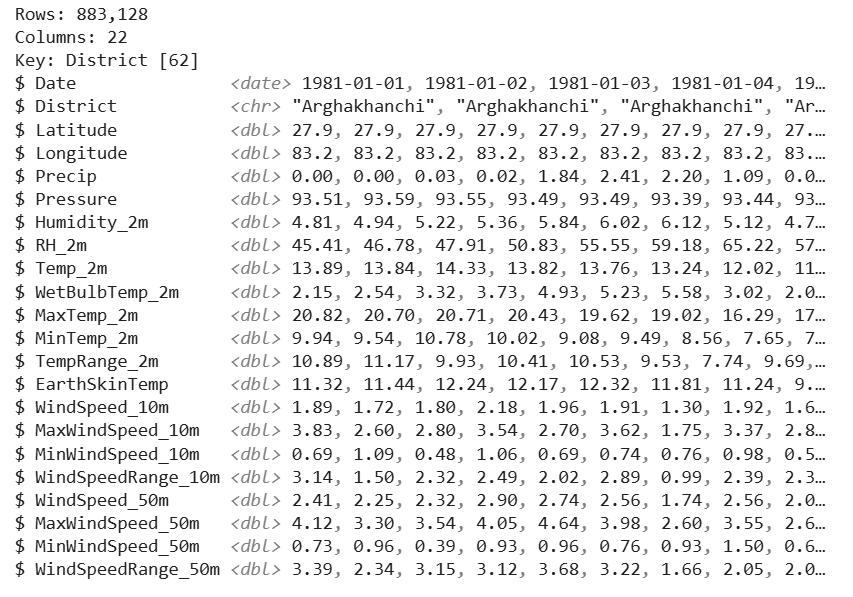
\includegraphics[width=0.6\textwidth]{figures/glimpse.png}
    \caption{Glimpse of the Cleaned Climate Dataset.}
\end{figure}

\end{enumerate}
\subsection{Feature Engineering}

Feature engineering is the process of taking raw data and transforming it into meaningful inputs that help a machine learning model understand patterns better. Think of it like preparing ingredients before cooking like when you chop, mix, and season them so the final dish tastes great.

In data analysis, this means creating new variables, cleaning data, selecting important information, or combining features to improve the model’s ability to make accurate predictions. Good feature engineering can often make a bigger difference in model performance than just using more complex algorithms.

It helps to create new features that might be helpful for your analysis. For this dataset, we can derive the month column from Date. Since Date is in format YYYY-MM-DD, we can extract the month and create a new column called month number. We can also create another column called month label and assign the names of the month (e.g., 1 = Jan, 2 = Feb, and so on).

\begin{verbatim}
# Extract month as number and label
df_climate$Month_Number <- month(df_climate$Date)     
df_climate$Month_Label <- month(df_climate$Date, label = TRUE)
\end{verbatim}

We can categorize the months into season and create a new column called “Season” for seasonal data analysis in the following way:

\begin{verbatim}
# Categorize months into seasons
df_climate <- df_climate %>%
  mutate(Season = case_when(
    month(Date) %in% c(12, 1, 2)  ~ "Winter",
    month(Date) %in% c(3, 4, 5)   ~ "Spring",
    month(Date) %in% c(6, 7, 8)   ~ "Summer",
    month(Date) %in% c(9, 10, 11) ~ "Fall"
  ))
\end{verbatim}

In R we can use \texttt{dplyr} and \texttt{lubridate} to extract the components of date. The function called \texttt{mutate()} can be used for creation of new columns and modifying the existing columns in our case.

\chapter{Unveiling Insights: Visualizing and Exploring Data with R}

Now, when it comes to the specific task of creating blueprints and visual representations of our house things like floor plans, elevation drawings, or even a 3D model. We need specialized architectural software designed for this purpose.

In the R world, the equivalent of this architectural software for creating stunning and informative visualizations is the \texttt{ggplot2} package.
 \section{Histogram: Seeing the Shape of Your Numbers}

Imagine you’re organizing a large set of test scores from a group of students. You want to see how the scores are distributed: Are most students scoring in the 80s, or is there a wider spread?

A histogram is like a map of all the test scores, showing you where the majority of students are scoring and how the scores spread out across different ranges.

\subsection*{Key Concepts: Let’s Explore!}

\textbf{Numerical Data: Numbers are Key!}

Numerical data can represent things like: 
\begin{itemize}
    \item Test scores
    \item The amount of time spent studying
    \item The number of goals scored in a match
\end{itemize}

\textit{Activity: Can you think of three other examples of numerical data you use regularly?}

Histograms are specifically for numerical data. Why do you think histograms are used for numbers and not for things like colors or types of fruit? (Hint: Numbers have an inherent order, and you can compare them to each other more easily.) \newline

\noindent\textbf{Bins (Intervals): Grouping for Clarity}

Imagine breaking the range of test scores [0,100] into bins, or groups. For example, one bin might represent scores from 0 to 10, another from 11 to 20, and so on. These bins help us organize the data into manageable chunks. \newline

\textit{Activity: Why do you think we group the data into bins? What would happen if we had a “bin” for every single score, especially with a large number of students?} (Hint: If you have too many bins, it can be hard to see the patterns clearly.) \newline

Why do you think it’s better to keep the width of each bin the same? (Hint: Consistent bin widths make the histogram easier to read and compare.) \newline

\noindent\textbf{Frequency: Counting What Falls Where}

Once we’ve grouped the scores into bins, we count how many students fall into each range. This is called frequency. For example:
\begin{itemize}
    \item 5 students scored between 0–10,
    \item 12 students scored between 11–20,
    \item 10 students scored between 21–30.
\end{itemize}

\textit{Activity: If you have more students in one bin than another, what does this tell you about the scores in that range?} \newline

\noindent\textbf{Bars: Visualizing the Counts}

We then draw a bar for each bin, where the height of the bar represents the frequency (how many students scored in that range). \newline

\textit{Activity: If one bar is much taller than another, what does this mean?} (Hint: A taller bar shows a higher frequency, meaning more students scored in that range.)\newline

\noindent\textbf{Shape of Distribution: Unveiling Patterns}

The overall shape of the histogram reveals key insights about the distribution of the data. Let’s look at some common shapes:

\begin{itemize}
    \item \textbf{Symmetry or Skewness:}
    \begin{itemize}
        \item \textit{Symmetric:} Imagine the histogram looks like a bell curve (a normal distribution). This suggests the data is evenly distributed, with most students scoring around the middle.
        \item \textit{Skewed:} What if the histogram is lopsided, with a long tail on one side? Skewed data often has outliers that pull the data to one side, such as a few students with very high or very low scores.
    \end{itemize}
    \item \textbf{Central Tendency:} The center of the histogram (where the highest bars are) gives us a sense of where most of the data lies. The center is often close to the average, or mean, of the data.
    \item \textbf{Spread or Variability:} A wide histogram with bars spread across many bins suggests that the data has a wide range of values. A narrow histogram shows the data is concentrated around one main value.
    \item \textbf{Modality:}
    \begin{itemize}
        \item \textit{Unimodal:} A histogram with one peak suggests that most data points group around one central value.
        \item \textit{Bimodal:} A histogram with two peaks suggests two distinct groups in the data.
    \end{itemize}
\end{itemize}

\textit{Activity: Can you think of a situation where a bimodal distribution might occur?} (Hint: If you have data from two groups, like the test scores of two different classes with very different performance levels, you might see two peaks.)

Now let’s explore the climate dataset and visualize histogram using R.

\subsection*{Pressure Distribution using Histogram}

\begin{verbatim}
histogram(~ Pressure, df_climate,
          main = "Distribution of Atmospheric Pressure",
          xlab = "Pressure (hPa)",
          ylab = "Frequency",
          breaks = 30)
\end{verbatim}

% Figure here -------------------------
\begin{figure}[h!]
    \centering
     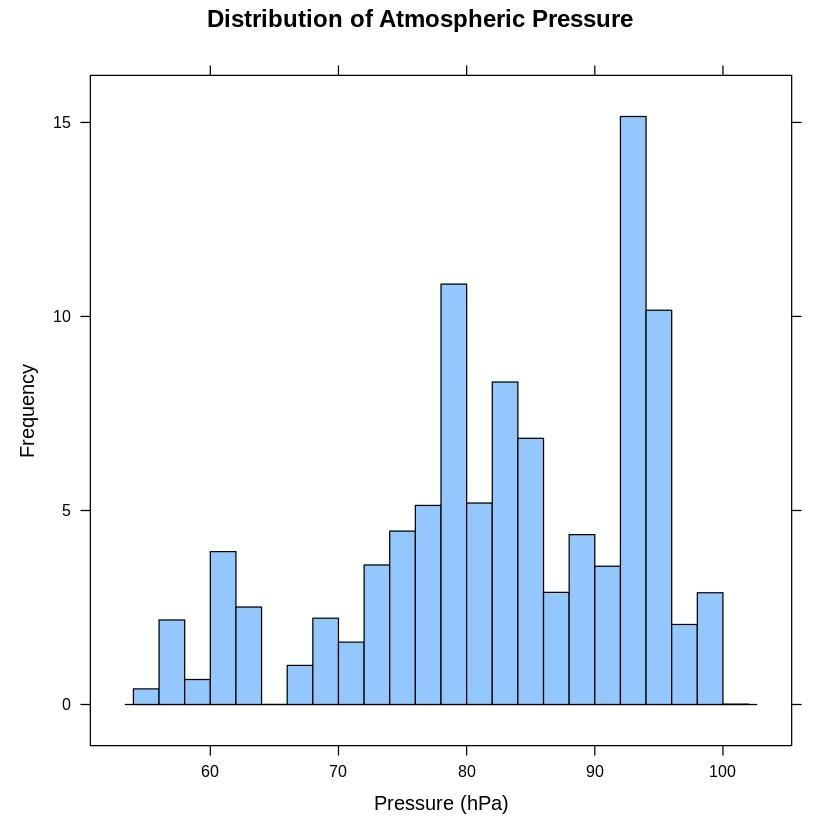
\includegraphics[width=0.6\textwidth]{figures/hist1.jpg}
    \caption{Pressure Distribution using histogram}
\end{figure}


\subsection*{Wind Speed Distribution Analysis with Density Curve}

\begin{verbatim}
# Create histogram with density curve
ggplot(df_climate, aes(x = WindSpeed_10m)) +
  geom_histogram(aes(y = after_stat(density)), bins = 30, 
  fill = "skyblue", color = "black", alpha = 0.7) + 
  geom_density(color = "blue", linewidth = 1) + 
  labs(title = "Histogram of Windspeed with Density Trendline ",
       x = "Temperature (°C)",
       y = "Density") +
  theme_minimal()
\end{verbatim}

% Figure here --------------------------
\begin{figure}[h!]
    \centering
     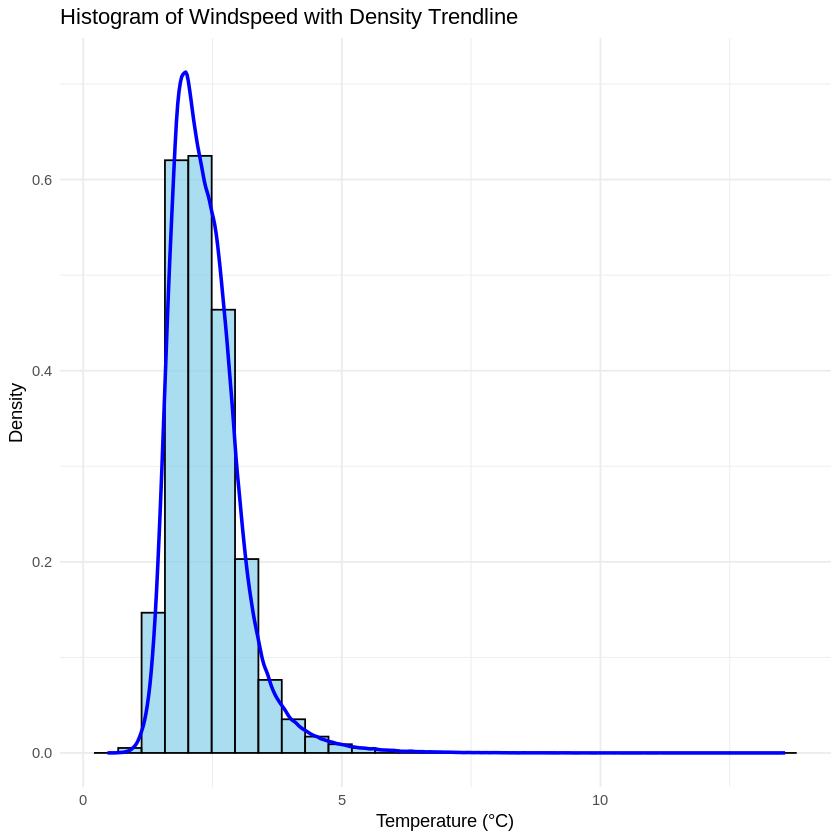
\includegraphics[width=0.5\textwidth]{figures/hist2.png}
    \caption{ Windspeed with Density Trend}
\end{figure}

 \section{Scatter Plot: Discovering Relationships Between Two Variables}

A scatter plot is a type of graph that shows the relationship between two numerical variables. Each point on the plot represents one observation in your data, defined by its values on two axes.

\subsection*{Key Concepts: Let’s Explore}

\begin{enumerate}
    \item \textbf{Two Variables: X and Y} \\
    Think about situations where two quantities vary together:
    \begin{itemize}
        \item Hours studied vs. test scores
        \item Height vs. weight
        \item Temperature vs. ice cream sales
    \end{itemize}
    Can you think of three more examples where one thing might change as another?

    \item \textbf{Each Point = One Observation} \\
    In a scatter plot, each dot represents one observation from your dataset. Its position is determined by:
    \begin{itemize}
        \item Its value on the x-axis (horizontal)
        \item Its value on the y-axis (vertical)
    \end{itemize}

    \item \textbf{Patterns: Relationships or Trends} \\
    Scatter plots help us see relationships between variables:
    \begin{itemize}
        \item Positive relationship: As X increases, Y tends to increase
        \item Negative relationship: As X increases, Y tends to decrease
        \item No clear relationship: The points appear scattered
    \end{itemize}
    If your plot shows points climbing upwards, what might that suggest?

    \item \textbf{Clusters, Outliers, and Spread} \\
    Scatter plots also reveal:
    \begin{itemize}
        \item Clusters: Groups of similar points 
        \item Outliers: Distant or unusual points
        \item Spread: How widely points are distributed
    \end{itemize}

    \item \textbf{Line of Best Fit (Trend Line)} \\
    Sometimes we add a trend line (or regression line) to summarize the general direction of the relationship.
\end{enumerate}

\subsection*{Let’s Try This!}

We have our daily climate dataset. We want to explore how the Humidity and Temperature vary. We can observe this relation with scatter plots.

\paragraph{Relation between humidity and temperature above 2m}

\begin{verbatim}
xyplot(Humidity_2m ~ Temp_2m, data = df_climate,
       main = "Humidity vs. Temperature" ,xlab = "Temperature (°C)",
       ylab = "Humidity (%)", col = "blue",
       panel = function(x, y) {panel.xyplot(x, y)
           panel.abline(lm(y ~ x), col = "red", lwd = 2) #linear trend line
       })  # point color
\end{verbatim}

% Figure here -------------------------
\begin{figure}[h]
\centering
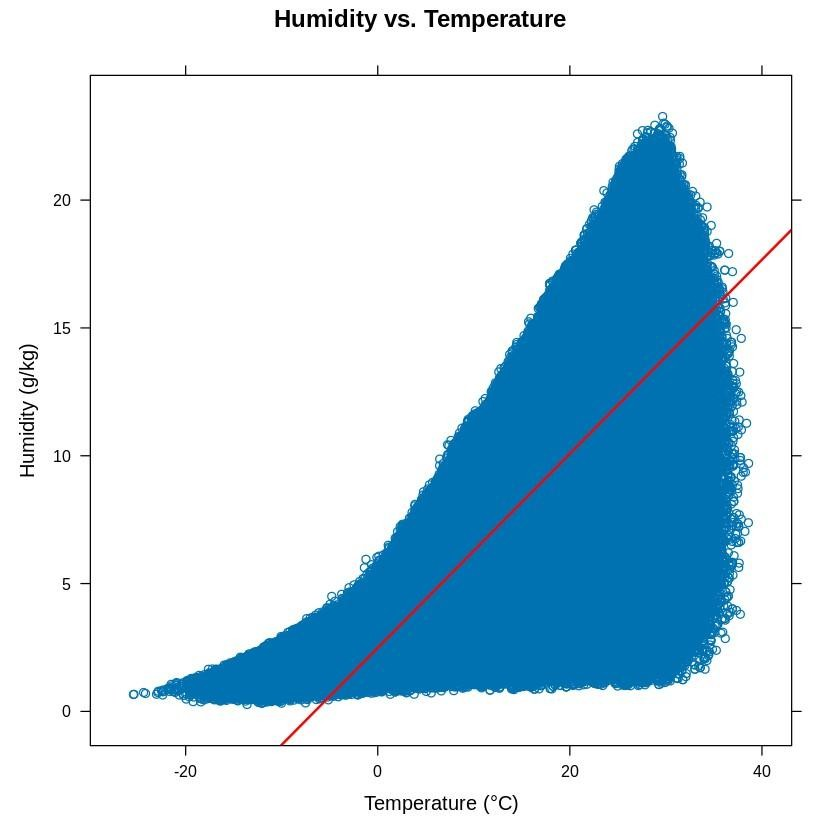
\includegraphics[width=0.5\textwidth]{figures/scatter1.jpg}
\caption{Humidity vs Temperature}
\end{figure}

\subsection*{Analyzing the Relationship Between Wind Speed and Precipitation}

To explore how wind speed at 10 meters (WindSpeed\_10m) relates to precipitation levels (Precip), we use a scatter plot.

\paragraph{Why a Scatter Plot?}

A scatter plot is a two-dimensional graph that displays individual data points for two variables. It helps us see:
\begin{itemize}
    \item Whether there is a relationship or trend between the two variables.
    \item The direction of the relationship (positive, negative, or none).
    \item How closely the points follow a pattern (correlation).
\end{itemize}

In our case, each point represents a day (or observation) with its wind speed on the x-axis and precipitation amount on the y-axis.

\paragraph{R Code: Creating a Scatter Plot with a Trend Line}

\begin{verbatim}
ggplot(climate_data, aes(x = WindSpeed_10m, y = Precip)) +
  geom_point(color = "blue") +
  geom_smooth(method = "lm", color = "red", se = FALSE) +
  labs(title = "Relationship Between Wind Speed and Precipitation",
       x = "Wind Speed (km/h)", y = "Precipitation (mm)") +
  theme_minimal()
\end{verbatim}

% Figure here--------------------------
\begin{figure}[h]
\centering
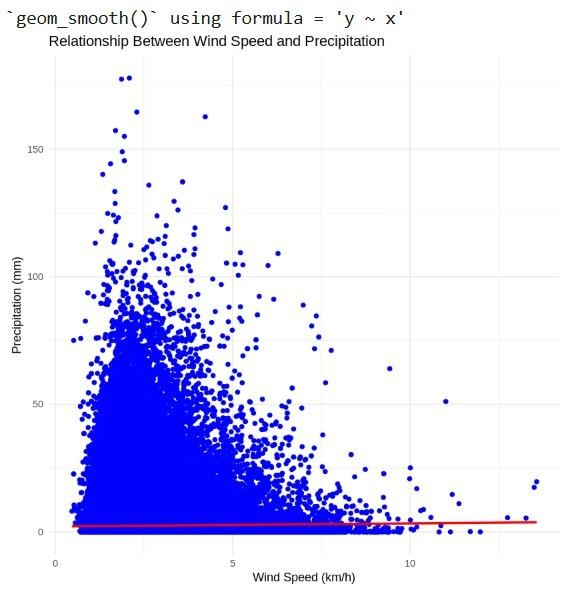
\includegraphics[width=0.5\textwidth]{figures/scatter2.jpg}
\caption{Wind Speed vs Precipitation}
\end{figure}

\paragraph{Explanation:}
\begin{itemize}
    \item \texttt{geom\_point()}: Plots each data point (blue dots).
    \item \texttt{geom\_smooth(method = "lm")}: Adds a red trend line using linear regression.
    \item \texttt{labs()}: Sets the title and axis labels for clarity.
    \item \texttt{theme\_minimal()}: Uses a clean, minimal background.
\end{itemize}

\paragraph{Interpretation:} 

If the red line slopes upward, it indicates that wind speed tends to increase as precipitation increases (a positive relationship). If the slope is downward, it indicates a negative relationship. A flat line suggests no clear relationship between the two variables.

\textit{Activity: Look at the scatter plot—do the points follow a clear upward or downward trend? Are they tightly clustered around the line, or widely scattered? What does this tell you about how wind and rain might interact in this climate?}

 \section{Bar Chart: Comparing Climate Categories Visually}

Imagine you’re studying monthly rainfall data and you want to see which months receive the most and least precipitation. A bar chart is a powerful way to make these comparisons quickly and clearly.

A bar chart displays data using rectangular bars. Each bar represents a category, and its height (or length) shows the value for that category — such as rainfall amount or average temperature.

\subsection*{Key Concepts: Let’s Explore!}

\paragraph{Categorical Data: Comparing Groups} Bar charts are great for visualizing categorical data. In climate studies, this might include:
\begin{itemize}
  \item Rainfall by month
  \item Number of rainy days by season
  \item Average wind speed in different regions
\end{itemize}
\textit{Activity: Can you list three examples of climate-related categories that could be compared using a bar chart?}

\subsubsection*{Bars: Showing Values Clearly} Each bar corresponds to a category (e.g., a month). The taller the bar, the higher the value. The bars are typically spaced apart so you can easily distinguish each category.

\textit{Activity: What does it mean if one bar is twice as tall as another? What if two bars are the same height?}

\subsubsection*{Orientation and Style} Bars can be displayed vertically or horizontally. You can also color them differently to highlight patterns or categories.

\subsubsection*{Grouped Bar Charts:} You can even place bars side-by-side for each category to compare sub-groups (e.g., rainfall in two cities across the same months).

\paragraph{What Can You Learn from a Bar Chart?}
\begin{itemize}
  \item Trends: You can easily see which categories stand out (e.g., the wettest month).
  \item Patterns: You may discover regular patterns, such as increasing rainfall in monsoon months.
  \item Outliers: A very short or tall bar might indicate an unusual value — maybe an outlier.
\end{itemize}

\subsubsection*{Wrap-Up} 
 Bar charts are an essential tool in climate data analysis. They help you:
\begin{itemize}
  \item Compare values across categories
  \item Spot trends and anomalies
  \item Communicate findings clearly
\end{itemize}

Use them when you want to answer questions like: “Which month gets the most rainfall?” or “How does temperature vary by region?”

\subsection*{Comparing Monthly Averages: Humidity vs. Precipitation}

Climate patterns often vary by month, especially when it comes to humidity and precipitation. To understand these monthly trends side by side, a grouped bar chart is a perfect tool. It allows us to visually compare how two climate parameters change together throughout the year.

\paragraph{What is a Grouped Bar Chart?} A grouped bar chart displays bars side-by-side for each category (month in this case). This setup makes it easy to compare two or more measurements — like average humidity and average precipitation — for each month.

\paragraph{Why Use a Bar Chart Here?}
\begin{itemize}
  \item Clear Comparison: Bars side-by-side show how humidity and precipitation levels differ or align each month.
  \item Category-Based Analysis: Perfect for monthly comparisons across a calendar year.
  \item Color Distinction: Using different colors for humidity and precipitation improves visual clarity.
\end{itemize}

\paragraph{R Code for Grouped Bar Chart}

\begin{verbatim}
climate_data$Month_Num <- month(climate_data$Date)
climate_data$Month <- month(climate_data$Date, label = TRUE)
climate_data$Year <- year(climate_data$Date)

monthly_summary <- climate_data %>%
  group_by(Month) %>%
  summarise(
    avg_temp = mean(Temp_2m, na.rm = FALSE),
    avg_humidity = mean(Humidity_2m, na.rm = FALSE),
    avg_precip = mean(Precip, na.rm = FALSE)
  )

data_matrix <- rbind
(monthly_summary$avg_humidity, monthly_summary$avg_precip)
barplot(
  data_matrix,
  beside = TRUE,
  legend.text = c("Average Humidity", "Precipitation"),
  col = c("orange", "cyan"),
  xlab = "Month",
  ylab = "Values",
  names.arg = monthly_summary$Month
)
axis(2, at = seq(0, 20, by = 1))
grid()
\end{verbatim}

% Figure here ---------------------------
\begin{figure}[h]
\centering
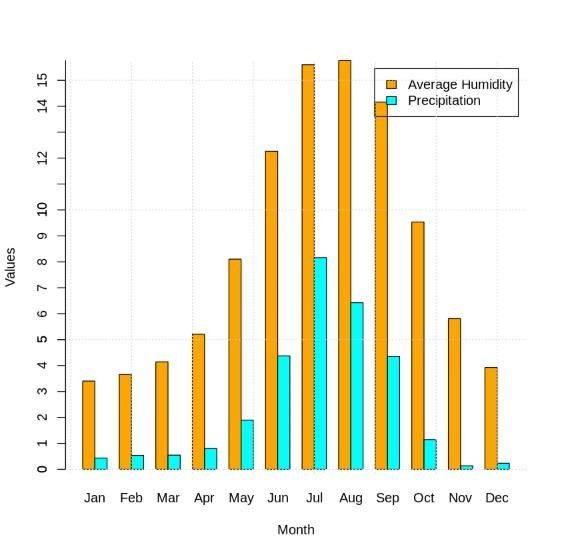
\includegraphics[width=0.6\textwidth]{figures/barchart3.jpg}
\caption{Comparing Monthly Averages: Humidity vs. Precipitation}
\label{fig:monthly_avg_bar}
\end{figure}

\paragraph{How to Interpret This Plot} Each pair of bars corresponds to a month:
\begin{itemize}
  \item Orange bar: Average humidity (\%)
  \item Cyan bar: Average precipitation (mm)
\end{itemize}

\paragraph{Interactive Questions:}
\begin{enumerate}
  \item In which month do humidity and precipitation both peak?
  \item Are there any months where humidity is high but precipitation is low?
  \item What might cause humidity to remain high even when there is little rainfall?
\end{enumerate}

\subsection*{Monthly Extremes: Hottest Month and Driest Month}

Climate extremes help us understand the variability and potential anomalies across the year. In this section, we identify:
\begin{itemize}
  \item The month with the highest average temperature.
  \item The month with the lowest average precipitation.
\end{itemize}

These extremes are valuable for seasonal planning, climate pattern analysis, and risk management.

\paragraph{Step-by-Step Approach}

We used the monthly summary data, already grouped by month, to identify these extremes.

\begin{verbatim}
highest_temp <- monthly_summary[which.max(monthly_summary$avg_temp), ]
lowest_temp <- monthly_summary[which.min(monthly_summary$avg_precip), ]

highest_temp
lowest_temp
\end{verbatim}

% Figure here----------------------------
\begin{figure}[h]
\centering
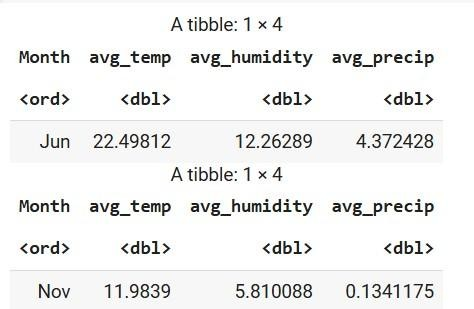
\includegraphics[width=0.5\textwidth]{figures/temp_highlow.jpg}
\caption{Month with Lowest and Highest Temperature}
\label{fig:extremes}
\end{figure}

\subsubsection*{Visualization Using ggplot2 and gridExtra}

The plots below visually highlight these extremes:  
Bar Plot for Temperature: Shows average monthly temperatures, with the hottest month labeled.  
Line Plot for Precipitation: Shows average monthly precipitation, with the driest month labeled.

\paragraph{R Code for Dual Plot Visualization:}

\begin{verbatim}
install.packages("gridExtra")
library(gridExtra)

p1 <- ggplot(monthly_summary, aes(x = as.factor(Month), y = avg_temp)) +
geom_bar(stat = "identity", fill = "red", alpha = 0.5) +
labs(title = "Monthly Temperature", x = "Month", 
y = "Temperature (°C)") +
geom_text(aes(label = ifelse(avg_temp == highest_temp$avg_temp,
paste("Max:", avg_temp, "°C"), "")),
vjust = -0.5, color = "black") +
theme_minimal()

p2 <- ggplot(monthly_summary, aes(x = as.factor(Month), y = avg_precip)) +
geom_line(group = 1) +
geom_point() +
labs(title = "Average Monthly Precipitation", x = "Month", 
y = "Precipitation") +
geom_text(aes(label = ifelse(avg_precip == lowest_temp$avg_precip,
paste("Min:", avg_precip, "°C"), "")),
vjust = -0.5, color = "black") +
theme_minimal()
grid.arrange(p1, p2, nrow = 1, ncol = 2)
\end{verbatim}

\begin{figure}[h]
\centering
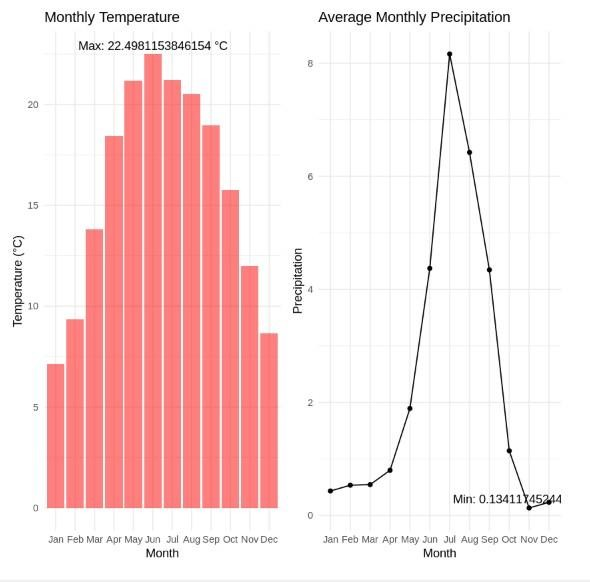
\includegraphics[width=0.5\textwidth]{figures/barchart1.jpg}
\caption{Bar Chart and Line Plot Showing Extreme Events}
\label{fig:dual_extremes}
\end{figure}

\paragraph{How to Interpret These Plots}
\begin{itemize}
  \item The left bar chart clearly marks the month with the highest average temperature.
  \item The right line chart pinpoints the month with the lowest average precipitation.
\end{itemize}

\paragraph{Questions to Explore:}
\begin{itemize}
  \item Does the hottest month align with the driest month?
  \item How do these extremes compare with seasonal expectations in your region?
  \item What implications might this have for agriculture or water resource planning?
\end{itemize}

\subsection*{Seasonal Insights}

\paragraph{Objective:} Identify climate patterns by season to understand how temperature, precipitation, and humidity vary across different times of the year.

\paragraph{Season Classification} To analyze seasonal trends, we categorized each month into one of four standard meteorological seasons:
\begin{itemize}
  \item Spring: March – May
  \item Summer: June – August
  \item Autumn: September – November
  \item Winter: December – February
\end{itemize}

\paragraph{The R code used for classification and aggregation:}

\begin{verbatim}
climate_data$Season <- case_when(
  climate_data$Month_Num %in% c(3,4,5) ~ "Spring",  # Mar-May
  climate_data$Month_Num %in% c(6,7,8) ~ "Summer",  # Jun-Aug
  climate_data$Month_Num %in% c(9,10,11) ~ "Autumn", # Sep-Nov
  climate_data$Month_Num %in% c(12,1,2) ~ "Winter"  # Dec-Feb
)

seasonal_avg <- climate_data %>%
  group_by(Season) %>%
  summarize(
    Avg_Temperature = mean(Temp_2m, na.rm = TRUE),
    Avg_Precipitation = mean(Precip, na.rm = TRUE),
    Avg_Humidity = mean(Humidity_2m, na.rm = TRUE)
  )
\end{verbatim}

\paragraph{Reshaping Data for Visualization}

To visualize all three variables in a single grouped bar chart, the dataset was converted from wide to long format:

\begin{verbatim}
seasonal_avg_long <- seasonal_avg %>%
  gather(key = "Variable", value = "Value", -Season)
\end{verbatim}

\paragraph{Visualization: Seasonal Climate Patterns}

\begin{verbatim}
ggplot(seasonal_avg_long, aes(x = Season, y = Value, fill = Variable)) +
geom_bar(stat = "identity", position = "dodge") +
labs(
title="Seasonal Climate Patterns: Temperature, Precipitation and Humidity",
x = "Season",
y = "Average Value",
fill = "Variable"
) +
theme_minimal()
\end{verbatim}

% Figure here-------------------------
\begin{figure}[h]
\centering
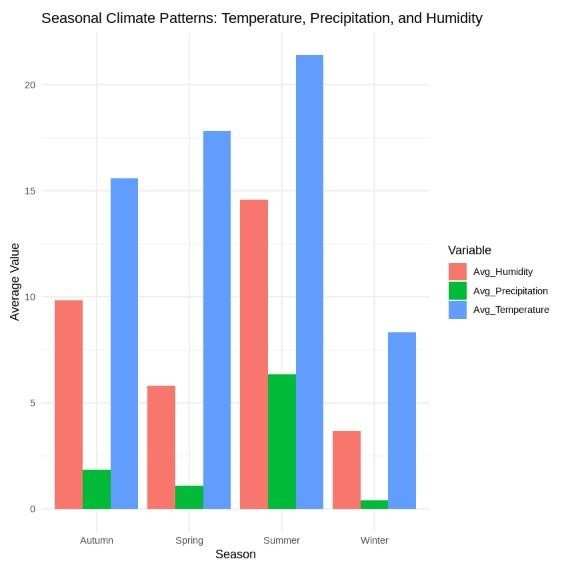
\includegraphics[width=0.5\textwidth]{figures/barchart.jpg}
\caption{Bar Chart Showing Seasonal Climate Pattern}
\end{figure}

\paragraph{Interpretation and Insights} This grouped bar chart shows the average temperature, precipitation, and humidity for each season. It allows for direct comparison across seasons and between variables.

For example, if summer shows high temperature but low humidity and precipitation, it may indicate a dry season.

\paragraph{Interactive Thought:}

Which season experiences the most rainfall? Is that also the most humid? How do these seasonal shifts align with regional agricultural activities or disaster preparedness plans?
\clearpage


 \section{Boxplot: Summarizing Data at a Glance}

Imagine you’re trying to quickly understand how students performed in a test—not just where most scores lie, but also how consistent the scores are and whether any students performed exceptionally well or poorly. A boxplot (also called a box-and-whisker plot) helps us do exactly that.

\subsection*{Key Concepts: Let’s Explore!}

Boxplots are used for numerical data. They show five important numbers that summarize the data:
\begin{itemize}
  \item \textbf{Minimum}: The lowest value in the dataset (excluding extreme outliers).
  \item \textbf{First Quartile (Q1)}: The value below which 25\% of the data falls.
  \item \textbf{Median (Q2)}: The middle value that divides the data into two equal halves.
  \item \textbf{Third Quartile (Q3)}: The value below which 75\% of the data falls.
  \item \textbf{Maximum}: The highest value in the dataset (excluding extreme outliers).
\end{itemize}

\textit{Activity: Can you identify these five values in a small dataset of test scores? Try with: 42, 55, 60, 65, 70, 75, 90}

\paragraph{The Box and the Whiskers}

The box spans from the first quartile (Q1) to the third quartile (Q3). This shows where the middle 50\% of the data lies. It helps us understand the data’s “interquartile range” or IQR.

A line inside the box marks the median.

The whiskers extend from the box to the minimum and maximum values that are not considered outliers.

Any points that lie far outside the whiskers are called outliers and are usually plotted as individual dots or stars.

\subsection*{Why Use Boxplots?}

Boxplots help us see:
\begin{itemize}
  \item \textbf{Skewness}: If the median is not centered in the box or if one whisker is much longer, the data may be skewed.
  \item \textbf{Spread}: A longer box or whiskers mean more variability in the data.
  \item \textbf{Outliers}: Easily spot values that don’t fit the general pattern.
  \item \textbf{Comparison}: Boxplots are great for comparing multiple datasets side by side.
\end{itemize}

\paragraph{Visual Summary: What You Learn at a Glance}

\begin{itemize}
  \item A centered median suggests a symmetric distribution.
  \item A longer upper whisker might suggest a few students scored exceptionally high.
  \item Outliers could represent unusual performances or data entry errors.
\end{itemize}

\subsection*{Example: Let’s Visualize Climate Data}

We can apply a boxplot to climate data to understand temperature variations over the years. For instance, let’s consider the average summer temperature across several years. A boxplot can quickly show:
\begin{itemize}
  \item Whether the temperatures have a consistent range.
  \item If there are any outlier years with unusually hot or cold summers.
  \item Whether the trend has become skewed (perhaps due to climate change).
\end{itemize}

\subsection*{Try it in R!}

\paragraph{Wind Speed Analysis by Altitude}

Wind speed is a crucial component of climate data and can vary significantly with altitude. In this task, we explore how wind speed differs between two common measurement heights: 10 meters and 50 meters above ground level.

Understanding wind speed variability at different altitudes is important for:
\begin{itemize}
  \item Weather forecasting: Accurate wind speed data improves storm tracking and model predictions.
  \item Agricultural planning: Wind affects crop pollination, irrigation patterns, and soil erosion.
  \item Environmental studies: Wind disperses pollutants and influences temperature and humidity distribution.
\end{itemize}

\paragraph{Step 1: Summary Statistics in R}

First, we calculate summary statistics for wind speed at both altitudes using the \texttt{dplyr} package in R:

\begin{verbatim}
summary <- climate_data %>%
  summarise(
    mean_10m = mean(WindSpeed_10m),
    sd_10m = sd(WindSpeed_10m),
    median_10m = median(WindSpeed_10m),
    mean_50m = mean(WindSpeed_50m),
    sd_50m = sd(WindSpeed_50m),
    median_50m = median(WindSpeed_50m)
  )
print(summary)
\end{verbatim}

% Fihgure here -------------------------
\begin{figure}[h]
\centering
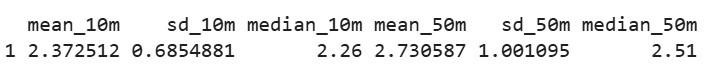
\includegraphics[width=0.6\textwidth]{figures/summ_stats.jpg}
\caption{Summary Statistics}
\end{figure}

This code computes:
\begin{itemize}
  \item Mean: The average wind speed at each height.
  \item Standard deviation (SD): How much the wind speed varies from the mean.
  \item Median: The middle value in the dataset.
\end{itemize}
These measures help us compare central tendency and variability between the two heights.

\paragraph{Step 2: Visual Comparison using Boxplot}

We now visualize the wind speeds using a boxplot:

\begin{verbatim}
boxplot(
  climate_data$WindSpeed_10m, climate_data$MaxWindSpeed_50m,
  names = c("WindSpeed_10m","WindSpeed_50m"),
  main = "Windspeed Comparison",
  xlab = "Windspeed (m/s)",
  col = c("green", "orange")
)
\end{verbatim}

% Figure ------------------------------
\begin{figure}[h]
\centering
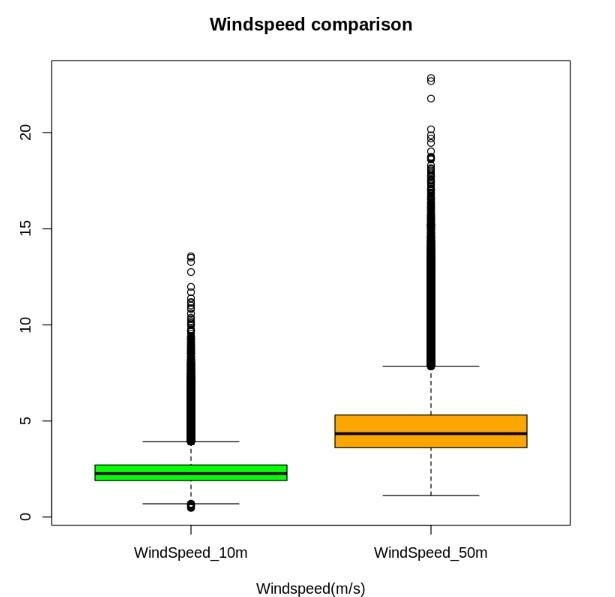
\includegraphics[width=0.5\textwidth]{figures/windspeed.jpg}
\caption{Windspeed Comparison at 10m and 50m}
\end{figure}

This boxplot compares the distribution of wind speed at 10m and 50m heights. Here’s what we observe:
\begin{itemize}
  \item \textbf{Median Line}: Indicates the central value of wind speed for each altitude.
  \item \textbf{Box Size}: Represents the interquartile range (spread of the middle 50\% of values).
  \item \textbf{Whiskers and Outliers}: Show the overall range and any extreme values.
\end{itemize}

\textbf{Discussion} \\

Typically, wind speed increases with altitude due to reduced friction with the Earth’s surface. Therefore, we expect the boxplot for 50m to have:
\begin{itemize}
  \item A higher median compared to 10m.
  \item Possibly greater variability, depending on terrain and weather conditions.
\end{itemize}

\textit{Activity: Can you interpret the difference in medians and spreads between the two boxplots? What might this tell us about wind behavior in the area?}

This analysis demonstrates how simple statistics and visualizations can uncover meaningful patterns in climate data, helping us make more informed decisions in environmental monitoring and planning.

\subsection*{Outliers and Their Significance in Climate Data}

Outliers are data points that significantly deviate from the general pattern of the dataset. In the context of climate analysis, outliers may represent unusual or extreme weather events—such as unexpected temperature spikes, intense rainfall, or strong windstorms. These anomalies are critical for several reasons:
\begin{itemize}
  \item \textbf{Insights into Extreme Events}: Outliers can help identify climatic extremes such as droughts, floods, or heatwaves. Recognizing these events is vital for disaster preparedness and mitigation.
  \item \textbf{Indicators of Data Quality Issues}: Outliers can sometimes indicate sensor errors or mistakes in data recording, highlighting the need for validation.
  \item \textbf{Understanding Climate Trends}: Persistent or frequent outliers might signal larger shifts in climate patterns.
  \item \textbf{Impact on Modeling}: Since outliers can skew statistical models, identifying and treating them appropriately is essential for producing reliable predictions.
\end{itemize}

\textbf{Interquartile Range (IQR) Method for Detecting Outliers}\\

The IQR is a measure of variability, defined as the difference between the third quartile (Q3) and the first quartile (Q1):
\[
\text{IQR} = Q_3 - Q_1
\]

Data points falling outside the following bounds are considered potential outliers:
\[
\text{Lower Bound} = Q_1 - 1.5 \times \text{IQR}, \quad \text{Upper Bound} = Q_3 + 1.5 \times \text{IQR}
\]

\paragraph{R Code: Identifying Outliers Based on Precipitation}

\begin{verbatim}
# Step 1: Calculate IQR and Bounds
Q1 <- quantile(filtered_hilly_data$Precip, 0.25)  # First Quartile (25%)
Q3 <- quantile(filtered_hilly_data$Precip, 0.75)  # Third Quartile (75%)
IQR <- Q3 - Q1  # Interquartile Range
lower_bound <- Q1 - 1.5 * IQR  # Lower bound
upper_bound <- Q3 + 1.5 * IQR  # Upper bound

# Step 2: Identify Outliers
outliers <- filtered_hilly_data
[filtered_hilly_data$Precip <
 lower_bound | filtered_hilly_data$Precip > upper_bound, ]
non_outliers <- filtered_hilly_data
[filtered_hilly_data$Precip >= 
lower_bound & filtered_hilly_data$Precip <= upper_bound, ]
\end{verbatim}

\textbf{Summary Statistics with and without Outliers} \\

Summary statistics are numerical values that describe key features of a dataset. These include measures of central tendency and variability, and are essential for understanding the general behavior of climate data.

\begin{verbatim}
cat("Original Dataset Summary:\n")
summary(filtered_hilly_data$Precip)

cat("\nDataset Without Outliers:\n")
summary(non_outliers$Precip)

cat("\nOutliers Only:\n")
summary(outliers$Precip)
\end{verbatim}

% Figure --------------------------------
\begin{figure}[h]
\centering
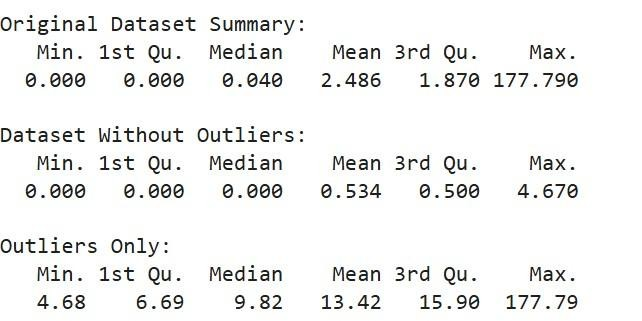
\includegraphics[width=0.6\textwidth]{figures/summary_stats.jpg}
\caption{Summary Statistics}
\end{figure}

\subsection*{Visualizing Outliers with Boxplots} 

\subsubsection*{Boxplot including outliers:}

\begin{verbatim}
ggplot(filtered_hilly_data, aes(x = Month_Label, y = Precip)) +
  geom_boxplot(outliers.colour = "red") +
  theme_minimal() +
  labs(
    title = "Precipitation Variation by Seasons", 
    x = "Month", 
    y = "Precipitation"
    )
\end{verbatim}

\subsubsection*{Boxplot without outliers:}

\begin{verbatim}
ggplot(non_outliers, aes(x = Month_Label, y = Precip)) +
  geom_boxplot() +
  theme_minimal() +
  labs(
    title = "Precipitation Variation by Seasons",
    x = "Month",
    y = "Precipitation"
    )
\end{verbatim}

% Figure here-----------------------------
\begin{figure}[h]
\centering
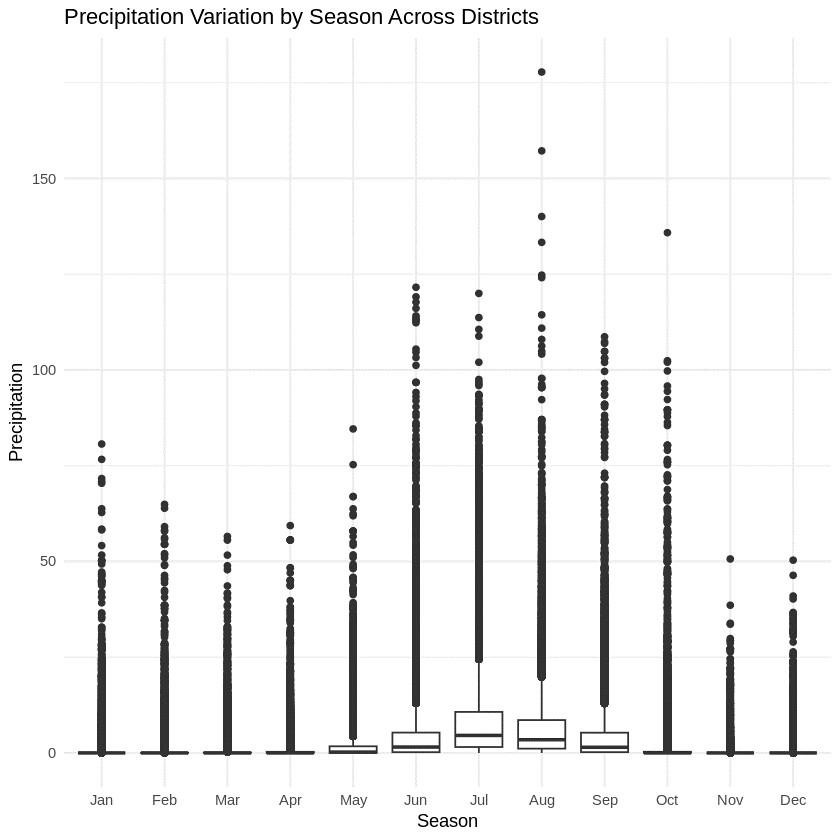
\includegraphics[width=0.5\textwidth]{figures/outliers.jpg}
\caption{Boxplot Showing Outliers}
\end{figure}

% Figure here-----------------------------
\begin{figure}[h]
\centering
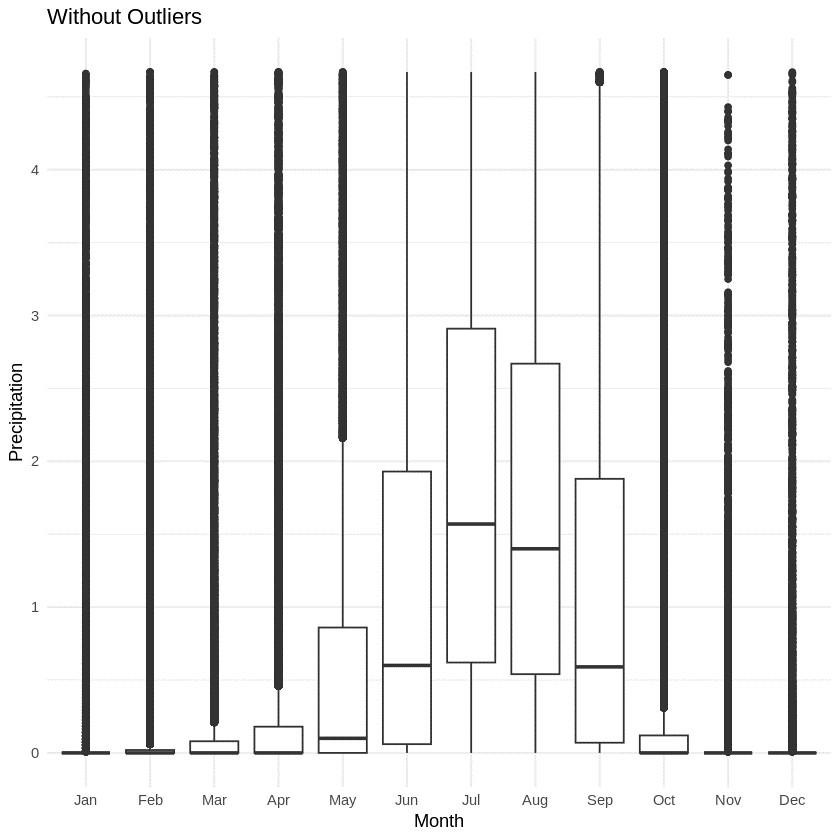
\includegraphics[width=0.5\textwidth]{figures/no_outliers.jpg}
\caption{Boxplot After Removing Outliers}
\end{figure}

\subsection*{Understanding Standard Deviation and Range}

\textbf{1. Standard Deviation}\\

Standard deviation quantifies how much the data deviates from the mean. A higher value indicates that the data points are more spread out, while a lower value suggests they are clustered around the mean.

\paragraph{Formula for Population Standard Deviation:}
\[
\sigma = \sqrt{\frac{1}{N} \sum_{i=1}^N (x_i - \mu)^2}
\]

\paragraph{Formula for Sample Standard Deviation (with Bessel’s correction):}
\[
s = \sqrt{\frac{1}{N-1} \sum_{i=1}^N (x_i - \bar{x})^2}
\]

\paragraph{Interpretation:}
\begin{itemize}
  \item Low standard deviation \(\rightarrow\) Values are close to the mean.
  \item High standard deviation \(\rightarrow\) Values are widely spread.
\end{itemize}

\paragraph{2. Range}

The range is the difference between the maximum and minimum values in the dataset:
\[
\text{Range} = \text{Maximum} - \text{Minimum}
\]

\paragraph{Interpretation:}
\begin{itemize}
  \item Small range \(\rightarrow\) Values are concentrated.
  \item Large range \(\rightarrow\) Values are spread out, possibly due to outliers.
\end{itemize}

\paragraph{R Code: Calculating Standard Deviation and Range}

\begin{verbatim}
cat("\nStandard Deviation with Outliers: ", 
sd(filtered_hilly_data$Precip), "\n")
cat("Standard Deviation without Outliers: ", 
sd(non_outliers$Precip), "\n")

cat("\nRange with Outliers: ", range(filtered_hilly_data$Precip), "\n")
cat("Range without Outliers: ", range(non_outliers$Precip), "\n")
\end{verbatim}

% Figure here--------------------------
\begin{figure}[h]
\centering
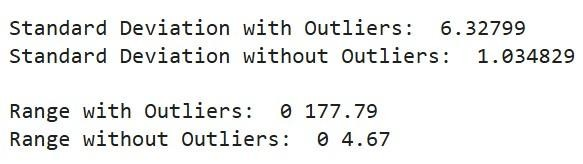
\includegraphics[width=0.6\textwidth]{figures/sd_range.jpg}
\caption{Standard Deviation and Range Calculation}
\end{figure}

\paragraph{Results Interpretation}

\begin{itemize}
  \item \textbf{Standard Deviation}:
  \begin{itemize}
    \item With outliers: 6.33
    \item Without outliers: 1.03
  \end{itemize}
  Outliers significantly increase the standard deviation, exaggerating the variability in precipitation data.
  
  \item \textbf{Range}:
  \begin{itemize}
    \item With outliers: 0 to 177.79
    \item Without outliers: 0 to 4.67
  \end{itemize}
  The range is greatly inflated by extreme values, demonstrating how outliers can distort the data distribution.
\end{itemize}

\paragraph{Points to Note}

\begin{itemize}
  \item Outliers make the data appear more variable than it actually is.
  \item Removing outliers can help clarify typical climate patterns.
  \item If the goal is to understand extreme events (like floods or heavy rain), outliers should be analyzed, not discarded.
\end{itemize}
However, if you’re trying to understand the more typical patterns in the data, removing the outliers might give you a clearer picture.

\clearpage

 \section{Geographical Plot: Visualizing Spatial Data}

In climate data analysis, geographical visualization plays a crucial role in understanding spatial variations across regions. Spatial data—such as district boundaries—can be combined with climate variables like temperature and precipitation to generate meaningful visual maps. These maps help reveal regional patterns that might not be obvious through tables or charts.

By visually overlaying climate information on geographic regions, researchers can detect hotspots, identify vulnerable areas, and observe spatial trends over time. Such visual tools enhance decision-making for climate adaptation strategies, regional planning, and policy development. Moreover, they improve the communication of complex climate data to stakeholders, including policymakers and the general public.

In this section, we demonstrate how to visualize spatial climate data using the \texttt{ggplot2} and \texttt{sf} packages in R. We utilize a shapefile representing the administrative boundaries of Nepal’s districts and merge it with district-level climate summaries to create intuitive thematic maps.

The shapefile provides the spatial structure (geometry) of the districts, while the associated dataset includes numerical climate values, such as average temperature and average precipitation for each district. Once merged, this combined data is plotted on a map, where color gradients represent climate intensity.

These visualizations offer a powerful way to interpret and communicate geographic patterns in climate data. They are especially useful in climate vulnerability assessment, disaster preparedness, and resource planning.

\subsection*{Shapefile Source}

The shapefile used for the geographical plots was obtained from Open Data Nepal. You can download it from the following link:

\href{https://opendatanepal.com/dataset/new-political-and-administrative-boundaries-shapefile-of-nepal}{Download shapefile of Nepal from here}

A typical shapefile set consists of multiple files including \texttt{.shp}, \texttt{.shx}, \texttt{.dbf}, \texttt{.prj}, \texttt{.cpg}, and \texttt{.qpj}.  These files work together to store not only the boundary shapes but also the related attributes and coordinate information required for accurate mapping.

In this project, the shapefile was essential for creating district-wise maps to visualize climate variables like temperature and precipitation. Before using the shapefile in R, it was loaded using spatial packages such as sf , and then joined with climate datasets based on matching district names. This allowed for layered visualizations where climate trends could be examined within their real-world geographic context


\subsection*{Required R Packages}

To run the spatial data visualizations and maps in this chapter, the following R packages must be installed and loaded:
\begin{itemize}
  \item ggmap – for base map overlays and geospatial mapping
  \item sf – for handling simple feature (spatial) data 
  \item rnaturalearth and rnaturalearthdata – for accessing natural earth map data

Use the following R commands to install and load the packages:

\end{itemize}
\begin{verbatim}
install.packages("ggmap")
install.packages("sf")
library(sf)
install.packages(c("rnaturalearth", "rnaturalearthdata"))
library(rnaturalearth)
library(rnaturalearthdata)
\end{verbatim}

\subsection*{Preparing the Shapefile for Merging}

After loading the shapefile containing Nepal’s district boundaries, the next step is to examine its structure and identify the column containing district names. This is necessary for merging the spatial data with the corresponding climate data.

\begin{verbatim}
# Load the new Nepal district shapefile
nepal_districts <- st_read("/content/shapes")

# Check column names in each dataset
colnames(nepal_districts)
\end{verbatim}

% Figure here ----------------------------
\begin{figure}[h]
\centering

\includegraphics[width=1.02\textwidth]{figures/column_names.jpg}
\caption{Column names in shapefile}
\label{fig:shapefile_columns}
\end{figure}

Upon inspecting the column names, identify the one that corresponds to district names. Here, the relevant column is \texttt{dist\_name}, which should be renamed to match the corresponding column in the climate dataset (\texttt{District}):

\begin{verbatim}
# Rename the district name column for consistency
nepal_districts <- nepal_districts %>% rename(District = dist_name)
\end{verbatim}

This ensures consistency between the spatial dataset and the climate dataset, allowing them to be merged correctly based on the \texttt{District} column.

\subsection*{Reconciling District Names between Shapefile and Climate Dataset}

Before we can merge the shapefile data with our climate dataset, we need to make sure that the names of the districts match across both sources. This is important because even small differences in spelling or naming style can cause the merge to fail or produce incorrect results.

To check for mismatches, we first view the unique district names in each dataset:

\begin{verbatim}
# View district names
unique(nepal_districts$District)
unique(df_climate$District)

\end{verbatim}


\subsection*{Merging Spatial and Climate Data}

We calculate the average temperature and precipitation for each district from the climate dataset:

\begin{verbatim}
plot_by_district <- df_climate %>%
  group_by(District) %>%
  summarise(
    avg_temp = mean(Temp_2m, na.rm = TRUE),
    avg_precip = mean(Precip, na.rm = TRUE),
    Latitude = first(Latitude),
    Longitude = first(Longitude)
  )
\end{verbatim}

These outputs show the mismatches: names from the shapefile that don’t exist in the climate data, and vice versa.

After identifying the mismatched names, we create a mapping to fix them:

\begin{verbatim}

# Verify unmatched districts
setdiff(unique(nepal_districts$District), plot_by_district$District)

setdiff(plot_by_district$District, unique(nepal_districts$District))

#Output
"Bajhang", "Bajura", "Kalikot", "Achham", "Jajarkot", "Dolakha", "Tanahu",
"Chitwan", "Ramechhap", "Kavrepalanchok", "Bhojpur", "Khotang", "Panchthar", 
"Sindhupalchok", "Rolpa", "Pyuthan", "Kapilbastu", "Parsa", "Tehrathum",
"Rautahat", "Siraha"

"Bajang", "Chitawan", "Dolkha", "Kabhre", "Panchther", "Routahat", 
"Tanahun", "Terhathum"
\end{verbatim}

After identifying the mismatched names, we create a mapping to fix them:
\begin{verbatim}
  # Create mapping for mismatched district names
district_map <- c(
  "Bajhang" = "Bajang",
  "Chitwan" = "Chitawan",
  "Dolakha" = "Dolkha",
  "Kavrepalanchok" = "Kabhre",
  "Panchthar" = "Panchther",
  "Rautahat" = "Routahat",
  "Tanahu" = "Tanahun",
  "Tehrathum" = "Terhathum"
)

# Apply the mapping to the District column
nepal_districts <- nepal_districts %>%
  mutate(District = recode(District, !!!district_map))
\end{verbatim}

This transformation ensures that the \texttt{District} column in the shapefile matches the corresponding column in the climate data, allowing for a successful merge. The use of the \texttt{!!} operator in \texttt{recode()} allows for unpacking the named vector.

Finally, we merge the cleaned shapefile data with the summarized climate data:
\begin{verbatim}
nepal_map_data <- left_join(nepal_districts, plot_by_district, 
by = "District")
\end{verbatim}

This completes the data preparation step, combining spatial and climate information for each district. Now, we can move on to visualizing the climate data on the map of Nepal.

\subsection*{Temperature Map of Nepal}

Spatial visualization of climate data enables an intuitive understanding of regional variations. A temperature map highlights how average temperatures vary across districts, helping identify hot and cold zones. Such visual tools are essential in studying local climate impacts, regional heat stress, and potential vulnerabilities in agriculture or health sectors.

The following R code loads a shapefile of Nepal’s districts, merges it with temperature data, and visualizes average temperatures using \texttt{ggplot2}:

\begin{verbatim}
ggplot(data = nepal_map_data) +
  geom_sf(aes(fill = avg_temp), color = "black") +  # Fill districts
  geom_text(data = plot_by_district, aes(x = Longitude, 
  y = Latitude, label = District),
            size = 1.5, vjust = -0.5, color = "black") +
  scale_fill_gradient(low = "yellow", high = "red") +  # Color scale
  labs(title = "Temperature Map of Nepal", fill = "Temperature") +
  theme_minimal()
\end{verbatim}

% Figure here -------------------------
\begin{figure}[h]
\centering
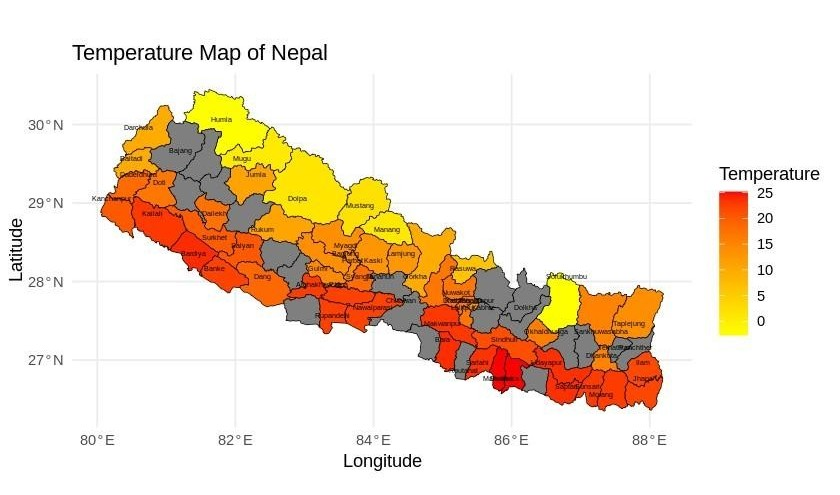
\includegraphics[width=0.6\textwidth]{figures/geo_temp.jpg}
\caption{Geoplot showing temperature distribution in Nepal}
\label{fig:temp_map_nepal}
\end{figure}

\subsection*{Precipitation Map of Nepal}

Precipitation mapping reveals the spatial distribution of rainfall, which is crucial for water resource management, agriculture, and flood risk assessment. By visualizing average precipitation at the district level, we can identify regions with excessive or insufficient rainfall, guiding decisions in irrigation planning and disaster preparedness.

\begin{verbatim}
ggplot(data = nepal_map_data) +
  geom_sf(aes(fill = avg_precip), color = "black") +  
  geom_text(data = plot_by_district, aes(x = Longitude, y = Latitude, 
  label = District),
            size = 1.5, vjust = -0.5, color = "black") +
  scale_fill_gradient(low = "skyblue", high = "blue") +  
  labs(title = "Precipitation Map of Nepal", fill = "Precipitation") +
  theme_minimal()
\end{verbatim}

% figure here ---------------------------
\begin{figure}[h]
\centering
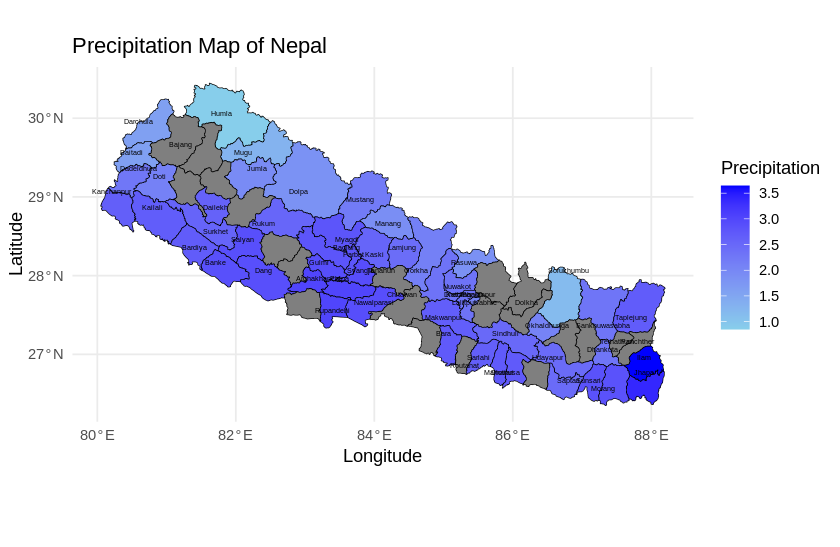
\includegraphics[width=0.6\textwidth]{figures/geo_precip.png}
\caption{Geoplot showing precipitation distribution in Nepal}
\label{fig:precip_map_nepal}
\end{figure}

 \section{Time Series Plot: Visualizing Trends Over Time}

Time series plots are essential tools in climate data analysis, allowing researchers to observe and interpret variations in a variable over time. A time series consists of data points collected or recorded at successive time intervals typically days, months, or years.

In climate science, variables such as temperature, precipitation, humidity, and pressure are often monitored over long periods. Plotting these values against time helps to identify seasonal patterns, trends, anomalies, and long-term climate changes.

Time series plots make it easier to detect cycles (like monsoon seasons), abrupt changes (such as droughts or floods), and overall trends (such as rising temperatures due to climate change). They are also useful for comparing trends across multiple locations or climate indicators.

In this section, we use R to generate time series plots using the \texttt{ggplot2} package. These plots provide a visual summary of climate variables, offering intuitive insights into their temporal behavior.

\subsection*{Precipitation and Temperature Over Time}

The following R code generates a time series plot comparing precipitation and temperature over time, using different colors for each variable.

\begin{verbatim}
ggplot(df_climate, aes(x = Date)) +
  geom_line(aes(y = Precip, color = 'Precipitation'), linewidth = 1) +
  geom_line(aes(y = Temp_2m, color = 'Temperature'), linewidth = 1) +
  labs(title = 'Precipitation and Temperature Over Time',
       x = 'Date',
       y = 'Values') +
  scale_color_manual(name = 'Legend', 
    values = c('Precipitation' = 'blue', 'Temperature' = 'orange')) +
  theme(legend.position = 'top')  # Adjust legend position as needed
\end{verbatim}

% Figure here---------------------------
\begin{figure}[h]
\centering
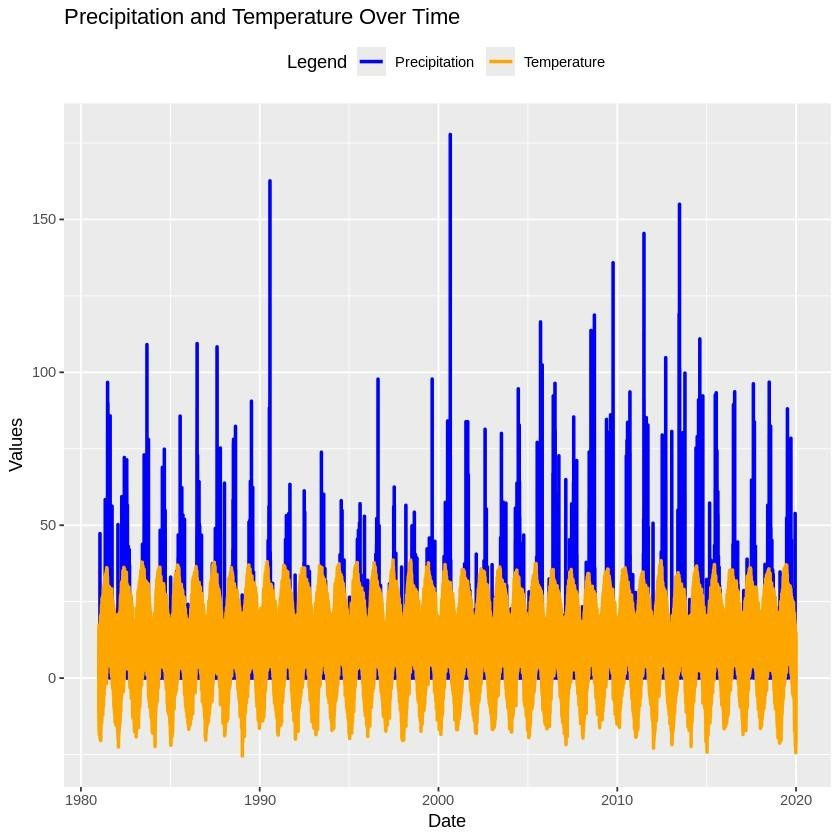
\includegraphics[width=0.5\textwidth]{figures/temp_precipt.jpg}
\caption{Temperature and Precipitation Over Time}
\end{figure}

\subsection*{Yearly Trend Analysis of Temperature}

The R code below calculates average temperature, precipitation, and humidity per year and plots the temperature trend over time with a smoothed line.

\begin{verbatim}
df_yearly <- df_climate %>%
  group_by(Year = format(Date, "%Y")) %>%
  summarise(
    AvgTemp = mean(Temp_2m, na.rm = TRUE),
    AvgPrecip = mean(Precip, na.rm = TRUE),
    AvgHumidity = mean(Humidity_2m, na.rm = TRUE)
  )

# Plot the trend over years
ggplot(df_yearly, aes(x = as.numeric(Year), y = AvgTemp)) +
geom_line(color = "blue", size = 1) + 
geom_point(color = "red") +  
geom_smooth(method = "loess", color = "darkgreen", 
linetype = "dashed", size = 1, se = FALSE) +# Smoothed trend line
labs(title = "Trend Analysis of Temperature Over Years",
       x = "Year",
       y = "Average Temperature (°C)") +
scale_x_continuous(
breaks = seq(min(df_yearly$Year),
max(df_yearly$Year), by = 2)) +  # Set interval
theme_minimal() +
theme(axis.text.x = element_text(angle = 45, hjust = 1))
\end{verbatim}

% Figure here-----------------------------
\begin{figure}[h]
\centering
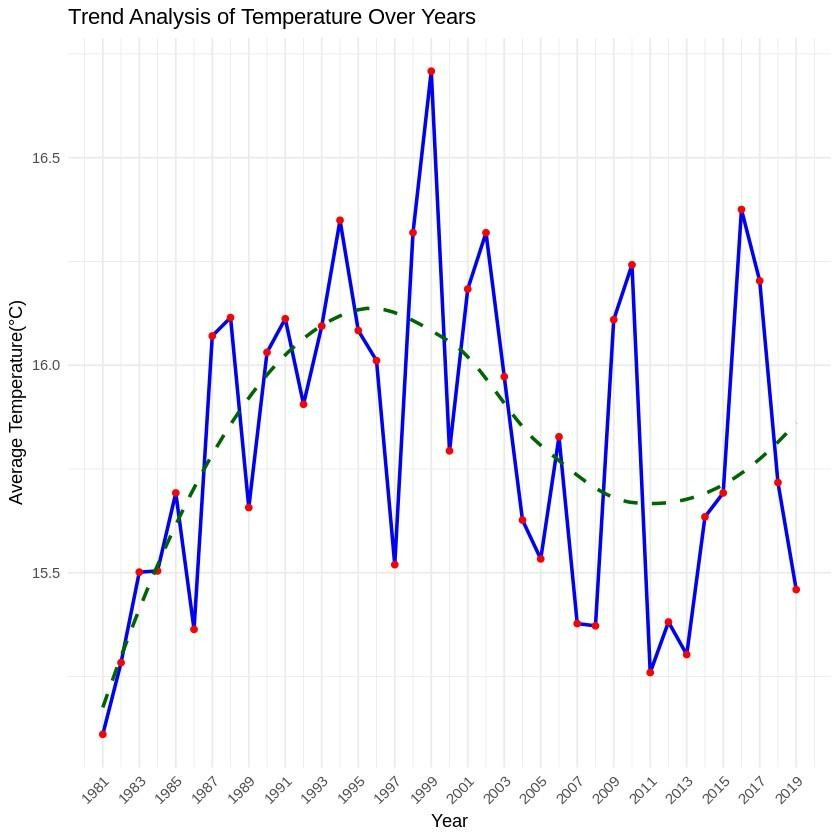
\includegraphics[width=0.5\textwidth]{figures/temp_trend.jpg}
\caption{Temperature Trend Over Years}
\end{figure}

\subsection*{Yearly Trend Analysis of Precipitation}

This R script shows how average precipitation changes over time using a line and smoothed trend plot.

\begin{verbatim}
# Plot the trend over years
ggplot(df_yearly, aes(x = as.numeric(Year),
y = AvgPrecip)) +
  geom_line(color = "blue", size = 1) +    
  geom_point(color = "red") +           
  geom_smooth(method = "loess", color = "darkgreen", 
              linetype = "dashed", size = 1, se = FALSE) +  
  labs(title = "Trend Analysis of Precipitation Over Years",
       x = "Year",
       y = "Average Precipitation (mm/day)") +
  scale_x_continuous(
  breaks = seq(min(df_yearly$Year),
  max(df_yearly$Year), 
  by = 2)) +  # Set interval
  theme_minimal() +
  theme(axis.text.x = element_text(angle = 45, hjust = 1))
\end{verbatim}

% figure here--------------------------
\begin{figure}[h]
\centering
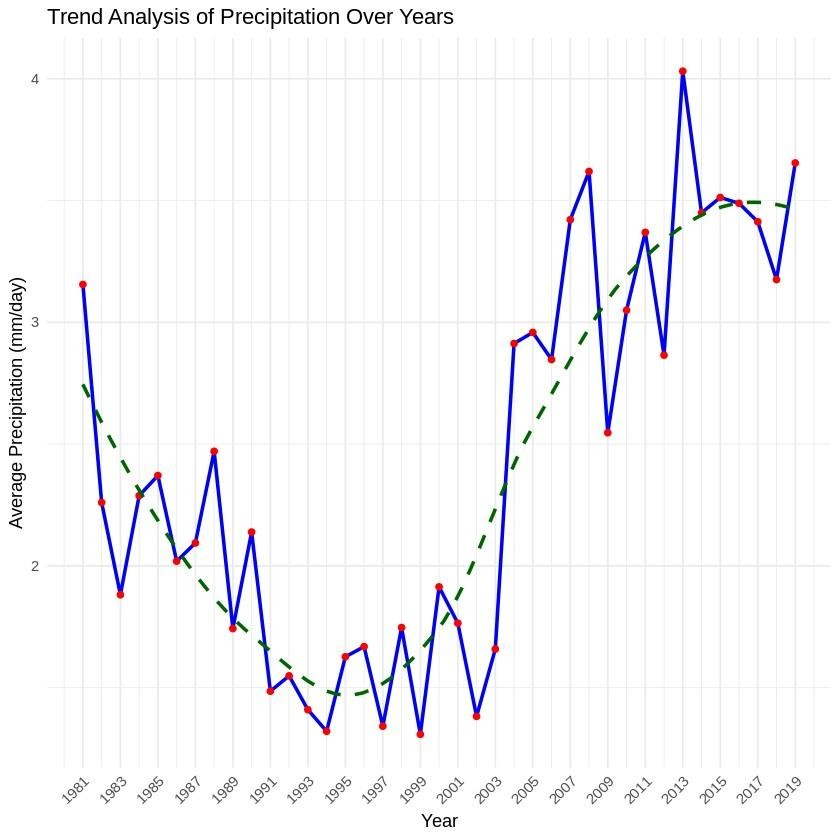
\includegraphics[width=0.5\textwidth]{figures/precip_trend.jpg}
\caption{Precipitation Trend Over Years}
\end{figure}

\chapter{Data Slicing}

\section*{What is Data Slicing?}

Data slicing is the process of selecting specific parts of a dataset, such as certain rows, columns, or time intervals, for focused analysis. Think of a data set as a large spreadsheet with rows (observations) and columns (variables). Data slicing allows us to extract only the portion we need at the moment. It is a crucial skill in data analysis because it helps us to understand and work with complex data more efficiently.

\section*{Why is Data Slicing Important?}

Data slicing is important for several reasons:
\begin{itemize}
    \item \textbf{Focus on relevant data:} We rarely need the entire dataset at once. Slicing helps us extract just the part we want to study.
    \item \textbf{Improve performance:} Working with smaller subsets reduces memory usage and increases speed, especially for large datasets.
    \item \textbf{Enable deeper insights:} Slicing lets us compare specific groups, such as cities, months, or weather types, within the data set.
    \item \textbf{Prepare for visualization:} Often we only want to visualize a specific variable or a time frame, not the whole dataset.
    \item \textbf{Aid in cleaning and validation:} We can inspect subsets for missing or abnormal values more easily.
\end{itemize}

\section*{Common Types of Slicing}

\begin{itemize}
    \item \textbf{Row Slicing:} Selecting specific observations (e.g., all records for March 2021).
    \item \textbf{Column Slicing:} Selecting specific variables (e.g., only Date and Temperature).
    \item \textbf{Conditional Slicing:} Filtering rows based on conditions (e.g., Temperature > 35 °C).
    \item \textbf{Time-based Slicing:} Extracting data for certain dates or periods.
    \item \textbf{Group-based Slicing:} Filtering data by category (e.g., one district or season).
\end{itemize}

\section*{Examples in R}

\subsection*{Basic Row and Column Slicing}
\begin{verbatim}
# First 10 rows and first 3 columns 
df_climate[1:10, 1:3]
\end{verbatim}

\subsection*{Slicing with Conditions}
\begin{verbatim}
# Days with rainfall greater than 10 mm
df_climate[df_climate$Rainfall > 10, ]
\end{verbatim}

\subsection*{Using \texttt{dplyr} for Readability}
\begin{verbatim}
library(dplyr)
# Days in July with temperature above 32 °C 
df_climate %>% filter(month(Date) == 7, Temperature > 32)
\end{verbatim}

\subsection*{Slicing Time Ranges Using \texttt{tsibble}}
\begin{verbatim}
library(tsibble)
# Data between 2020-06-01 and 2020-08-31 
df_climate %>%
  filter(Date >= as.Date("2020-06-01") & Date <= as.Date("2020-08-31"))
\end{verbatim}

\subsection*{Group-based Slicing}
\begin{verbatim}
# Data for only "Kathmandu" district
df_climate %>%
  filter(District == "Kathmandu")
\end{verbatim}

\section*{Useful Libraries for Data Slicing in R}

\begin{itemize}
    \item \textbf{dplyr} : Offers functions like \texttt{filter()}, \texttt{select()}, \texttt{slice()}, and \texttt{arrange()} for easy row/column selection.
    \item \textbf{tsibble} : Ideal for time series slicing. Lets you work with indexed time data.
    \item \textbf{lubridate} : Helps extract parts of a date (e.g., year, month, weekday) for conditional filtering.
    \item \textbf{data.table} : Very fast slicing, great for large datasets. Syntax is concise and powerful.
\end{itemize}

\section*{Best Practices for Data Slicing}

\begin{itemize}
    \item Use descriptive column names for easier selection.
    \item Always check the structure of your data using \texttt{str()} or \texttt{glimpse()} before slicing.
    \item When slicing by date, ensure the column is in Date format using \texttt{as.Date()}.
    \item Chain multiple operations with \texttt{dplyr} to make slicing more readable.
\end{itemize}

\section{Hilly Region Data Analysis}

The following code filters climate data for selected districts in Nepal’s hilly region and prepares it for a temperature distribution map.

\subsection*{Filtering Districts and Calculating Averages}

\begin{verbatim}
# Create a vector of districts to filter
districts_to_filter <- c("Arghakhanchi","Baglung",
"Baitadi", "Bhaktapur", "Chitwan","Dadeldhura",
"Dailekh", "Dhading", "Dhankuta",  "Dolpa", "Gorkha", 
"Gulmi", "Ilam", "Jumla","Kabhre", "Kaski", 
"Kathmandu", "Lalitpur", "Lamjung", 
"Makwanpur", "Myagdi", 
"Nuwakot", "Okhaldhunga", "Palpa", "Parbat", 
"Rukum", "Salyan", "Sindhuli", "Surkhet",
"Syangja")

# Filter the dataset to only include these districts
filtered_hilly_data <- subset(df_climate, District %in% districts_to_filter)

dim(filtered_hilly_data)
# 413076 25  # example output rows and columns
\end{verbatim}

\subsection*{Geoplot for Temperature Distribution in Hilly Region}

\begin{verbatim}
# Calculate average temperature per district
plot_hilly <- filtered_hilly_data %>%
  group_by(District) %>%
  summarise(
    avg_temp = mean(Temp_2m, na.rm = TRUE),
    avg_precip = mean(Precip, na.rm = TRUE),
    Latitude = first(Latitude),
    Longitude = first(Longitude)
  )

# Merge temperature data with spatial data
nepal_temp_hilly <- left_join(nepal_districts, plot_hilly, by = "District")
\end{verbatim}

% Figure here----------------------------
\begin{figure}[h]
\centering
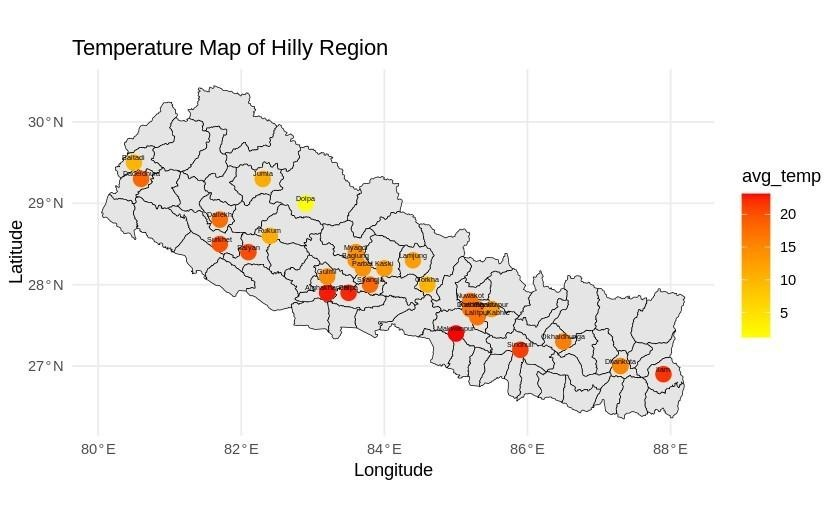
\includegraphics[width=0.6\textwidth]{figures/hilly_map.jpg}
\caption{Temperature Distribution in Nepal using Geoplot
}
\end{figure}

\subsection*{Temperature vs Humidity in the Hilly Region}

The following scatter plot visualizes the relationship between temperature and humidity across districts in the hilly region, colored by season:

\begin{verbatim}
ggplot(filtered_hilly_data, aes(x = Temp_2m, y = Humidity_2m)) +
  geom_point(aes(color = Season), alpha = 0.6) +
  theme_minimal() +
  labs(title = "Temperature vs Humidity in the Hilly Region",
       x = "Temperature (°C)",
       y = "Humidity (%)")
\end{verbatim}

% figure here----------------------------
\begin{figure}[h]
    \centering
    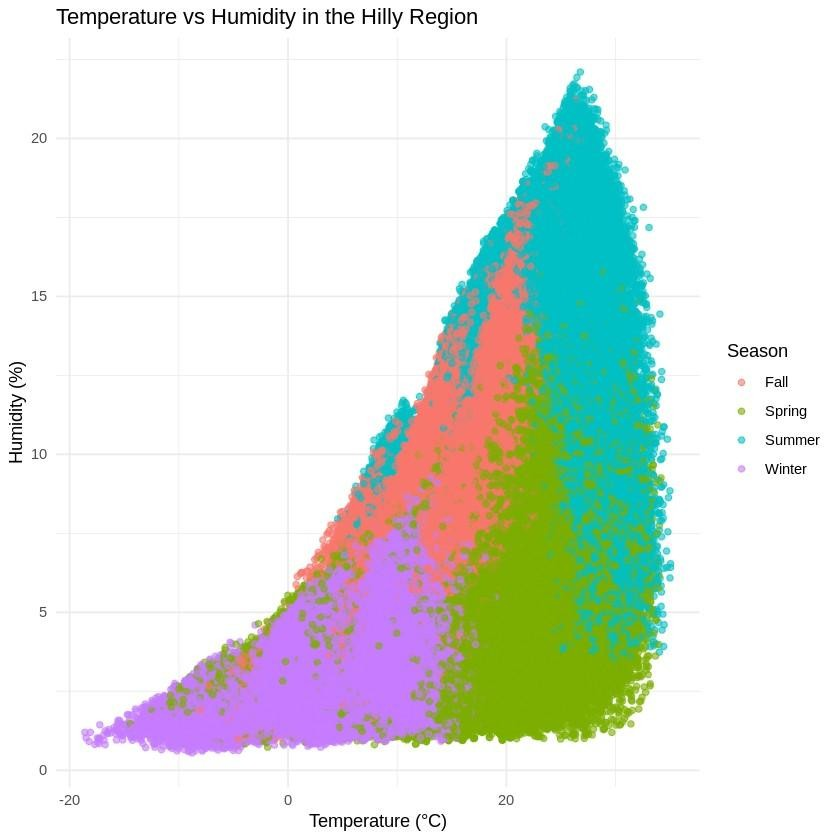
\includegraphics[width=0.5\textwidth]{figures/scatter_hilly.jpg}
    \caption{Scatterplot showing temperature vs humidity according to season}
\end{figure}

\subsubsection*{Insights from Temperature vs Humidity Plot}

\begin{itemize}
    \item A clear positive correlation is observed: higher temperatures generally correspond to higher humidity levels.
    \item Summer shows the highest humidity values, especially above 20\% humidity at moderate to high temperatures.
    \item Winter has the lowest humidity values, often below 10\% even at lower temperatures.
    \item Fall and Spring seasons occupy the middle humidity range, suggesting transitional moisture conditions.
    \item Humidity increases non-linearly with temperature, indicating stronger moisture-holding capacity at warmer temperatures.
    \item A dense clustering of points in summer highlights more consistent humid conditions during that season.
    \item Wider spread of points in winter and spring indicates greater variability in humidity for similar temperature levels.
\end{itemize}

\subsection*{Average Precipitation by District}

\begin{verbatim}
avg_precip_by_district <- filtered_hilly_data %>%
  group_by(District) %>%
  summarise(avg_precip = mean(Precip, na.rm = TRUE))

ggplot(avg_precip_by_district, aes(x = reorder(District, -avg_precip),
 y = avg_precip)) +
  geom_bar(stat = "identity", fill = "skyblue") +
  theme_minimal() +
  labs(title = "Average Precipitation by District",
       x = "District", y = "Average Precipitation") +
  theme(axis.text.x = element_text(angle = 90, hjust = 1))
\end{verbatim}

% Figure here----------------------------
\begin{figure}[h]
    \centering
    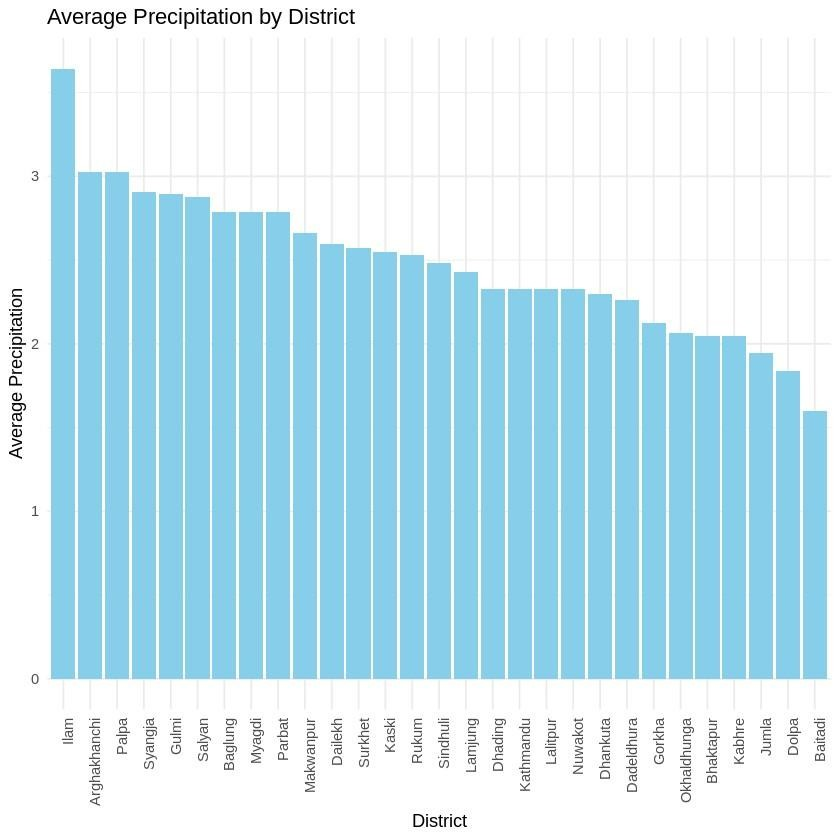
\includegraphics[width=0.5\textwidth]{figures/bar_hilly.jpg}
    \caption{Bar Chart of Average Precipitation in Hilly Region Districts}
\end{figure}

\subsection*{Boxplot of Seasonal Precipitation in Hilly Districts}

\begin{verbatim}
ggplot(filtered_hilly_data, aes(x = Season, y = Precip, fill = Season)) +
  geom_boxplot() +
  labs(title = "Seasonal Precipitation in Hilly Districts",
       x = "Season", y = "Precipitation (mm)") +
  theme_minimal()
\end{verbatim}

% Figure here-----------------------------
\begin{figure}[h]
    \centering
    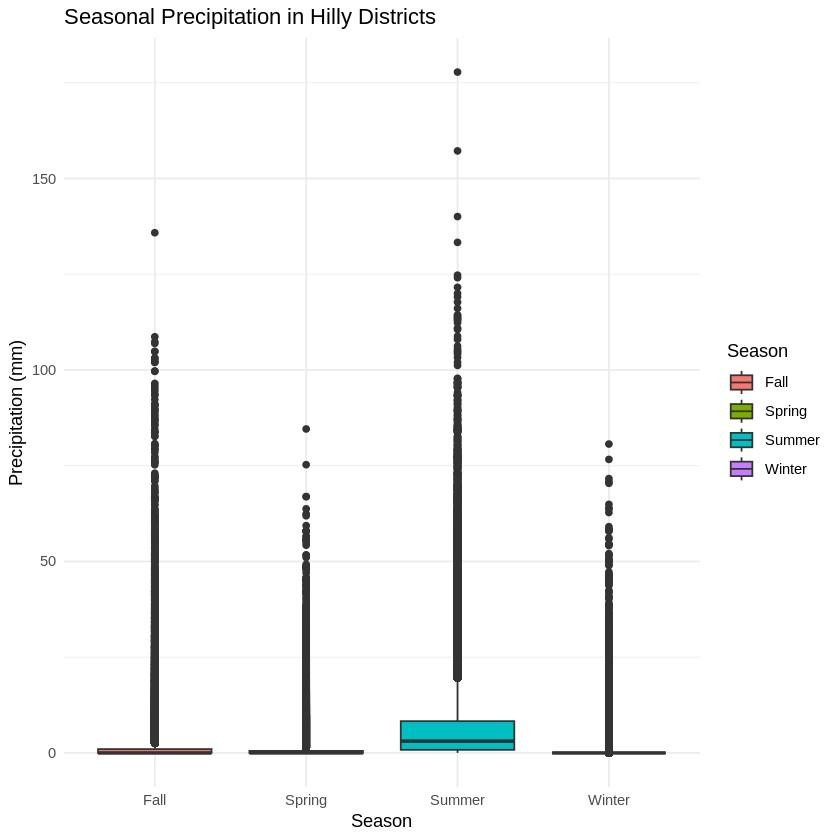
\includegraphics[width=0.5\textwidth]{figures/box_hilly.jpg}
    \caption{Seasonal Precipitation Distribution in Hilly Districts}
\end{figure}

\subsubsection*{Insights from Seasonal Precipitation Plot}

\begin{itemize}
    \item Summer records the highest median and variability in precipitation, indicating it as the peak rainy season.
    \item Spring, Fall, and Winter show comparatively lower median precipitation, clustered near zero.
    \item Despite low medians, all seasons exhibit outliers with precipitation events exceeding 100 mm.
    \item The box for Summer is significantly taller, suggesting a broader interquartile range and more frequent moderate to heavy rainfalls.
    \item Fall and Winter have tight boxes with few extreme outliers, indicating rare but intense rain events.
    \item Spring shows almost no visible box, suggesting highly concentrated low precipitation with sporadic extremes.
    \item Overall, precipitation in hilly districts is highly seasonal, with summer dominating rainfall contributions.
\end{itemize}

\subsection*{Density Plot of Relative Humidity Across Hilly Districts}

\begin{verbatim}
ggplot(filtered_hilly_data, aes(x = RH_2m, fill = District)) +
  geom_density(alpha = 0.4) +
  labs(title = "Humidity Distribution Across Hilly Districts",
       x = "Relative Humidity (%)", y = "Density") +
  theme_minimal()
\end{verbatim}

\begin{figure}[h]
    \centering
    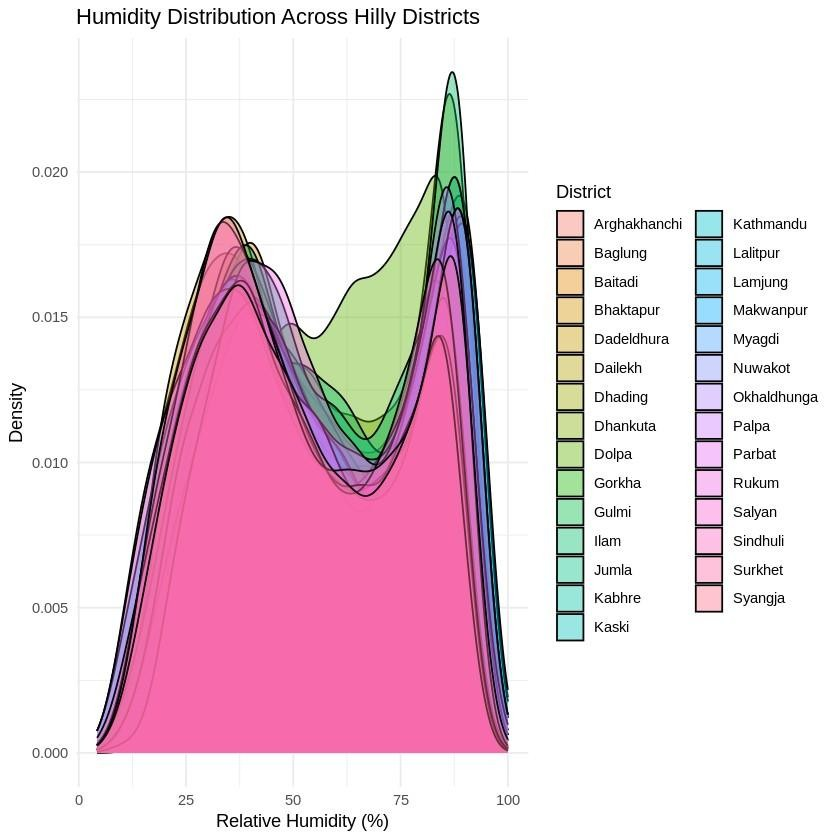
\includegraphics[width=0.5\textwidth]{figures/humid_hilly.jpg}
    \caption{Humidity Distribution Across Hilly Districts}
\end{figure}

\subsubsection*{Insights from Humidity Distribution}

\begin{itemize}
    \item The distribution is bimodal, indicating distinct dry and wet seasonal patterns.
    \item High relative humidity levels (75–90\%) are common across many districts.
    \item Districts like Rukum show broader density curves, suggesting higher variability in humidity.
    \item Districts such as Kathmandu and Dhankuta have sharper peaks, indicating more stable humidity conditions.
    \item Overlapping curves among districts point to similar climatic conditions in the hilly region.
    \item Tails extending towards 0\% and 100\% imply the occurrence of rare extreme humidity events.
    \item These patterns help identify humidity-prone areas useful for agricultural and climatic planning.
\end{itemize}

\subsection*{Extreme Precipitation Analysis in Hilly Regions}

Understanding extreme rainfall events is crucial for disaster preparedness, especially in hilly terrains where intense precipitation can trigger flash floods and landslides. This section presents an analysis of high-impact rainfall events in such regions based on the 95th percentile threshold.

\subsubsection*{Monthly Precipitation Trends}

We begin by computing average monthly precipitation for each year to examine seasonal variation.

\begin{verbatim}
monthly_precip_hilly <- filtered_hilly_data %>%
  group_by(Month_Number, Year = as.numeric(format(Date, "%Y"))) %>%
  summarize(Avg_Precip = mean(Precip, na.rm = TRUE))
\end{verbatim}

\subsubsection*{Defining Extreme Rainfall Events}

To isolate extreme rainfall events, we compute the 95th percentile of all precipitation values. Events exceeding this threshold are classified as extreme.

\begin{verbatim}
# Calculate the 95th percentile of Precipitation
extreme_threshold <- quantile(filtered_hilly_data$Precip, 0.95, na.rm = TRUE)

# Filter the extreme events
extreme_events_hilly <- filtered_hilly_data %>%
filter(Precip > extreme_threshold)

print(extreme_threshold)

95%
13.51
\end{verbatim}

\subsubsection*{Yearly Trend of Extreme Events}

We extract the year from each event and calculate the yearly frequency of extremes to visualize how often such events occur over time.

\begin{verbatim}
# Extract year and count extreme events per year
extreme_events_hilly$Year <- format(extreme_events_hilly$Date, "%Y")
yearly_extreme <- extreme_events_hilly %>%
group_by(Year) %>%
  summarize(Count = n())

# Plot yearly frequency
ggplot(yearly_extreme, aes(x = as.numeric(Year), y = Count)) +
geom_line() +
geom_point() +
labs(
  title = "Yearly Frequency of Extreme Precipitation Events",
  x = "Year",
  y = "Number of Extreme Events")
\end{verbatim}

% Figure here-----------------------------
\begin{figure}[h]
    \centering
    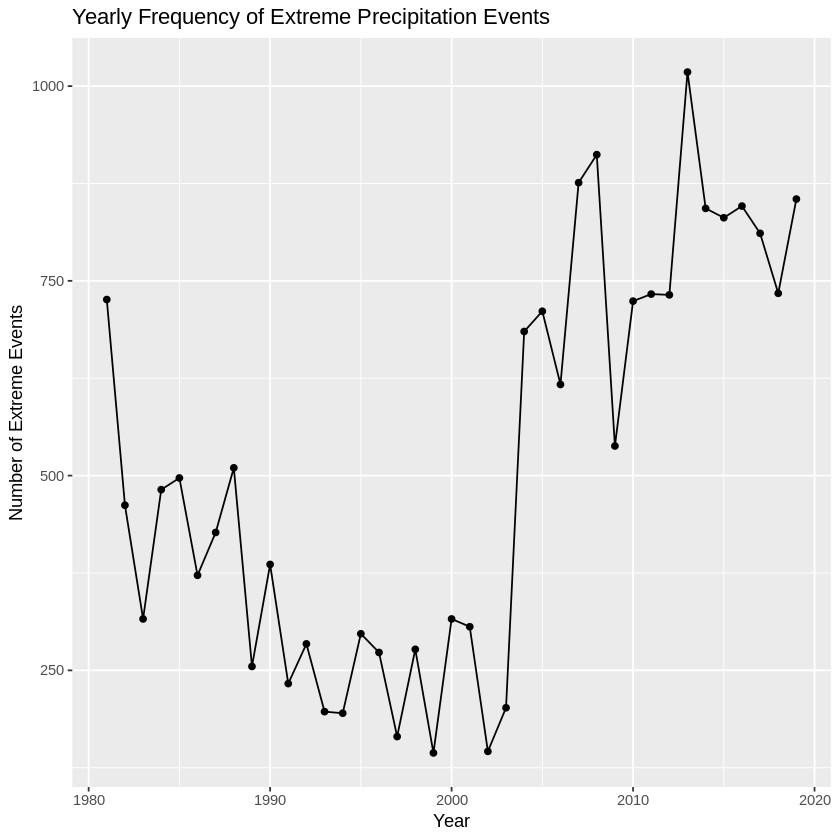
\includegraphics[width=0.5\textwidth]{figures/trend_hilly.jpg}
    \caption{Yearly Frequency of Extreme Precipitation Events}
\end{figure}

\subsubsection*{Yearly Trends}

\begin{itemize}
    \item Low and fluctuating frequency of extreme events from 1980 to early 2000s.
    \item Sharp increase in events post-2003, with a peak around 2013.
    \item Suggests rising climate variability and increased flood risk in recent decades.
\end{itemize}

\subsubsection*{Monthly Distribution of Extreme Events}

To identify seasonal flood risk, we count the number of extreme events in each month and visualize the distribution.

\begin{verbatim}
# Count extreme events per month
monthly_extremes <- extreme_events_hilly %>%
group_by(Month_Label) %>%
  summarize(Count = n())

# Plot the counts
ggplot(monthly_extremes, aes(x = Month_Label, y = Count)) +
geom_bar(stat = "identity", fill = "red") +
labs(
  title = "Number of Extreme Events Per Month",
  x = "Month", 
  y = "Count of Extreme Events")
\end{verbatim}

% Figure here-----------------------------
\begin{figure}[h]
    \centering
    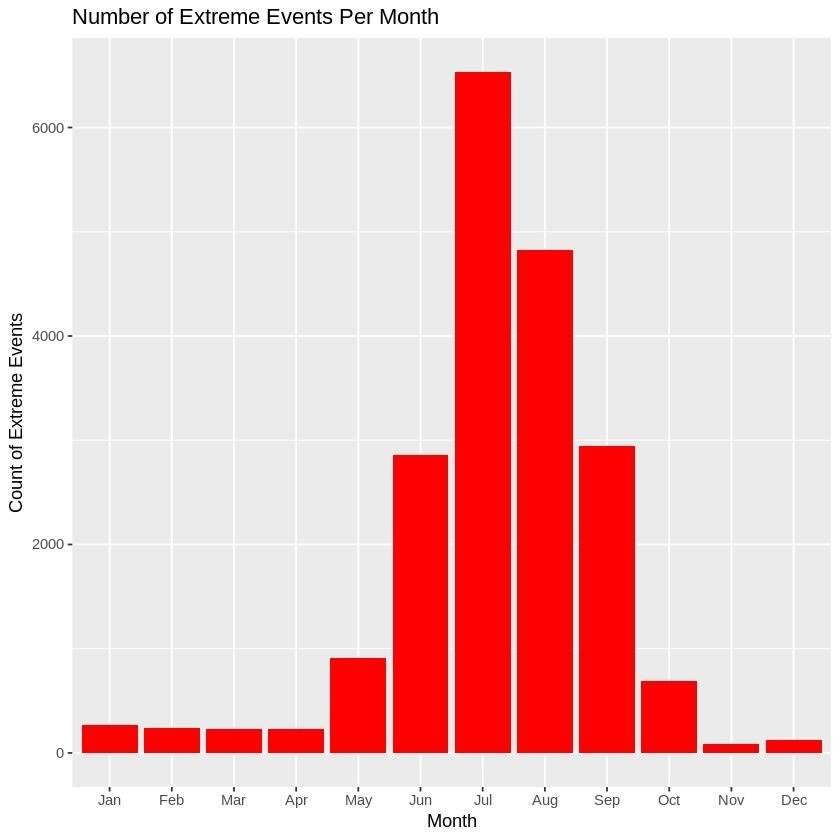
\includegraphics[width=0.5\textwidth]{figures/extreme_hilly.jpg}
    \caption{Number of Extreme Precipitation Events Per Month}
\end{figure}

\subsubsection*{Monthly Patterns}

\begin{itemize}
    \item Highest number of extreme events observed in July, followed by August and June.
    \item May and September show moderate activity—transitional monsoon months.
    \item Winter and spring months (November–April) show minimal extreme events.
\end{itemize}

\section*{Conclusion}

The analysis clearly highlights both a temporal increase in extreme rainfall events over the years and a strong seasonal concentration during the monsoon months. These findings emphasize the need for targeted flood preparation strategies, especially from June to September, and call for continuous monitoring and adaptation planning to improve climate resilience in vulnerable regions.


\section{Western Region Climate Data Analysis}

This analysis shows the temperature distribution across districts in the Western region of Nepal using spatial data visualization.

\subsection*{Filtering Districts}

\begin{verbatim}
# List of districts to match
district_list <- c("Gorkha", "Kaski", "Lamjung", "Manang", "Syangja",
                   "Arghakhanchi", "Gulmi",
                   "Nawalparasi", "Palpa", "Rupandehi", "Baglung",
                   "Myagdi", "Parbat","Mustang")

filtered_data_western <- df_climate[df_climate$District%in% district_list,]
\end{verbatim}

\subsection*{Geoplot for Temperature Distribution in Western Region}

\begin{verbatim}
# Calculate average temperature per district
plot_western <- filtered_data_western %>%
  group_by(District) %>%
  summarise(
    avg_temp = mean(Temp_2m, na.rm = TRUE),
    Latitude = first(Latitude),
    Longitude = first(Longitude)
  )

# Merge temperature data with spatial data
nepal_temp_west <- left_join(nepal_districts, plot_western , by = "District")

# GeoplotPlot
ggplot(data = nepal_temp_west) +
geom_sf(aes(data = avg_temp), color = "black") +
geom_point(aes(x = Longitude, y = Latitude, color = avg_temp), 
  size = 4) +  # Points for avg_temp
geom_text(data = plot_western, aes(
  x = Longitude, 
  y = Latitude, 
  label = District),
  size = 1.5, vjust = -0.5, color = "black") +
scale_color_gradient(low = "yellow", high = "red") +  # Color scale
labs(
  title = "Temperature Map of Nepal", fill = "Temperature"
  ) +
theme_minimal()
\end{verbatim}

% Figure here-----------------------------
\begin{figure}[h]
    \centering
    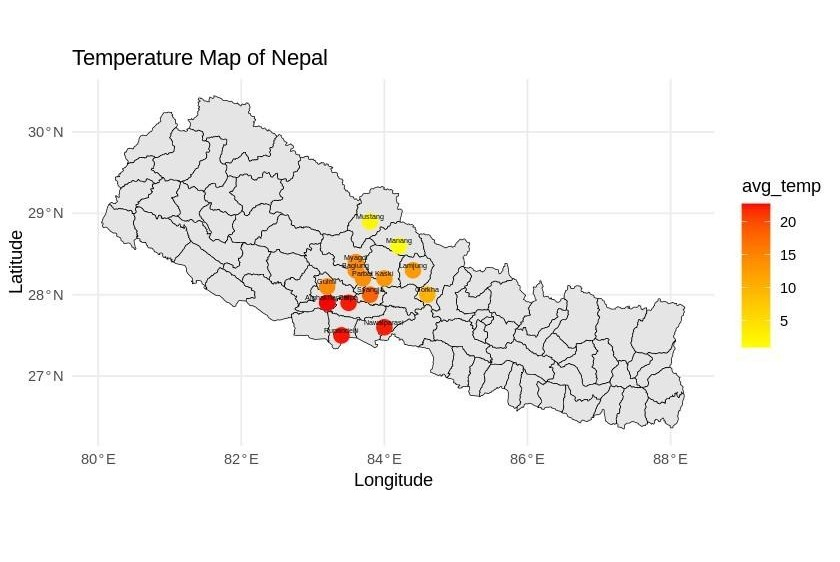
\includegraphics[width=0.6\textwidth]{figures/map_west.jpg}
    \caption{Temperature Map of Western Region}
\end{figure}

\subsection*{Scatter Plot of Temperature vs. Precipitation with Wind Speed by Season}

\begin{verbatim}
ggplot(filtered_data_western, aes(
  x = Temp_2m, 
  y = Precip, 
  color = Season, 
  size = WindSpeed_10m)) +
geom_point(alpha = 0.7) +
scale_color_manual(values = c(
    "Spring" = adjustcolor("yellow", alpha.f = 0.6),
    "Summer" = adjustcolor("red", alpha.f = 0.6),
    "Fall" = adjustcolor("orange", alpha.f = 0.6),
    "Winter" = adjustcolor("blue", alpha.f = 0.6)
  )) +
scale_size_continuous(range = c(1, 10)) +
labs(
title = "Scatter Plot of Temperature vs. Precipitation with Wind Speed Size",
x = "Temperature (°C)",
y = "Precipitation (mm/day)",
color = "Season",
size = "Wind Speed (10m)"
) +

theme_minimal()
\end{verbatim}

% Figure here-----------------------------
\begin{figure}[h]
    \centering
    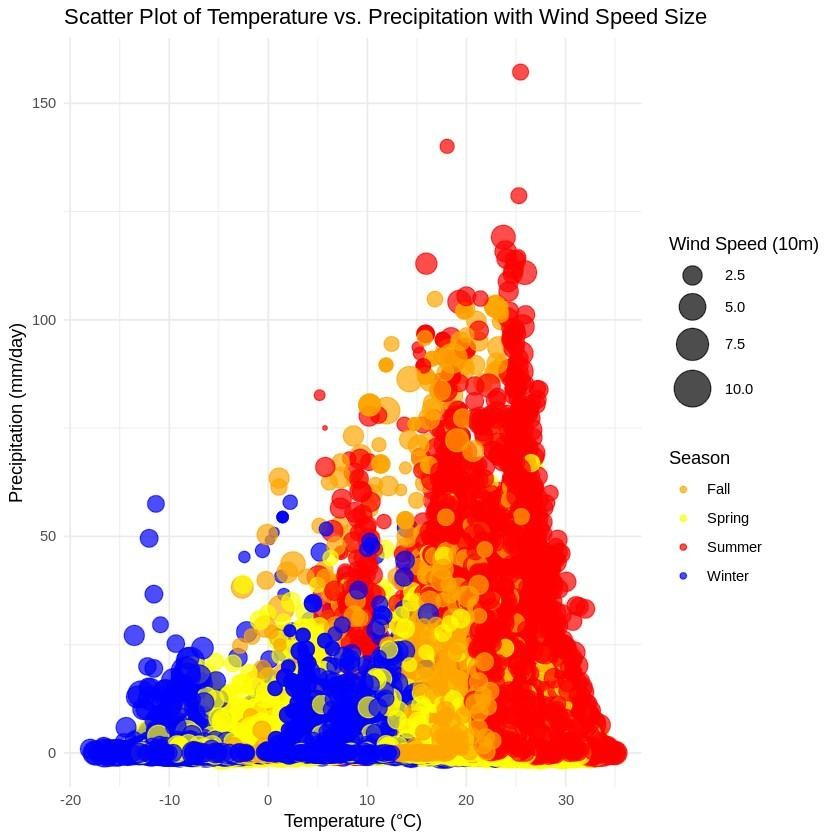
\includegraphics[width=0.5\textwidth]{figures/scatter_west.jpg}
    \caption{Scatterplot showing Temperature vs. Precipitation with Wind Speed by Season}
    \label{fig:scatter_temp_precip_wind}
\end{figure}

\subsection*{Histogram of Wind Speed with Density Curve for Western Region}

\begin{verbatim}
ggplot(filtered_data_western, aes(x = WindSpeed_10m)) +
geom_histogram(aes(y = ..density..), bins = 30, fill = "skyblue", 
color = "black", alpha = 0.7) + 
geom_density(color = "blue", linewidth = 1) + 
labs(
title = "Histogram of Wind Speed with Density Trendline for Western Region",
x = "Wind Speed (10m)",
y = "Density") +
theme_minimal()
\end{verbatim}

% Figure here-----------------------------
\begin{figure}[h]
    \centering
    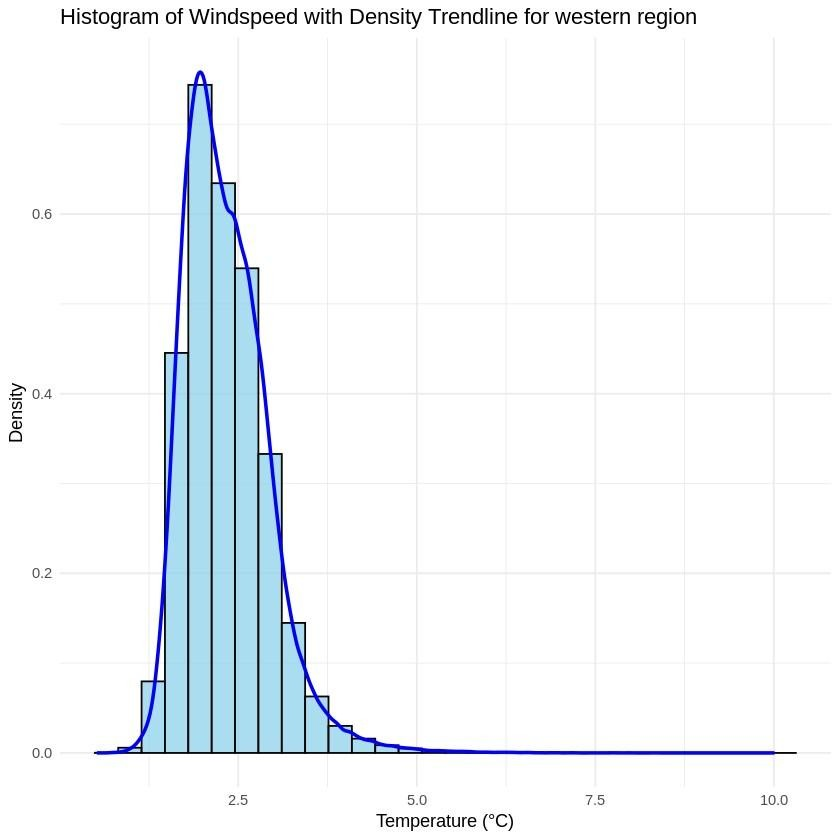
\includegraphics[width=0.5\textwidth]{figures/hist_west.jpg}
    \caption{Histogram of Wind Speed with Density Trendline for Western Region}
\end{figure}

\subsection*{Precipitation Trend Over Time in Western Region}

\begin{verbatim}
ggplot(filtered_data_western, 
aes(
  x = Date, 
  y = Precip)) +
geom_line(color = "blue") +
labs(
  title = "Precipitation Trend Over Time - Western Region",
  x = "Date", 
  y = "Precipitation (mm)") +

  theme_minimal()
\end{verbatim}

% Figure here--------------------------
\begin{figure}[h]
    \centering
    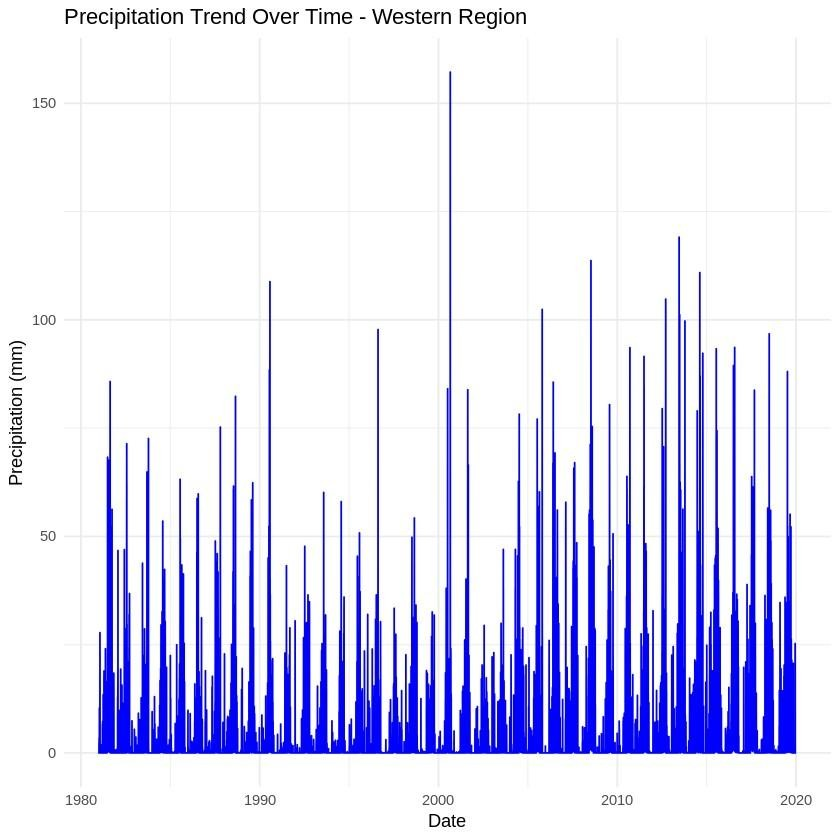
\includegraphics[width=0.5\textwidth]{figures/precip_west.jpg}
    \caption{Precipitation Trend Over Time - Western Region}
\end{figure}

\subsection*{Temperature Distribution by Season}

\begin{verbatim}
ggplot(filtered_data_western, aes(x = Season, y = Temp_2m, fill = Season)) +
  geom_boxplot() +
  labs(title = "Temperature Distribution by Season",
       x = "Season", y = "Temperature (°C)") +
  theme_minimal() +
  theme(legend.position = "none")
\end{verbatim}

% Figure here-----------------------------
\begin{figure}[h]
    \centering
    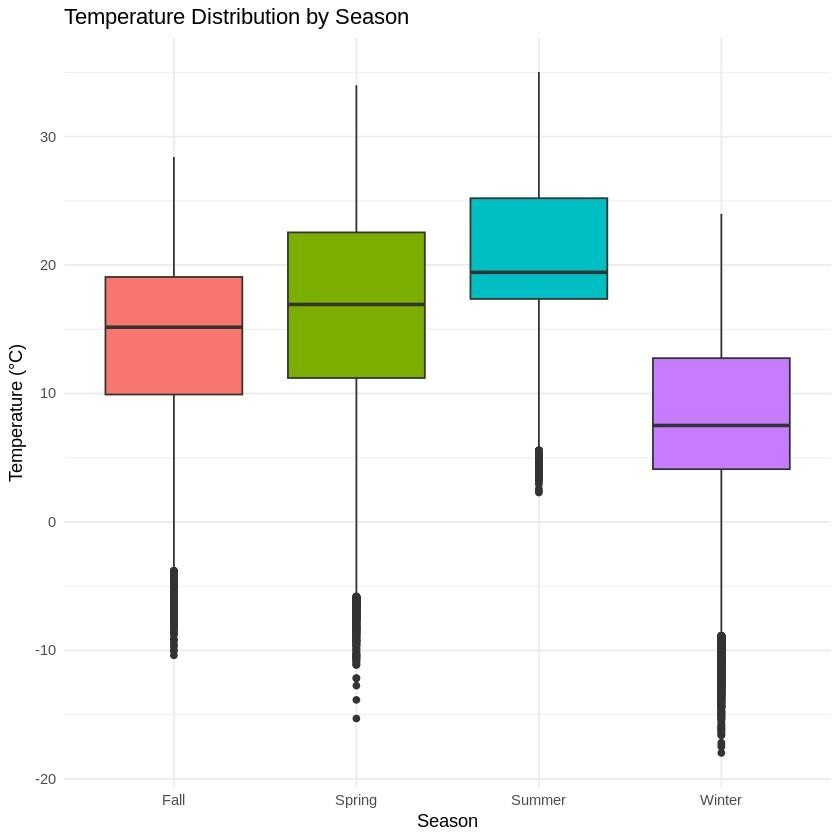
\includegraphics[width=0.5\textwidth]{figures/box_west.jpg}
    \caption{Temperature Distribution by Season in Western Region}
\end{figure}

\section{Time Based Data Analysis (May - August)}

This section filters data for the seasonal months of May through August and visualizes various climate variables including precipitation, humidity, temperature, wind speed, and their distributions.

\subsection*{Filtering Seasonal Months}

\begin{verbatim}
time_based_filter <- df_climate %>%
   dplyr::filter(Month_Label %in% c("May","Jun","Jul","Aug"))
dim(time_based_filter)
\end{verbatim}

\subsection*{Comparison of Precipitation and Humidity by Month}

\begin{verbatim}
precip_temp_data_long <- pivot_longer(precip_temp_data, 
cols = c(Avg_Precip, Avg_humid), 
names_to = "Variable", values_to = "Value")

ggplot(precip_temp_data_long, aes(x = Month_Label, y = Value, 
fill = Variable)) +
geom_bar(stat = "identity", position = "dodge") +
labs(
  title = "Comparison of Precipitation and Humidity by Month",     
  x = "Month", 
  y = "Value") +
  theme_minimal()
\end{verbatim}

% Figure here--------------------
\begin{figure}[h]
    \centering
    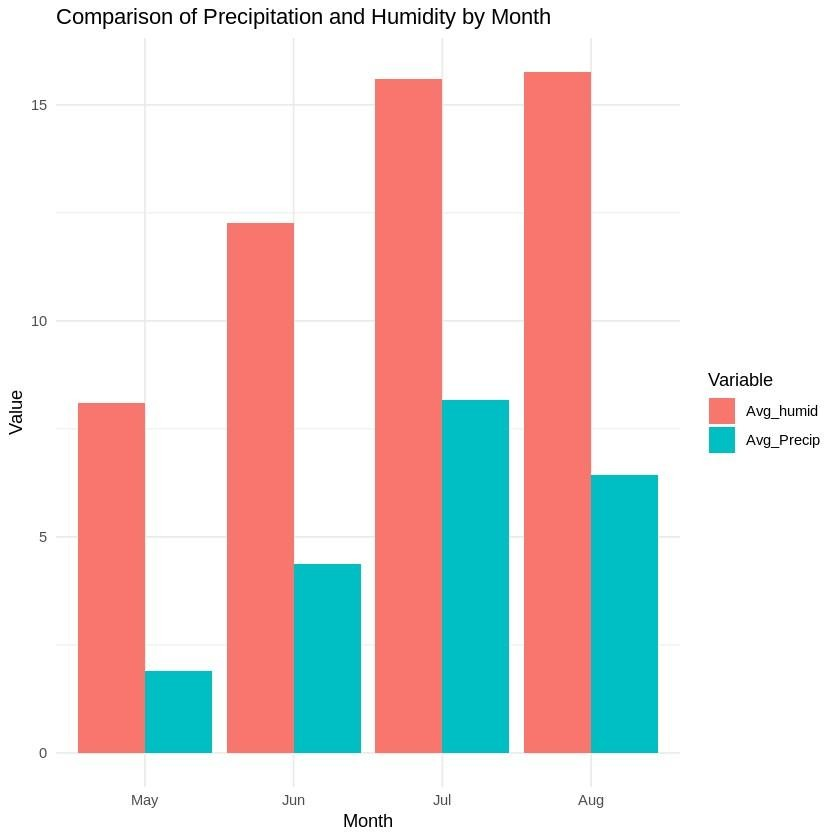
\includegraphics[width=0.5\textwidth]{figures/bar_time.jpg}
    \caption{Bar chart showing precipitation and humidity by month (May to August)}
\end{figure}

\subsection*{Relative Humidity vs Temperature for May to August}

\begin{verbatim}
ggplot(time_based_filter, aes(
  x = Temp_2m, 
  y = RH_2m)) +
geom_point(alpha = 0.3, color = "blue") +
labs(
    title = "Relative Humidity vs Temperature (May - Aug)",
    x = "Temperature (°C)", 
    y = "Relative Humidity (%)") +
  
theme_minimal()
\end{verbatim}

% Figure here-----------------------------
\begin{figure}[h]
    \centering
    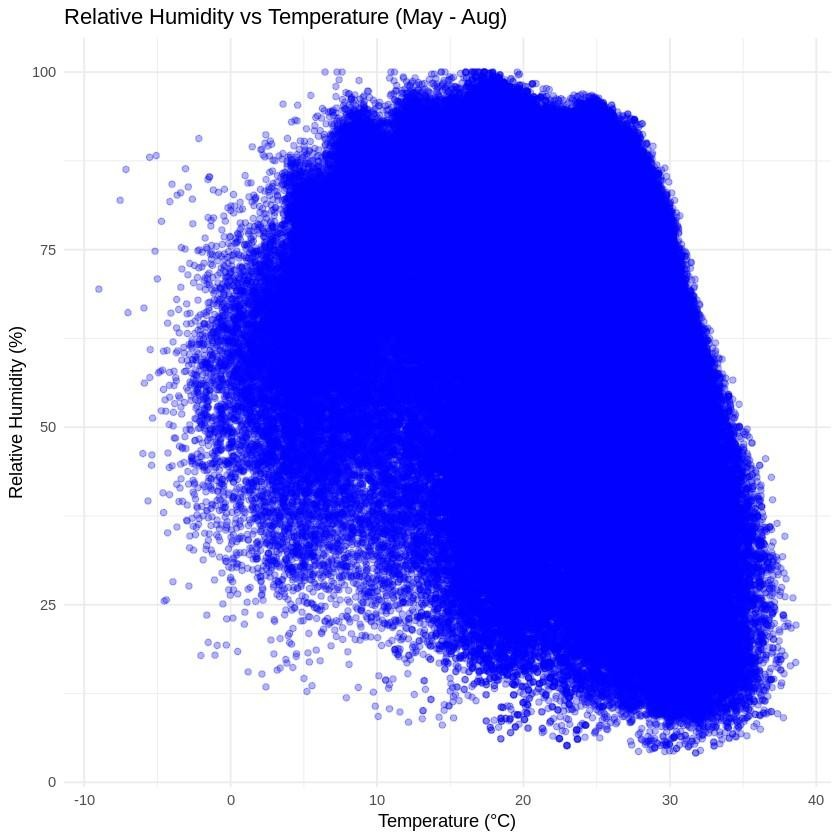
\includegraphics[width=0.5\textwidth]{figures/scatter_time.jpg}
    \caption{Scatterplot showing Temperature vs Relative Humidity (May to August)}
\end{figure}

\subsection*{Wind Speed Range at 10m by Month}

\begin{verbatim}
ggplot(time_based_filter, aes(
  x = Month_Label, 
  y = WindSpeedRange_10m, 
  fill = Month_Label)) +
geom_boxplot() +
labs(
  title = "Wind Speed Range at 10m by Month",
  x = "Month", 
  y = "Wind Speed Range (m/s)") +
  theme_minimal() +
  theme(legend.position = "none")
\end{verbatim}

\begin{figure}[h]
    \centering
    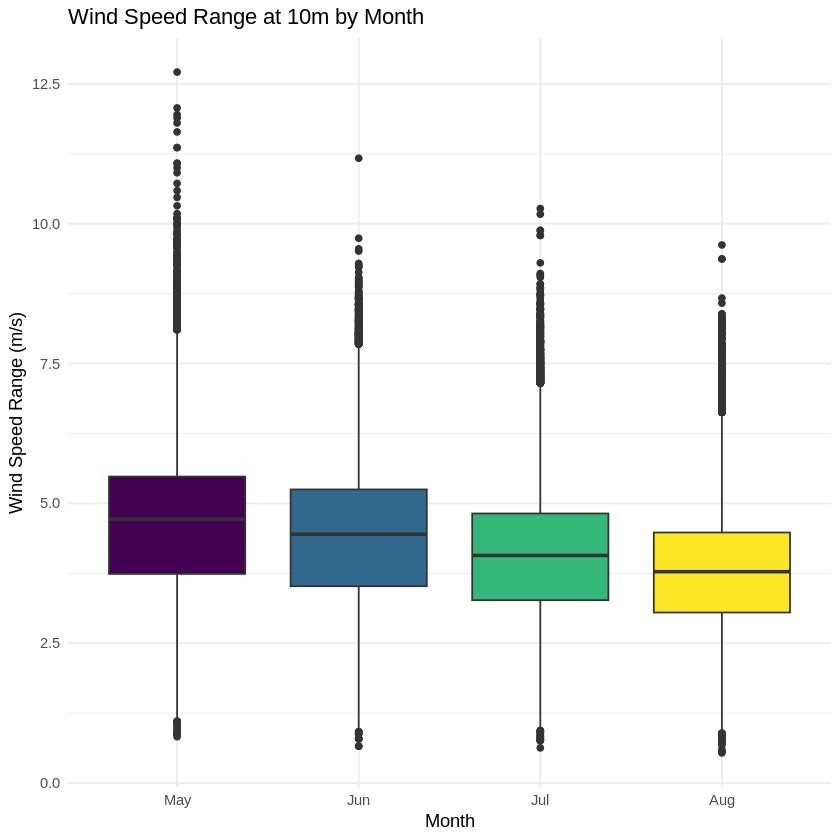
\includegraphics[width=0.5\textwidth]{figures/box_time.jpg}
    \caption{Boxplot of Wind Speed Range at 10m by Month (May to August)}
\end{figure}

\subsection*{Average Temperature Heatmap by District and Month}

To find out how temperature varies by district across different months, we created a heatmap that shows the average temperature for each district by month. This visualization helps us quickly identify seasonal patterns and regional differences in temperature across Nepal.
\begin{verbatim}
library(reshape2)

avg_temp_district <- time_based_filter %>%
  group_by(District, Month_Label) %>%
  summarise(
    AvgTemp = mean(Temp_2m, na.rm = TRUE)) %>%
  ungroup()

ggplot(avg_temp_district, aes(
  x = Month_Label, 
  y = District, 
  fill = AvgTemp)) +
  geom_tile() +
  scale_fill_viridis_c(option = "plasma") +
  labs(
    title = "Average Temperature by District and Month",
    x = "Month", 
    y = "District", 
    fill = "Avg Temp (°C)") +

  theme_minimal() +

  theme(axis.text.y = element_text(size = 6))
\end{verbatim}

% Figure here-----------------------------
\begin{figure}[h]
    \centering
    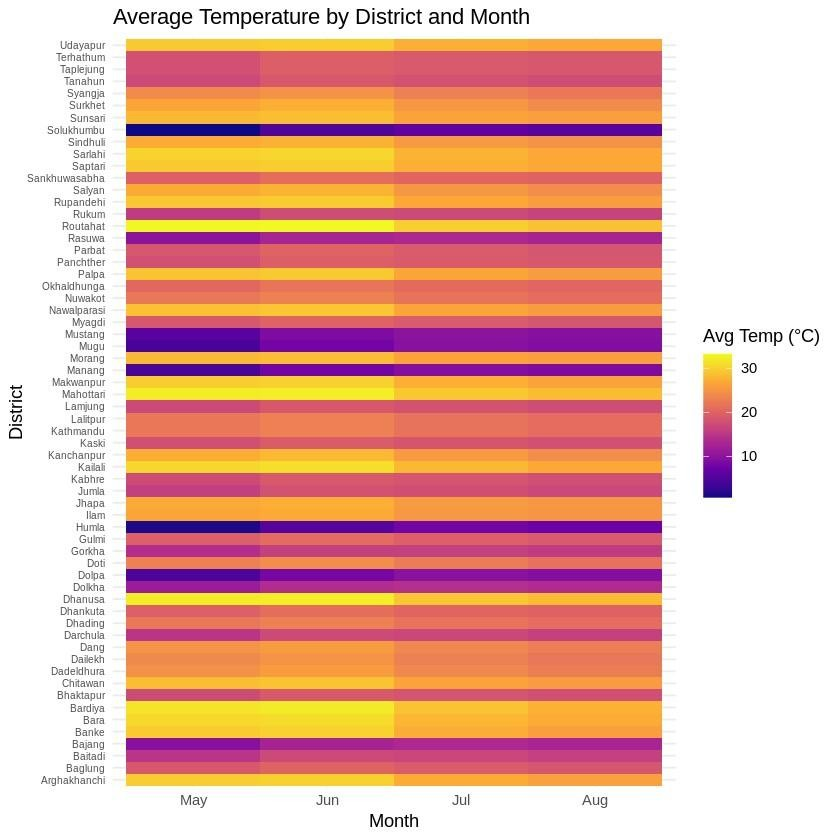
\includegraphics[width=0.6\textwidth]{figures/heatmap_time.jpg}
    \caption{Average Temperature Heatmap by District and Month (May to August)}
    \label{fig:avg_temp_heatmap}
\end{figure}

\subsection*{Density Plot of Temperature by Month}

\begin{verbatim}
ggplot(time_based_filter, aes(x = Temp_2m, fill = Month_Label)) +
  geom_density(alpha = 0.5) +
  labs(title = "Temperature Density by Month (May-August)",
       x = "Temperature (°C)", y = "Density") +
  theme_minimal()
\end{verbatim}

% Figure here------------------------
\begin{figure}[h]
    \centering
    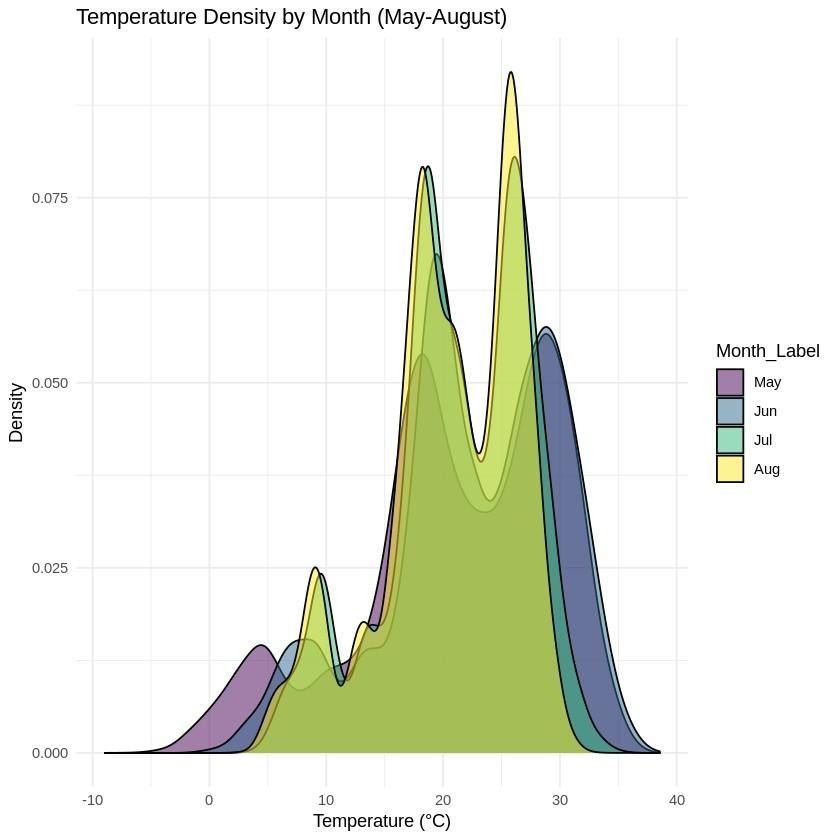
\includegraphics[width=0.45\textwidth]{figures/density_time.jpg}
    \caption{Density plot of Temperature distribution by month (May to August)}
    \label{fig:temp_density}
\end{figure}

\chapter{Merging with Agriculture Dataset}

Imagine you are a farmer or an agricultural planner trying to make the best decisions for the upcoming planting season. What if you could peek into the climate’s behavior — temperature changes, rainfall patterns, wind speed — and understand exactly how these factors affect crop growth?

In this chapter, we take a fascinating step forward: we merge agricultural data with climate data. By combining these two worlds, we can uncover deeper insights about how weather and climate influence agricultural productivity, helping farmers, scientists, and policymakers make smarter, data-driven decisions. Let’s think about this together:

\begin{itemize}
    \item How do you think temperature fluctuations affect crop yield?
    \item What role does rainfall play in the growth cycle of different crops?
    \item Can wind patterns influence soil erosion or pollination?
\end{itemize}

By the end of this chapter, you’ll not only learn how to merge these datasets technically, but also explore why this integration is so crucial for understanding the bigger picture of agriculture under changing climate conditions.

Ready to see the magic happen when data meets reality? Let’s dive in!

\subsection*{Sourcing Agricultural Data}
To carry out this integration, we sourced agricultural data from a publicly available interactive visualization platform: \\
\href{https://public.tableau.com/app/profile/sadichchha1369/viz/NepaCropMapwithprovinceSAMPLE_15636442141840/Dashboard1}{Tableau Public - Nepal Crop Map Dashboard}\\
This dataset includes district-level agricultural information, which we align with our climate dataset to explore temporal and spatial patterns in greater depth.
But before merging, let’s take a step back. Data, especially from real-world sources is rarely perfect. It often contains missing entries, inconsistent formats, or irrelevant information. That’s why our first task is to clean the agricultural dataset to ensure it aligns smoothly with our climate data.


\section{Data Preprocessing}

Data preprocessing is the process of preparing raw data for analysis by cleaning and transforming it into a usable format. In data mining it refers to preparing raw data for mining by performing tasks like cleaning, transforming, and organizing it into a format suitable for mining algorithms.

Goal is to improve the quality of the data, handling missing values, removing duplicates, and normalizing data to ensures the accuracy and consistency of the dataset.

\subsection{Data Cleaning}

In this step, we focus on cleaning the dataset to prepare it for analysis.

\begin{enumerate}
\item \textbf{Check For Null Values:}

We should identify any missing values across the dataset, and decide how to handle them (impute, drop, or analyze separately). For this particular dataset no null values were found.

\begin{verbatim}
sum(is.na(df_climate))
\end{verbatim}

\item\textbf{Drop the unnecessary columns:}

In our data set the first column consisting of an index is not necessary so we can drop the first unnamed column from our climate dataset.

\begin{verbatim}
df_climate$X <- NULL
\end{verbatim}

\item\textbf{Inspect the Duplicate Columns:}

We must also check for duplicate columns and remove them as they don't provide any additional information. For this particular climate dataset no such columns were found.

\begin{verbatim}
duplicated(colnames(df_climate))
\end{verbatim}

\item\textbf{Convert Date Column to Date Format:}

Since the Date column is currently in character format, convert it to Date using \texttt{as.Date()}.

\begin{verbatim}
df_climate$Date <- as.Date(df_climate$Date, format = "%Y-%m-%d")
\end{verbatim}

\item \textbf{Set Date as Index:}

Setting the date as an index is not strictly necessary in R for time series data analysis, but it is often a good practice and can simplify time-based operations. Setting the date as an index (or primary column) helps in slicing, filtering, and aggregating data by time periods. For this data set I used \texttt{tsibble} package.

\begin{verbatim}
# Convert tibble to tsibble
df_climate <- as_tsibble(df_climate, index = Date, key = District)

# Check for index
index_name <- index_var(df_climate)
print(index_name)
\end{verbatim}

The dataset structure after cleaning looks like:

\begin{verbatim}
glimpse(df_climate)
\end{verbatim}

% Figure here ---------------------------
\begin{figure}[h!]
    \centering
    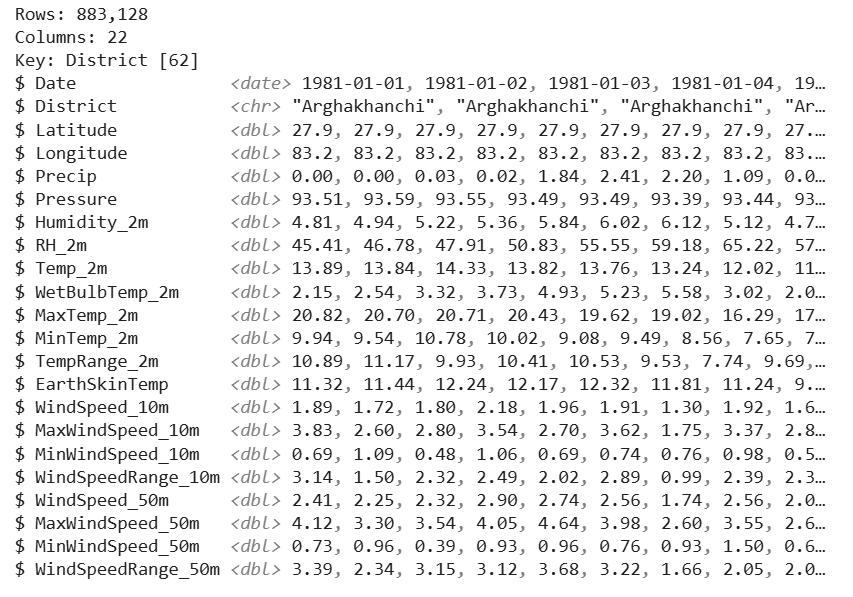
\includegraphics[width=0.6\textwidth]{figures/glimpse.png}
    \caption{Glimpse of the Cleaned Climate Dataset.}
\end{figure}

\end{enumerate}
\subsection{Feature Engineering}

Feature engineering is the process of taking raw data and transforming it into meaningful inputs that help a machine learning model understand patterns better. Think of it like preparing ingredients before cooking like when you chop, mix, and season them so the final dish tastes great.

In data analysis, this means creating new variables, cleaning data, selecting important information, or combining features to improve the model’s ability to make accurate predictions. Good feature engineering can often make a bigger difference in model performance than just using more complex algorithms.

It helps to create new features that might be helpful for your analysis. For this dataset, we can derive the month column from Date. Since Date is in format YYYY-MM-DD, we can extract the month and create a new column called month number. We can also create another column called month label and assign the names of the month (e.g., 1 = Jan, 2 = Feb, and so on).

\begin{verbatim}
# Extract month as number and label
df_climate$Month_Number <- month(df_climate$Date)     
df_climate$Month_Label <- month(df_climate$Date, label = TRUE)
\end{verbatim}

We can categorize the months into season and create a new column called “Season” for seasonal data analysis in the following way:

\begin{verbatim}
# Categorize months into seasons
df_climate <- df_climate %>%
  mutate(Season = case_when(
    month(Date) %in% c(12, 1, 2)  ~ "Winter",
    month(Date) %in% c(3, 4, 5)   ~ "Spring",
    month(Date) %in% c(6, 7, 8)   ~ "Summer",
    month(Date) %in% c(9, 10, 11) ~ "Fall"
  ))
\end{verbatim}

In R we can use \texttt{dplyr} and \texttt{lubridate} to extract the components of date. The function called \texttt{mutate()} can be used for creation of new columns and modifying the existing columns in our case.

\section{Merging Agriculture Data with Climate Data}

Previously, in the data slicing chapter, we created a subset of the climate dataset that includes only the districts classified as hilly regions. In this section, we will use this filtered climate data to merge with the agriculture dataset and perform agricultural analysis focused on the hilly region.

\subsection*{Filtering Hilly Region Data}
We first create a vector containing the list of districts in the hilly region:

\begin{verbatim}
districts_to_filter <- c("Arghakhanchi", "Baglung", "Baitadi", "Bhaktapur",
"Chitwan", "Dadeldhura", "Dailekh", "Dhading","Dhankuta", "Dolpa","Gorkha",
"Gulmi", "Ilam", "Jumla", "Kabhre", "Kaski", "Kathmandu", "Lalitpur",
"Lamjung", "Makwanpur", "Myagdi", "Nuwakot","Okhaldhunga","Palpa","Parbat",
"Rukum", "Salyan", "Sindhuli", "Surkhet", "Syangja")
\end{verbatim}

Then, we filter the climate dataset to include only the records corresponding to these districts:

\begin{verbatim}
filtered_hilly_data <- subset(df_climate, District %in% districts_to_filter)
\end{verbatim}

\subsection*{Extracting the Year from the Date Column}
Before merging the datasets, we need to extract the \texttt{Year} from the \texttt{Date} column in the filtered climate data:

\begin{verbatim}
filtered_hilly_data$Year <- year(filtered_hilly_data$Date)
\end{verbatim}

\subsection*{Saving the Filtered Dataset}
After filtering and extracting the year, we save the filtered dataset as a CSV file for future use:

\begin{verbatim}
write.csv(filtered_hilly_data,row.names = FALSE,file ="dataframe_hilly.csv")
\end{verbatim}

\subsection*{Merge Criteria}
To ensure proper alignment of the datasets, we merge them based on the following common identifiers:
\begin{itemize}
    \item \textbf{District:} The administrative region where both agricultural and climate data were recorded.
    \item \textbf{Year:} The calendar year of the recorded observations.
\end{itemize}

\subsection*{Merging the Datasets}
We merge the agricultural dataset \texttt{data\_agri\_clean} with the filtered hilly region climate dataset \texttt{filtered\_hilly\_data} based on the common identifiers:

\begin{verbatim}
merged_data <- merge(data_agri_clean, filtered_hilly_data, 
by = c("District", "Year"), all = FALSE) 
\end{verbatim}

This command performs an inner join, ensuring that only records with matching \texttt{District} and \texttt{Year} from both datasets are retained.

\section{Data Analysis and Visualization}

\subsection*{Identifying Major Crops in Hilly Regions}

This section identifies the main crops grown in Nepal’s hilly districts. By merging the cleaned agriculture and climate datasets, we analyze total crop production over time. Grouping by crop and summing production across years helps highlight the most widely produced crops in these regions.


\begin{verbatim}
top_crops <- merged_data %>%
  group_by(Crop) %>%
  summarise(Total_Production = sum(Production, na.rm = TRUE)) %>%
  arrange(desc(Total_Production))
ggplot(head(top_crops, 10), aes(
  x = Total_Production,y = reorder(Crop, Total_Production) )) +
geom_col(fill = "steelblue") + coord_flip() +
labs(title = "Top 10 Crops by Total Production in Hilly Regions",
x = "Crop", y = "Total Production")
\end{verbatim}

% Figure here-----------------------------
\begin{figure}[h]
\centering
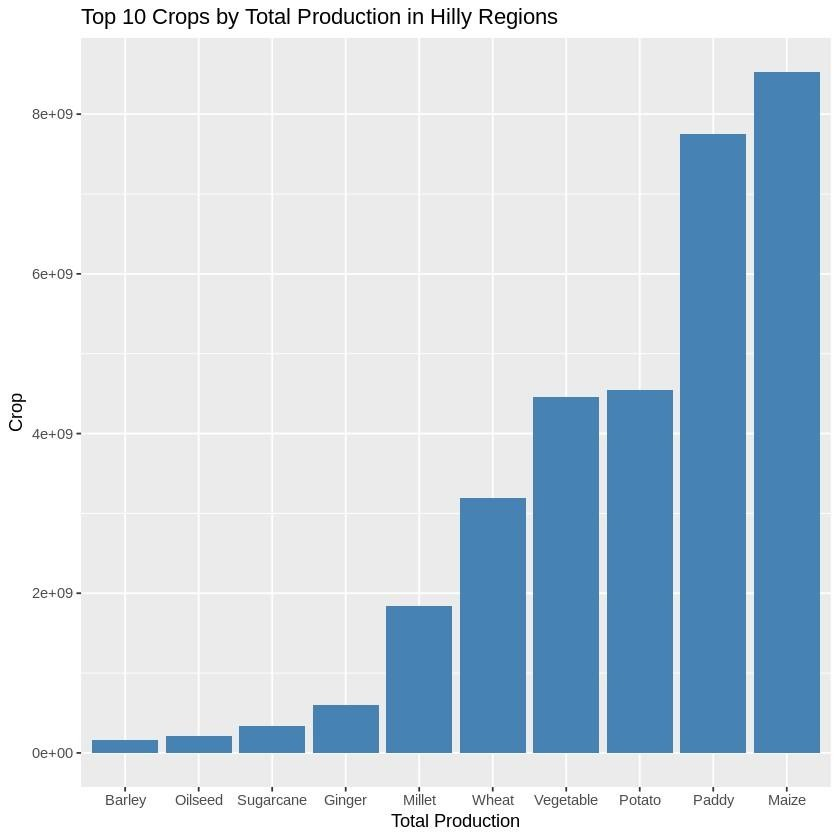
\includegraphics[width=0.5\textwidth]{figures/bar_agri.jpg}
\caption{ Top 10 Crops by Total Production in Hilly Region}
\end{figure}

The resulting plot clearly highlights the dominant crops cultivated in Nepal’s hilly regions. This insight is particularly valuable for stakeholders aiming to understand regional agricultural strengths or to design policies that support the most productive crops in these areas. Maize and Paddy are highly cultivated compared to others in hilly region.

\subparagraph*{Visualization of Agricultural Production by Crop Type in Hilly Districts
}
To understand the overall composition of agricultural production in the hilly districts, we visualize how different crop types contribute to production across various districts. This is done using a stacked bar chart, where each bar represents a district, and the stacked segments represent crop types.

\begin{verbatim}
ggplot(merged_data, aes(x = District, y = Production, fill = Crop.Type)) +
  geom_bar(stat = "identity", position = "stack") +
  coord_flip()
\end{verbatim}

% Figure here-----------------------------
\begin{figure}[h]
\centering
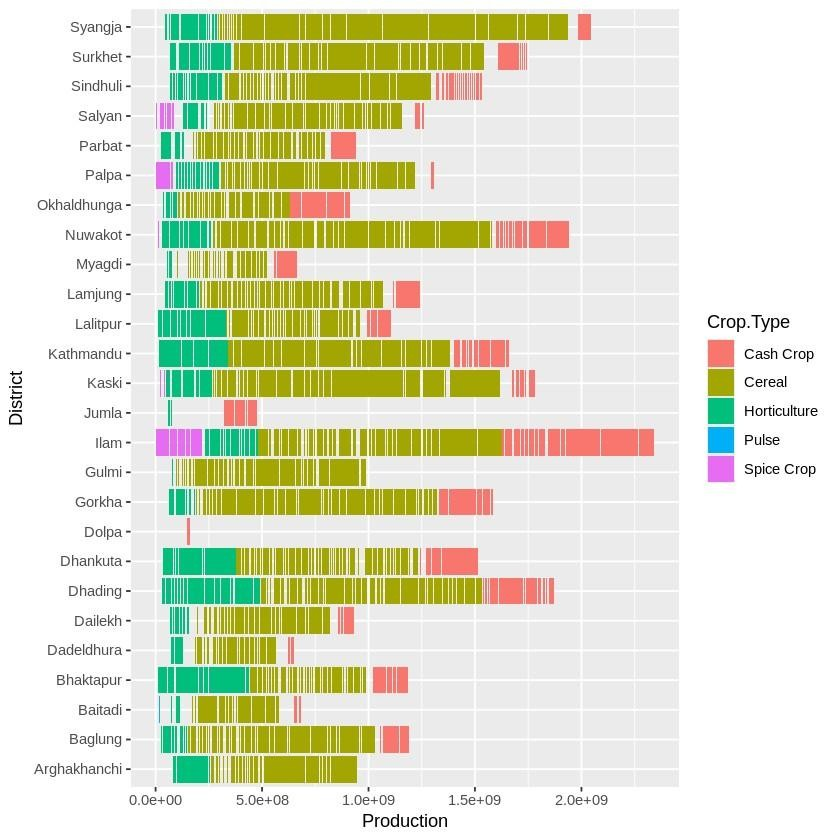
\includegraphics[width=0.6\textwidth]{figures/stacked_agri.jpg}
\caption{Stacked Barchart with crop type production in different districts}
\end{figure}

This visualization helps us compare which crop types dominate production in each district, and whether some regions have a more diverse agricultural profile than others. From the chart we can we that cereal production is highly dominating over hilly region.

\subsection*{Trend Analysis Over Time for Top 5 Crops}

To analyze how production of the most significant crops has changed over time in the hilly regions, we summarize and visualize the yearly production trends for the top 5 crops.

\begin{verbatim}
# Summarize yearly production for top crops
top_crops_list <- head(top_crops$Crop, 5)  # top 5 crops
yearly_trends <- merged_data %>%
  filter(Crop %in% top_crops_list) %>%
  group_by(Year, Crop) %>%
  summarise(Yearly_Production = sum(Production, na.rm = TRUE))
# Plot
ggplot(yearly_trends, aes(x = Year, y = Yearly_Production, color = Crop)) +
  geom_line(linewidth = 1) +
  labs(title = "Yearly Production Trends for Top Crops in Hilly Regions",
       x = "Year",
       y = "Production") +
  theme_minimal()
\end{verbatim}

% Figure here-----------------------------
\begin{figure}[h]
\centering
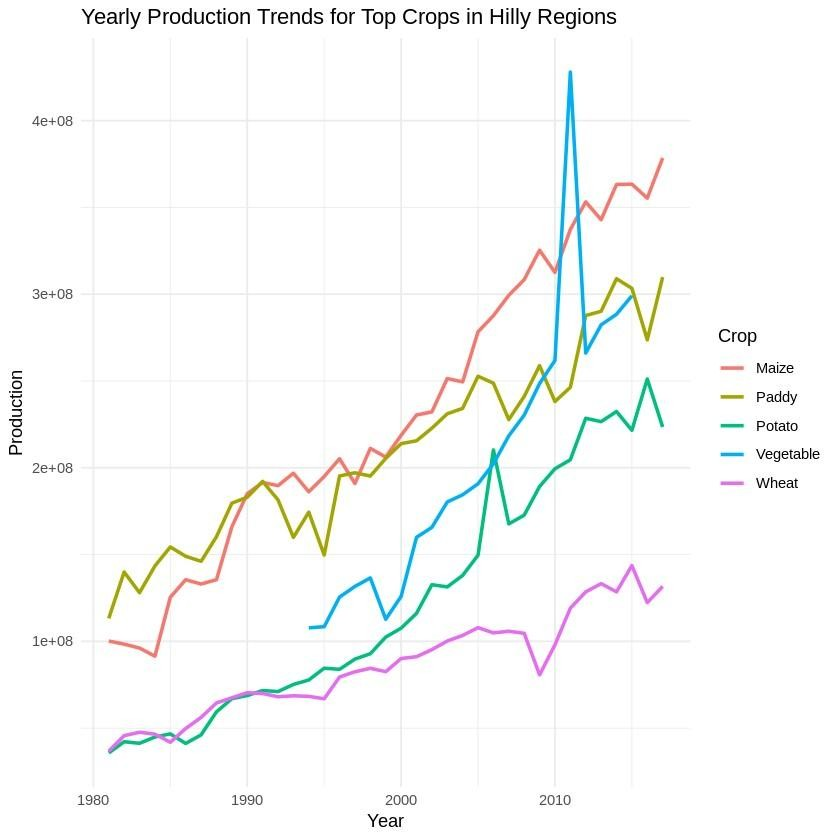
\includegraphics[width=0.5\textwidth]{figures/top5_agri.jpg}
\caption{Trend analysis of Top 5 crops in Hilly}
\end{figure}

\subsection*{Yearly Production of Paddy and Precipitation Trend}

To explore the relationship between agricultural production and climate, we analyze the yearly production of Paddy alongside average precipitation. The following R code aggregates yearly Paddy production and climate data, then plots them with dual y-axes to visualize trends concurrently.

\begin{verbatim}
# Assuming df_paddy_yearly is already created:
df_paddy_yearly <- merged_data %>%
  filter(Crop == "Paddy") %>%
  group_by(Year) %>%
  summarise(
    total_production = sum(Production, na.rm = TRUE),
    avg_temperature = mean(Temp_2m, na.rm = TRUE),
    avg_precip = mean(Precip, na.rm = TRUE)
  )


# Get the max values for dynamic scaling
max_prod_val <- max(df_paddy_yearly$total_production, na.rm = TRUE)
max_precip_val <- max(df_paddy_yearly$avg_precip, na.rm = TRUE)


target_max_proportion <- 0.7


ggplot(df_paddy_yearly, aes(x = Year)) +
  # Line and points for Production
geom_line(aes(y = total_production, color = "Total Production (Kg)"), 
linewidth = 1.2) +
geom_point(aes(y = total_production, color = "Total Production (Kg)"),
size = 3) +

# Line for Precipitation, scaled using the adjusted proportion
geom_line(aes(
  y = avg_precip * (target_max_proportion * max_prod_val / max_precip_val),
  color = "Average Precipitation (mm)"), linewidth = 1.2) +


# Add second axis for Precipitation, using the inverse of the adjusted scaling
scale_y_continuous(
  name = "Total Production (Kg)",
  sec.axis = sec_axis(~ . * (max_precip_val /
   (target_max_proportion * max_prod_val)),name = "Average Precipitation (mm)")
  ) +
# Manually set colors for the lines and define legend labels
scale_color_manual(
  name = "Variable",
  values = c(
      "Total Production (Kg)" = "darkgreen",
      "Average Precipitation (mm)" = "red"
    )
) +
# Titles and labels
labs(
    title = "Yearly Production of Paddy with Precipitation Trend",
    x = "Year"
  ) +
theme_minimal() +
theme(
    axis.text.x = element_text(angle = 45, hjust = 1),
    axis.title.y.left = element_text(color = "darkgreen"),
    axis.title.y.right = element_text(color = "red"),
    legend.position = "bottom",
    legend.title = element_blank(),
    plot.title = element_text(hjust = 0.5, face = "bold")
  )
\end{verbatim}

% Figure here-----------------------------
\begin{figure}[h]
\centering
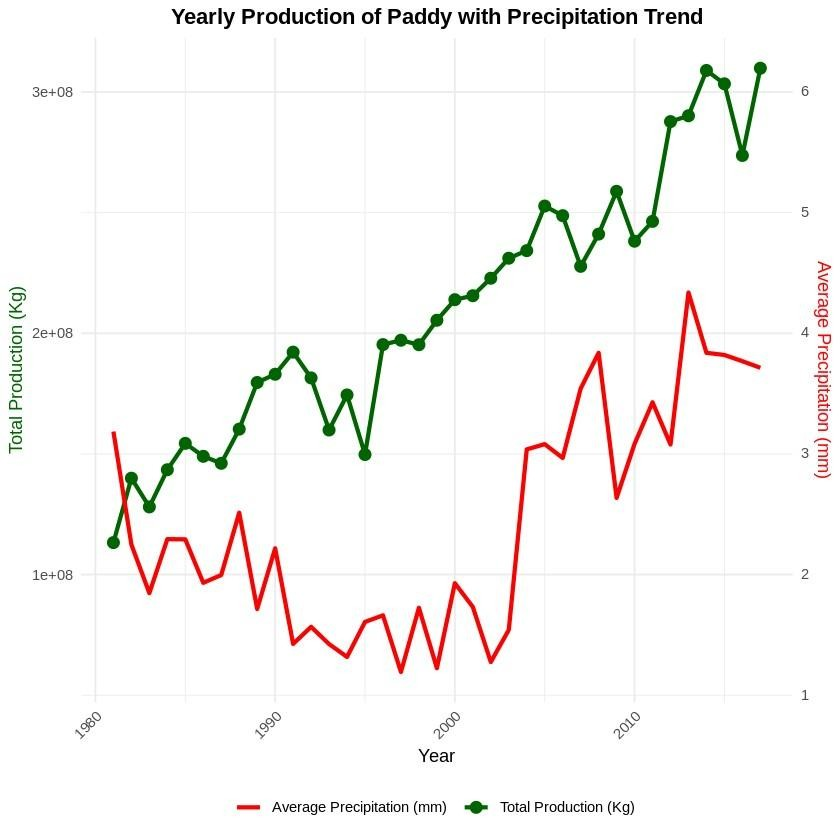
\includegraphics[width=0.5\textwidth]{figures/paddy_trend.jpg}
\caption{Yearly Production of Paddy and Precipitation Trend}
\end{figure}

This plot illustrates how Paddy production varies over the years alongside changes in average precipitation, providing insight into the dependency of agricultural yields on climatic factors in Nepal’s hilly regions. Paddy production has steadily increased over the years, but rainfall shows high variability. Notably, drops in rainfall often correspond to declines in paddy production, highlighting the critical role of adequate rainfall for consistent harvests despite improvements in farming practices.

\subsection*{Correlation Heatmap}

To better understand how climatic factors relate to agricultural outcomes such as crop yield and production, we analyze the correlations between key climate variables and agricultural metrics. This helps reveal any direct linear relationships and the strength of connections within the climate variables themselves. The following code computes and visualizes these correlations using a heatmap.

\begin{verbatim}
library(dplyr)
library(corrplot)
# Step 1: Create a clean numeric dataset for correlation
climate_agri_subset <- aggregated_data %>%
select(avg_temperature, avg_precip, avg_humidity, avg_pressure, avg_wind,
Yield, Production)

# Step 2: Compute correlation matrix
cor_matrix <- cor(climate_agri_subset, use = "complete.obs")

# Step 3: Visualize using corrplot
corrplot(cor_matrix, method = "color",
         type = "upper",        # Only upper triangle
         tl.col = "black",      # Text label color
         addCoef.col = "black", # Add correlation values
         number.cex = 0.7,      # Size of numbers
         col = colorRampPalette(c("red", "white", "blue"))(200))
\end{verbatim}

% Figure here-----------------------------
\begin{figure}[h]
\centering
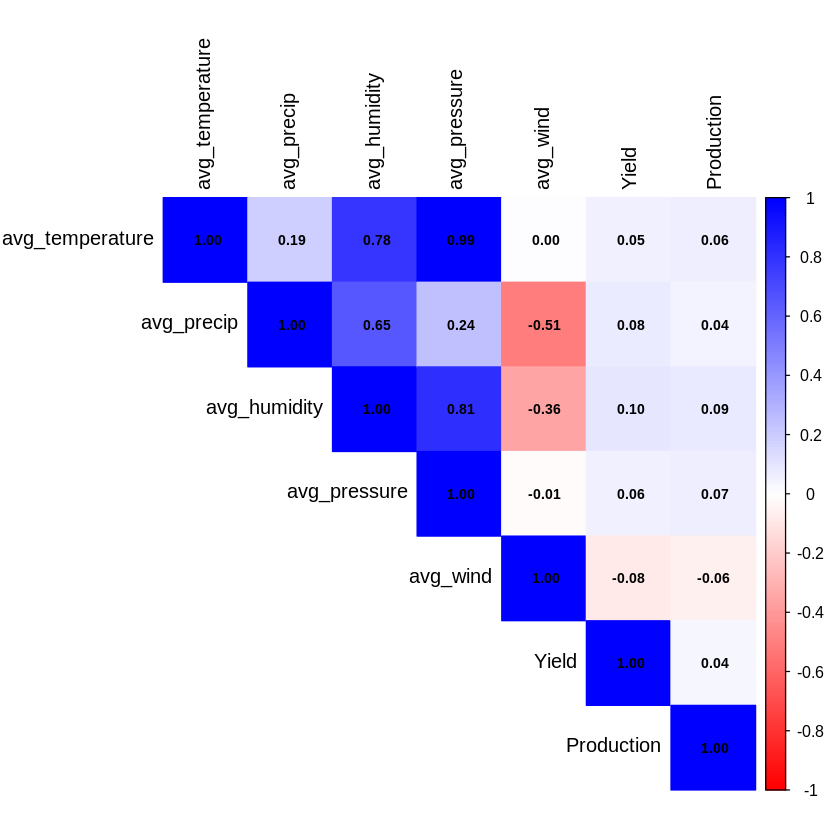
\includegraphics[width=0.5\textwidth]{figures/corr_agri.png}
\caption{Correlation Analysis}
\end{figure}

From this heatmap, several interesting points emerge:

\textbf{Weak Direct Link to Yield and Production:}  
  Correlations between Yield/Production and climate variables (temperature, precipitation, humidity, pressure, wind) are near zero, indicating little to no linear relationship at the annual average level.
  
 \textbf{Why This Matters:}  
 \begin{itemize}
  \item Linear correlation misses non-linear effects (e.g., too much or too little rain affecting yield).  
  \item Annual averages may mask critical seasonal or extreme weather impacts.  
  \item Other factors like technology or irrigation might overshadow climate effects.
 \end{itemize}

 \textbf{Strong Climate Variable Relationships:}  
 \begin{itemize}
  \item Temperature and Pressure: Nearly perfect positive correlation (0.99), suggesting redundancy.  
  \item Humidity: Positively correlated with temperature (0.78) and precipitation (0.65), reflecting natural atmospheric moisture dynamics.  
  \item Wind and Precipitation: Moderately negatively correlated (-0.51), meaning windy years tend to be drier.
 \end{itemize}





\chapter{Data Modeling}

As climate datasets grow in size and complexity, traditional descriptive methods are no longer sufficient to capture the full depth of information embedded within them. This is where advanced analytics plays a critical role.

Advanced analytics refers to a suite of statistical and computational techniques used to extract meaningful insights, detect hidden patterns, and build predictive models from data. In the context of climate science, these methods enable a deeper understanding of atmospheric behaviors, the ability to detect unusual events, and the development of models that can support forecasting and policy-making.

This section introduces powerful tools such as outlier detection, regression-based predictive modeling, and cluster analysis. These techniques move beyond exploration and visualization, allowing for the identification of climatic anomalies, prediction of future conditions, and classification of regions based on climatic similarities.

By integrating these advanced methods into climate analysis, researchers and practitioners can make more informed decisions, design better adaptation strategies, and contribute to a more resilient and sustainable future.

\section{Predictive Modeling – Linear Regression and Rainfall Forecasting}

Predictive modeling is a fundamental aspect of advanced data analytics. It involves using statistical techniques to forecast future values based on historical data. In the context of climate science, predictive models can be used to anticipate key environmental variables such as temperature, humidity, and precipitation.

One of the most commonly used predictive methods is regression analysis, which quantifies the relationship between a dependent variable and one or more independent variables. For example, we might use wind speed and humidity levels to predict rainfall amounts. By fitting a mathematical model to observed data, we can make informed projections about future conditions.

Predictive modeling in climate data offers several key benefits:
\begin{itemize}
  \item \textbf{Forecasting:} Provides estimations of future climate conditions, such as rainfall trends or temperature fluctuations.
  \item \textbf{Planning and Preparedness:} Supports agricultural planning, disaster risk reduction, and water resource management.
  \item \textbf{Insight into Variable Interactions:} Helps understand how different climatic factors influence one another.
\end{itemize}

In this chapter, we will:
\begin{itemize}
  \item Apply linear regression to model rainfall based on other climatic parameters.
  \item Interpret the model coefficients and assess the quality of predictions.
  \item Evaluate the model’s performance using statistical metrics.
\end{itemize}

This analytical approach enables a data-driven understanding of weather behavior, enhancing our ability to predict and prepare for changing climate scenarios.

\subsection*{Linear Regression Model Preparation and Evaluation}

In this section, we will build a linear regression model to predict precipitation based on two climatic parameters: temperature and humidity. This approach helps us understand how these variables contribute to rainfall patterns and allows us to make future predictions.

\subsubsection*{Step 1: Selecting the Variables}

We begin by selecting relevant variables from our dataset:

\begin{verbatim}
model_data <- climate_data %>%
  select(Temp_2m, Precip, Humidity_2m)
\end{verbatim}

\subsubsection*{Step 2: Fitting the Linear Regression Model}

We now fit a multiple linear regression model. The formula for the model is as follows:

\[
\text{Precipitation} = \beta_0 + \beta_1 \cdot \text{Temp\_2m} + \beta_2 \cdot \text{Humidity\_2m} + \epsilon
\]

Here, \(\beta_0\) is the intercept, \(\beta_1\) and \(\beta_2\) are the coefficients, and \(\epsilon\) represents the error term.

\begin{verbatim}
model <- lm(Precip ~ Temp_2m + Humidity_2m, data = model_data)
summary(model)
\end{verbatim}

The \texttt{summary(model)} function provides details about the coefficients and statistical significance of each variable, which help interpret how temperature and humidity influence precipitation.

\subsubsection*{Step 3: Making Predictions}

Using the fitted model, we generate predicted precipitation values:

\begin{verbatim}
predictions <- predict(model, newdata = model_data)
\end{verbatim}

% Figure here---------------------------
\begin{figure}[h]
\centering
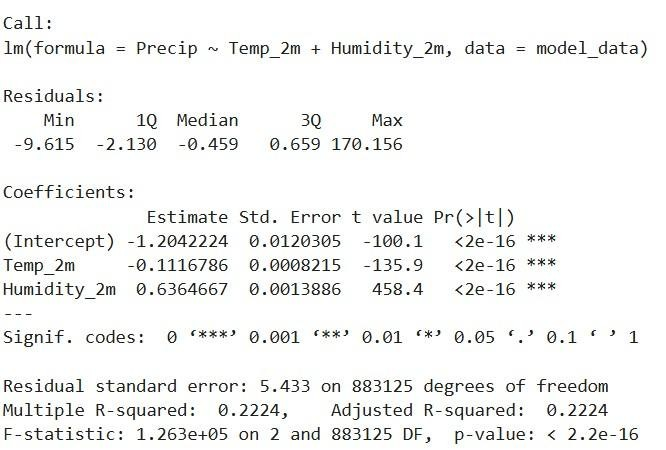
\includegraphics[width=0.6\textwidth]{figures/regression.jpg}
\caption{Model summary}
\end{figure}

\subsubsection*{Step 4: Model Evaluation}

To assess the model’s performance, we calculate:

\begin{itemize}
  \item \textbf{R-squared (R\(^2\))}: Measures how well the predictors explain the variance in the target variable. Values closer to 1 indicate a better fit.
  \item \textbf{Mean Squared Error (MSE)}: Measures the average squared difference between actual and predicted values. Lower MSE indicates better accuracy.
\end{itemize}

\begin{verbatim}
r_squared <- summary(model)$r.squared
mse <- mean((predictions - model_data$Precip)^2)

actual_avg <- mean(model_data$Precip)
predicted_avg <- mean(predictions)

cat("R-squared:", r_squared, "\n")
cat("Mean Squared Error (MSE):", mse, "\n")
cat("Actual Average Precipitation:", actual_avg, "\n")
cat("Predicted Average Precipitation:", predicted_avg, "\n")
\end{verbatim}

% Figure here-----------------------------
\begin{figure}[h]
\centering
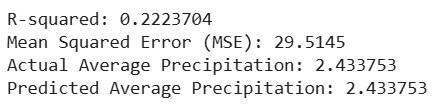
\includegraphics[width=0.5\textwidth]{figures/r_square.jpg}
\caption{Model evaluation metrics}
\end{figure}

\subsubsection*{Step 5: Visualizing Model Performance}

\textbf{Actual vs Predicted Plot:} This scatter plot compares the real precipitation values against the model’s predictions. The red line (y = x) indicates perfect prediction. Points close to this line show accurate predictions.

\begin{verbatim}
plot(model_data$Precip, predictions,
     xlab = "Actual Precipitation",
     ylab = "Predicted Precipitation",
     main = "Actual vs Predicted Precipitation")
abline(0, 1, col = "red")
\end{verbatim}

\textbf{Residual Plot:} This shows the residuals (errors) from the predictions. Ideally, residuals should be randomly scattered around zero. Patterns in residuals could suggest issues with the model fit.

\begin{verbatim}
residuals <- model$residuals
plot(residuals, main = "Residuals",
     ylab = "Residuals", xlab = "Index")
abline(h = 0, col = "red")
\end{verbatim}

% Figure here----------------------------
\begin{figure}[h]
\centering
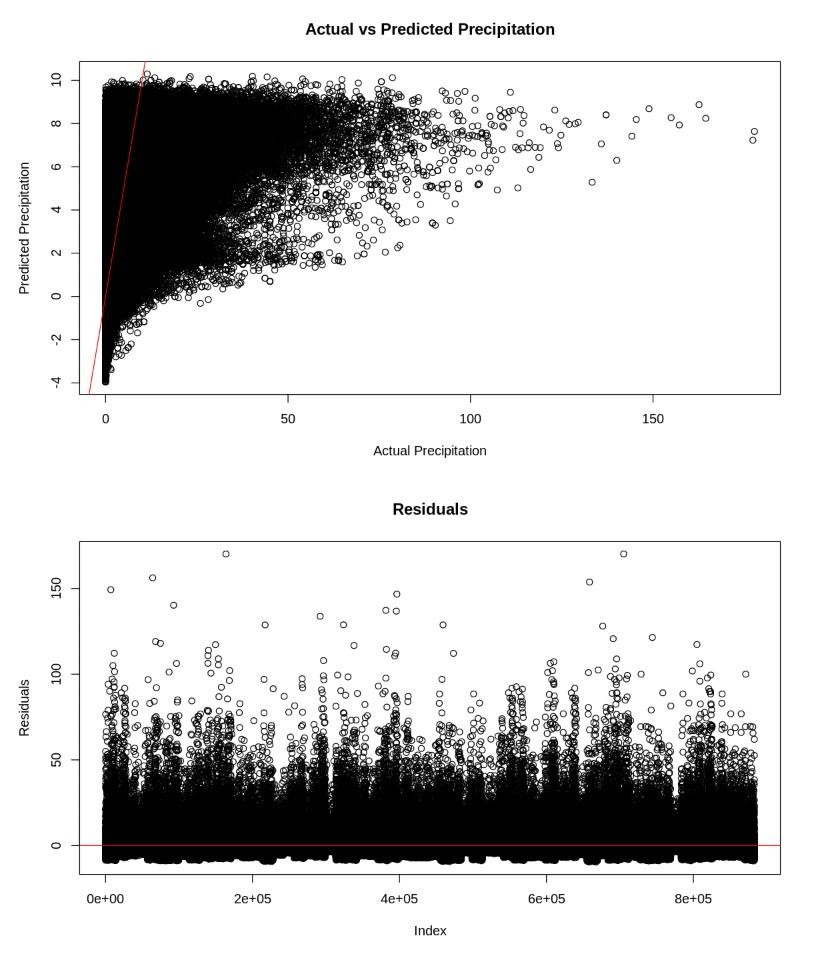
\includegraphics[width=0.5\textwidth]{figures/pred_residual.jpg}
\caption{Actual vs Predicted Plot and Residual Plot}
\end{figure}

\subsection*{Conclusion}

Through this exercise, we’ve seen how a simple regression model can be applied to climate data. We evaluated the model’s effectiveness using statistical metrics and visualizations, which are essential for interpreting the reliability and accuracy of predictions. As you explore more advanced models, this foundational approach will remain a critical tool for climate data analysis.
\clearpage

\subsection*{Predicting the Likelihood of Rainfall Based on Temperature and Humidity}

In this section, we’ll build a logistic regression model to predict whether rainfall will occur, using temperature and humidity as predictors. Instead of predicting how much rain will fall, we simplify the problem into a binary classification: Did it rain or not?

\subsubsection*{Step 1: Preparing the Data}

We start by creating a new variable in our dataset called \textit{Rain Occurrence}. This variable holds:

\begin{itemize}
  \item 1 if precipitation is greater than 0mm (indicating it rained)
  \item 0 otherwise (indicating no rain).
\end{itemize}

\begin{verbatim}
rain_data <- climate_data %>%
  mutate(Rain_Occurrence = ifelse(Precip > 0, 1, 0)) %>%
  select(Temp_2m, Humidity_2m, Rain_Occurrence)
\end{verbatim}

\subsubsection*{Step 2: Splitting the Dataset}

We divide our data into two parts:

\begin{itemize}
  \item \textbf{Training Set (80\%):} Used to train the model.
  \item \textbf{Testing Set (20\%):} Used to evaluate model performance.
\end{itemize}

\begin{verbatim}
set.seed(123)
train_index <- createDataPartition(rain_data$Rain_Occurrence, p = 0.8, 
list = FALSE)
train_data <- rain_data[train_index, ]
test_data <- rain_data[-train_index, ]
\end{verbatim}

\subsubsection*{Step 3: Standardizing the Features}

Before training, we standardize the temperature and humidity values to have a mean of 0 and a standard deviation of 1. This ensures that all features contribute equally to the model.

\begin{verbatim}
preprocess <- preProcess(train_data[, c("Temp_2m", "Humidity_2m")], 
method = c("center", "scale"))
train_data[, c("Temp_2m", "Humidity_2m")] <- predict(preprocess, 
train_data[, c("Temp_2m", "Humidity_2m")])
test_data[, c("Temp_2m", "Humidity_2m")] <- predict(preprocess, 
test_data[, c("Temp_2m", "Humidity_2m")])
\end{verbatim}

\subsubsection*{Step 4: Training the Logistic Regression Model}

We now fit a logistic regression model. This model estimates the probability of rain occurring based on the input temperature and humidity.

\begin{verbatim}
logistic_model <- glm(Rain_Occurrence ~ Temp_2m + Humidity_2m,
                      data = train_data, family = "binomial")
\end{verbatim}

\subsubsection*{Step 5: Making Predictions}

Once the model is trained, we make predictions on the test data:

\begin{itemize}
  \item Predicted Probability: the probability that rain will occur.
  \item Predicted Class: the classification (1 = rain, 0 = no rain) based on a threshold of 0.5.
\end{itemize}

\begin{verbatim}
test_data$Predicted_Prob <- predict(logistic_model, test_data,
type = "response")
test_data$Predicted_Class <- ifelse(test_data$Predicted_Prob > 0.5, 1, 0)
\end{verbatim}

\subsubsection*{Step 6: Evaluating the Model}

To assess the model’s effectiveness, we use a confusion matrix and compute several metrics:

\begin{itemize}
  \item \textbf{Accuracy:} Proportion of total correct predictions.
  \item \textbf{Precision:} Out of the times the model predicted rain, how often it was correct.
  \item \textbf{Recall (Sensitivity):} Out of the actual rainy instances, how many were correctly predicted.
  \item \textbf{F1-score:} Harmonic mean of precision and recall.
\end{itemize}

\begin{verbatim}
conf_matrix <- confusionMatrix(as.factor(test_data$Predicted_Class),
                               as.factor(test_data$Rain_Occurrence))

accuracy <- conf_matrix$overall["Accuracy"]
precision <- conf_matrix$byClass["Precision"]
recall <- conf_matrix$byClass["Recall"]
f1_score <- 2 * ((precision * recall) / (precision + recall))

cat("Accuracy:", accuracy, "\n")
cat("Precision:", precision, "\n")
cat("Recall:", recall, "\n")
cat("F1 Score:", f1_score, "\n")
\end{verbatim}

% Figure here----------------------------
\begin{figure}[h]
\centering
\includegraphics[width=0.3\textwidth]{figures/eval_metrics.jpg}
\caption{Evaluation metrics}
\end{figure}

\subsubsection*{Step 7: Visualizing Performance with the ROC Curve}

The ROC (Receiver Operating Characteristic) curve helps us visualize how well the model distinguishes between rainy and non-rainy days. The curve plots:

\begin{itemize}
  \item True Positive Rate (Recall) on the y-axis,
  \item False Positive Rate on the x-axis.
\end{itemize}

A curve closer to the top-left corner indicates better performance.

\begin{verbatim}
roc_curve <- roc(test_data$Rain_Occurrence, test_data$Predicted_Prob)
ggroc(roc_curve) +
labs(
  title = "ROC Curve", 
  x = "False Positive Rate", y = "True Positive Rate") +
theme_minimal()
\end{verbatim}

% Figure here--------------------------
\begin{figure}[h]
\centering
\includegraphics[width=0.5\textwidth]{figures/ROC.jpg}
\caption{ROC curve}
\end{figure}

\subsection*{Conclusion}

This logistic regression model gives us a practical tool to estimate the probability of rainfall using just temperature and humidity. While the model is simple, it introduces key classification concepts and serves as a foundation for more complex predictive techniques in climate analytics.

\section{Understanding Decision Trees}

A decision tree is one of the most intuitive and interpretable machine learning models used for both classification and regression tasks. In the context of climate analysis, decision trees help us understand how various atmospheric conditions contribute to an event such as heavy rainfall.


\subsection*{How Decision Trees Work}

A decision tree splits the dataset into branches based on the values of the input features. Each internal node represents a condition on a feature, and each leaf node represents an outcome.

The model continues to split the data into smaller groups to reduce uncertainty or “impurity.” In classification, a common measure for this impurity is the Gini Index or Entropy.

\begin{itemize}
  \item \textbf{Root Node:} The feature that best splits the data appears at the top.
  \item \textbf{Internal Nodes:} Represent decision rules based on features.
  \item \textbf{Leaf Nodes:} Represent class labels (e.g., 0 = No Heavy Rainfall, 1 = Heavy Rainfall).
\end{itemize}

\subsection*{Why Use Decision Trees in Climate Data?}

\begin{itemize}
  \item \textbf{Interpretability:} You can easily visualize and understand the rules that lead to predictions.
  \item \textbf{Non-linearity:} Trees can capture complex, non-linear interactions between variables.
  \item \textbf{No Need for Scaling:} Unlike many models, decision trees do not require feature standardization.
  \item \textbf{Handles Missing Values and Outliers:} Trees are robust to irregularities in the data.
\end{itemize}

\subsection*{Example Rule from the Tree}

Let’s say the decision tree discovers this rule: \\
If Humidity 2m $>$ 70 and Pressure $<$ 1010, then the model predicts Heavy Rainfall = 1.

This simple rule can help stakeholders quickly assess risk from available sensor readings.

\subsection*{Limitations of Decision Trees}

Despite their advantages, decision trees can overfit the training data if not carefully tuned. That means they may perform well on training data but poorly on unseen data. This can be mitigated by:

\begin{itemize}
  \item Pruning the tree (removing weak or unnecessary branches).
  \item Limiting the depth of the tree.
  \item Using ensemble methods (e.g., random forests or gradient boosting).
\end{itemize}

\subsection*{Visualizing the Tree Structure}

The tree diagram provides a clear representation of how the model splits the data and which features are most influential.

\begin{verbatim}
plot(tree_model)
text(tree_model, pretty = 0)
\end{verbatim}

This visualization not only shows the decision points but also helps explain the model’s logic to non-technical stakeholders, such as meteorologists or disaster management teams.

\subsection*{Classifying Heavy Rainfall Events Using Decision Trees}

To identify instances of heavy rainfall, we can use a decision tree model. In this section, we classify rainfall events as either Heavy or Not Heavy based on meteorological variables such as temperature, humidity, pressure, and wind speed.

We define a heavy rainfall event as one where precipitation exceeds the 75th percentile. The following R code demonstrates how to create and evaluate a decision tree model for this classification task.

\begin{verbatim}
# Install and load necessary package
install.packages("tree")
library(tree)
# Create a new column indicating heavy rainfall
precip_data <- climate_data %>%
  mutate(Heavy_Rainfall = ifelse(Precip > quantile(Precip, 0.75), 1, 0))
# Convert Heavy_Rainfall to factor for classification
precip_data$Heavy_Rainfall <- as.factor(precip_data$Heavy_Rainfall)
# Split data into training (80%) and testing (20%) sets
set.seed(123)
train_index <- createDataPartition(precip_data$Heavy_Rainfall, p = 0.8,
list = FALSE)
train_data <- precip_data[train_index, ]
test_data <- precip_data[-train_index, ]
# Train the decision tree model
tree_model <- tree(
Heavy_Rainfall ~ Temp_2m + Humidity_2m + Pressure + WindSpeed_10m, 
data = train_data)
# View summary of the model
summary(tree_model)
# Make predictions on test data
predictions <- predict(tree_model, test_data, type = "class")
# Evaluate the model using confusion matrix
conf_matrix <- table(Predicted = predictions, Actual = test_data$Heavy_Rainfall)
print(conf_matrix)
# Calculate performance metrics
accuracy <- sum(diag(conf_matrix)) / sum(conf_matrix)
precision <- conf_matrix[2, 2] / sum(conf_matrix[, 2])
recall <- conf_matrix[2, 2] / sum(conf_matrix[2, ])
f1_score <- 2 * (precision * recall) / (precision + recall)
# Print metrics
cat("Accuracy: ", accuracy, "\n")
cat("Precision: ", precision, "\n")
cat("Recall: ", recall, "\n")
cat("F1-score: ", f1_score, "\n")


\end{verbatim}

% Figure here---------------------------
\begin{figure}[h]
\centering
\includegraphics[width=0.5\textwidth]{figures/tree_summ.jpg}
\caption{Model summary}
\end{figure}

\begin{verbatim}
  # Visualize the decision tree
plot(tree_model)
text(tree_model, pretty = 0)
\end{verbatim}

% figure here----------------------------
\begin{figure}[h]
\centering
\includegraphics[width=0.5\textwidth]{figures/tree.jpg}
\caption{Classifying Heavy Rainfall Events Using Decision Trees}
\end{figure}

The decision tree model learns decision rules based on climate variables to classify whether a given observation is a heavy rainfall event.

The confusion matrix and the calculated performance metrics (accuracy, precision, recall, and F1-score) allow us to evaluate how well the model distinguishes between the two classes.

The visualization of the tree provides insight into which features most strongly influence the classification. This model can be improved or expanded by exploring ensemble techniques such as Random Forests or Gradient Boosting, which often provide more accurate and stable predictions.

\subsection*{Conclusion}

Decision trees offer a transparent and flexible way to classify rainfall events based on meteorological variables. When interpretability and ease of use are important, they can be an ideal choice in climate prediction applications.

\section{Cluster Analysis for Climatic Regions}

Cluster analysis is a powerful unsupervised machine learning technique used to identify natural groupings within data. In the context of climate science, cluster analysis helps uncover regions with similar climatic behavior, even when they may be geographically distant.

The idea is simple: group together climate observations that are more similar to each other than to those in other groups. This allows researchers and policymakers to:
\begin{itemize}
    \item Identify climate zones based on observed data (e.g., temperature, precipitation, humidity).
    \item Compare regional climate behaviors.
    \item Tailor climate adaptation strategies to similar zones.
\end{itemize}

\subsection*{How It Works}

Let’s say we have a dataset with climate measurements such as temperature, humidity, precipitation, and wind speed. Each row in our data represents a region or time-point, and our goal is to group these rows into “clusters” of similar climate patterns.

Key steps in the clustering process:
\begin{enumerate}
    \item \textbf{Feature Selection:} Choose the relevant variables (e.g., temperature, humidity).
    \item \textbf{Standardization:} Scale the variables so that each contributes equally to the clustering.
    \item \textbf{Choosing the Number of Clusters (K):} Decide how many climate groups to form using techniques like the elbow method.
    \item \textbf{Applying Clustering Algorithm:} Use algorithms like k-means to partition the data into K clusters.
    \item \textbf{Interpretation:} Analyze and visualize the clusters to understand regional patterns.
\end{enumerate}

\subsection*{Cluster Analysis for Climatic Patterns}

\textbf{Understanding the Goal}\\

Imagine you’re handed a huge table full of weather data with temperature, precipitation, humidity, and more from different regions or time periods. A natural question might arise: “Can we group these observations into meaningful climate categories?”

That’s where clustering helps. It automatically finds groups (called clusters) in your data that share similar features. Here, we want to find such clusters based on:
\begin{itemize}
    \item \texttt{Temp\_2m} – Temperature at 2 meters height
    \item \texttt{Precip} – Precipitation
\end{itemize}

\textbf{Step-by-Step Exploration}\\

\textbf{Step 1: Clean the Data} \\
Before we do any analysis, it’s important to make sure the data we’re using is complete. Missing values can interfere with calculations. So, we begin by removing any rows where \texttt{Temp\_2m} or \texttt{Precip} is missing.
\begin{verbatim}
climate_data_clean <- climate_data[complete.cases(climate_data$Temp_2m,
climate_data$Precip), ]
\end{verbatim}

\textbf{Step 2: Standardize the Data} \\
Temperature and precipitation are measured on different scales. Standardizing (scaling) makes sure each feature contributes equally to the clustering.
\begin{verbatim}
climate_scaled <- scale(climate_data_clean[, c("Temp_2m", "Precip")])
\end{verbatim}

\textbf{Step 3: Apply K-Means Clustering} \\
Now, we use a popular method called k-means clustering. We tell it to group the data into 3 clusters (this can be adjusted using the elbow method).
\begin{verbatim}
kmeans_result <- kmeans(climate_scaled, centers = 3, nstart = 10)
\end{verbatim}

Each observation is assigned a cluster number (1, 2, or 3), which we add back to the dataset:
\begin{verbatim}
climate_data_clean$Cluster <- as.factor(kmeans_result$cluster)
\end{verbatim}

\textbf{Step 4: Visualize the Clusters} \\
Let’s now “see” what those clusters look like. We plot temperature against precipitation, coloring each point by its cluster.
\begin{verbatim}
ggplot(climate_data_clean, aes(x = Temp_2m, y = Precip, color = Cluster)) +
  geom_point(size = 3) +
  labs(
    title = "Clustering of Climate Data (Temp_2m vs Precip)", 
       x = "Temperature (2m)", y = "Precipitation", color = "Cluster") +
  theme_minimal()
\end{verbatim}

\begin{figure}[h]
\centering
\includegraphics[width=0.5\textwidth]{figures/cluster.jpg}
\caption{Cluster Analysis for Climatic Patterns}
\end{figure}

Each color represents one cluster. The points in a cluster are close together, showing similar climate behavior.

\textbf{Why This Matters?}
\begin{itemize}
\item Clustering helps simplify large datasets into meaningful patterns. 
\item Each group can be analyzed separately to understand its unique climate profile. 
\item It’s useful for zoning, planning, and understanding environmental changes.
\end{itemize}

\textbf{Next Steps}\\

Now that we’ve performed basic clustering using k-means, we can explore:
\begin{itemize}
    \item Using more variables (e.g., humidity, pressure).
    \item Trying different clustering techniques (like hierarchical clustering).
    \item Mapping clusters onto geographical locations.
\end{itemize}

\section{ARIMA}

Time series forecasting is essential in many fields like finance, economics, climate science, and healthcare. One of the most widely used models for such forecasting is the ARIMA model, which stands for AutoRegressive Integrated Moving Average.

\subsection*{What is ARIMA?}

ARIMA combines three components:
\begin{itemize}
    \item \textbf{AR (AutoRegressive):} Uses past values to predict the current value.
    \item \textbf{I (Integrated):} Applies differencing to make the series stationary (removing trends).
    \item \textbf{MA (Moving Average):} Uses past forecast errors to predict current values.
\end{itemize}

The model is denoted as ARIMA(p, d, q):
\begin{itemize}
    \item \( p \): Number of autoregressive terms.
    \item \( d \): Number of times the data is differenced.
    \item \( q \): Number of lagged forecast errors.
\end{itemize}

\subsection*{Key R Libraries for ARIMA Modeling}

To apply ARIMA models in R, several useful packages are available that simplify the process of time series modeling and forecasting:
\begin{itemize}
    \item \textbf{stats} \\
    This is a base R package that provides the \texttt{arima()} function, which allows you to manually fit ARIMA models by specifying the values of \(p\), \(d\), and \(q\). It also includes the classic \texttt{ts()} function for creating time series objects.
    \begin{verbatim}
    fit <- arima(data, order = c(1,1,1))
    \end{verbatim}
    
    \item \textbf{forecast} \\
    Developed by Rob J Hyndman, this package provides the convenient \texttt{auto.arima()} function, which automatically selects the best ARIMA model based on AIC/BIC values. It also offers functions for forecasting, plotting, and evaluating models.
    \begin{verbatim}
    library(forecast)
    fit <- auto.arima(data)
    forecasted <- forecast(fit, h = 12)
    plot(forecasted)
    \end{verbatim}
    
    \item \textbf{tseries} \\
    This package supports time series analysis and includes the \texttt{adf.test()} for checking stationarity using the Augmented Dickey-Fuller test — a crucial step before fitting an ARIMA model.
    \begin{verbatim}
    library(tseries)
    adf.test(data)
    \end{verbatim}
    
    \item \textbf{ggplot2} \\
    While not specific to ARIMA, \texttt{ggplot2} is often used alongside these packages to create visually appealing time series plots and diagnostic graphs.
    \begin{verbatim}
    library(ggplot2)
    autoplot(forecasted)
    \end{verbatim}
\end{itemize}

These libraries together make it easy to preprocess, model, forecast, and visualize time series data in R using ARIMA.

\subsection*{ARIMA with R}

\textbf{Step 1: Data Aggregation}\\\\
We filtered the dataset for the district “Arghakhanchi,” extracted the year from the date, and computed the average temperature for each year.
\begin{verbatim}
temp_data <- climate_data %>% 
  filter(District == "Arghakhanchi") %>%
  mutate(Year = year(Date)) %>%  # Extract year from Date column
  group_by(Year) %>% 
  summarise(avg_temp = mean(Temp_2m, na.rm = TRUE)) %>%
  ungroup()
\end{verbatim}

Explanation of Parameters:
\begin{itemize}
    \item \texttt{Temp\_2m}: Daily temperature measured 2 meters above the ground.
    \item \texttt{na.rm = TRUE}: This argument removes any missing (NA) values during the computation of the mean, ensuring that incomplete data does not distort the result.
\end{itemize}

\textbf{Step 2: Time Series Conversion}\\\\ 
We converted the aggregated data into a time series object suitable for ARIMA modeling.
\begin{verbatim}
temp_ts <- ts(temp_data$avg_temp, 
start = min(temp_data$Year), frequency = 1) # Yearly data
\end{verbatim}

\textbf{Step 3: Fit ARIMA Model} \\ \\
We used the \texttt{auto.arima()} function, which automatically identifies the best ARIMA(p,d,q) model based on AICc (corrected Akaike Information Criterion).
\begin{verbatim}
model <- auto.arima(temp_ts)
summary(model)
\end{verbatim}

Explanation of Parameters:
\begin{itemize}
    \item \(p\): Autoregressive order — how many past values influence the present.
    \item \(d\): Differencing — how many times the data needs to be differenced to achieve stationarity.
    \item \(q\): Moving average order — how many past error terms influence the present.
\end{itemize}

\textbf{Step 4: Forecasting the Next 10 Years} \\ \\
We used the fitted model to forecast future average annual temperatures.
\begin{verbatim}
forecast_temp <- forecast(model, h = 10)
\end{verbatim}

Explanation of Parameters:
\begin{itemize}
    \item \(h = 10\): Forecast horizon — predicts for the next 10 time points (years).
\end{itemize}

\textbf{Step 5: Visualization of Forecast}\\ \\ 
We used \texttt{autoplot()} to visualize the forecast with confidence intervals.
\begin{verbatim}
autoplot(forecast_temp) + 
  ggtitle("10-Year Forecast of Average Annual Temperature\n(Arghakhanchi)") + 
  ylab("Average Temperature") + 
  xlab("Year")
\end{verbatim}

\begin{figure}[h]
\centering
\includegraphics[width=0.5\textwidth]{figures/Arima.jpg}
\caption{10-Year Forecast of Average Annual Temperature in Arghakhanchi}
\end{figure}

\subsubsection*{Interpretation}
The shaded regions represent 80\% and 95\% confidence intervals. The solid line is the forecasted average temperature. The ARIMA model suggests expected trends based on past yearly averages and can guide climate planning or policy recommendations.

\chapter{Decision Making with Data Analytics Using R}

In a world overflowing with data, decision-making increasingly depends on how effectively we analyze and interpret this data. For fields like climate and agriculture, where choices directly impact communities and ecosystems, transforming raw data into actionable knowledge is crucial. However, successful decisions require more than just numbers—they demand clarity, context, and an awareness of potential biases to ensure fairness and trust.

This chapter explores how R-based data analytics can power better decisions by turning complex climate and agricultural data into clear, actionable insights. You will see practical examples and R code illustrating key steps in the decision-making process.

\section{The Role of Data Analytics in Decision Making}

\subsection*{What Data Analytics Brings to the Table}
Data analytics reveals hidden patterns and relationships in large datasets that would otherwise be invisible. In climate and agriculture, it can:
\begin{itemize}
    \item Forecast extreme weather events like droughts or floods, enabling preparedness
    \item Identify factors affecting crop yields for improved farming practices
    \item Optimize resource use, such as water and fertilizers
    \item Help policymakers allocate resources effectively and plan interventions
\end{itemize}

\subsection*{From Raw Data to Informed Decisions}
Raw data alone is often overwhelming and difficult to interpret. The analytical journey converts this raw data into:
\begin{itemize}
    \item \textbf{Descriptive insights}: What has happened? (e.g., trends in rainfall over 10 years)
    \item \textbf{Diagnostic insights}: Why did it happen? (e.g., correlation between temperature rise and crop failure)
    \item \textbf{Predictive insights}: What might happen next? (e.g., forecasting seasonal precipitation)
    \item \textbf{Prescriptive insights}: What actions should be taken? (e.g., recommending drought-tolerant crop varieties)
\end{itemize}

Moving through these stages helps shift decision-making from reactive responses to proactive planning.

\section{Communicating Insights Effectively}

\subsection*{The Challenge}
Data scientists often use technical jargon and complex visuals, which may confuse stakeholders like farmers, local officials, or policymakers.

\subsection*{Principles for Clear Communication}
\begin{itemize}
    \item \textbf{Simplicity}: Use straightforward language and avoid jargon
    \item \textbf{Relevance}: Focus insights on stakeholder concerns and decisions
    \item \textbf{Visual clarity}: Use simple, clear charts and infographics
    \item \textbf{Actionability}: Always suggest next steps or decisions based on insights
\end{itemize}

\subsection*{R Example: Communicating Crop Production Trends in Hilly Regions}

Suppose you have analyzed agricultural production data and want to communicate the yearly trends of top crops in hilly regions. Instead of presenting raw data tables, a clear line plot can effectively show these trends.

\begin{verbatim}
# Summarize yearly production for top crops

top_crops_list <- head(top_crops$Crop, 5)  # top 5 crops
yearly_trends <- merged_data %>%
  filter(Crop %in% top_crops_list) %>%
  group_by(Year, Crop) %>%
  summarise(
    Yearly_Production = sum(Production, na.rm = TRUE))

# Plot
ggplot(yearly_trends, aes(x = Year, y = Yearly_Production, color = Crop)) +
  geom_line(linewidth = 1) +
  labs(title = "Yearly Production Trends for Top Crops in Hilly Regions",
       x = "Year",
       y = "Production") +
  theme_minimal()
\end{verbatim}

% Figure here-----------------------------
\begin{figure}[h]
\centering
\includegraphics[width=0.5\textwidth]{figures/top5_agri.jpg}
\caption{Yearly Production Trends for Top Crops in Hilly Regions}
\end{figure}

\subsection*{What the Crop Production Graph Tells Us?}
This graph shows us how many different main crops like Maize, Paddy, Potatoes, Vegetables, and Wheat are grown in hilly areas each year.\\

\textbf{What We See:}
\begin{itemize}
    \item Maize and Paddy are the biggest crops. They produce the most food, and Maize has really shot up in recent years!
    \item Potatoes and vegetables are also growing a lot. People are growing more and more of these.
    \item Wheat is growing too, but not as much as the other main crops in hilly region.
\end{itemize}

\textbf{Why This Matters (and What Decisions We Can Make):}
\begin{itemize}
    \item \textbf{Support the Winners}: Since Maize and Paddy are doing so well, we should keep helping farmers grow more of them. Maybe give them better seeds or help with watering systems.
    \item \textbf{Check on Wheat}: Wheat isn't growing as fast. We might need to look into why. Is the soil not good? Is the weather changing? Maybe we should focus on other crops that do better here, or find special wheat that likes hilly areas.
    \item \textbf{Help Farmers Try New Things}: Encourage farmers to plant more Potatoes and Vegetables if they can, because these crops seem to be in high demand and can earn farmers more money.
\end{itemize}

\section{Detecting Bias and Ensuring Ethical Decision Making}

\subsection*{Understanding Bias in Climate Data}

Bias means something in the data is unfair or misleading. It can cause wrong conclusions and lead to poor decisions. It can distort the truth and lead to unfair or ineffective decisions. Common sources include:

\begin{itemize}
    \item \textbf{Sampling Bias}: We have more data from certain places or times, making our view incomplete (like only hearing from cities, not rural areas).
    \item \textbf{Measurement Bias}: Our tools consistently give incorrect readings (like a rain gauge always showing less rain than there actually was).
    \item \textbf{Analyst Bias}: Our personal beliefs accidentally shape how we see and explain the data.
    \item \textbf{Algorithmic Bias}: Our computer programs learn bad habits from skewed data and then make biased predictions themselves.
\end{itemize}

\subsection*{Why It Matters}
Imagine we're trying to figure out how weather affects everyone in a region. If most of our weather data only comes from big cities, but we forget to collect enough from the rural areas where people are farming every day, that's a problem!

This leads to serious problems:

\begin{itemize}
    \item \textbf{Wrong decisions}: Policies may not help farmers facing droughts or floods.
    \item \textbf{Missed warnings}: A remote village might suffer a drought we didn’t see coming.
    \item \textbf{Wasted resources}: Efforts go to the wrong places, ignoring where help is truly needed.
    \item \textbf{Unfair impact}: Some communities always benefit, while others are left out.
\end{itemize}

\subsection*{R Example: Detecting Sampling Bias in District-Level Climate Data}

If some districts have far fewer records, this indicates sampling bias that should be addressed to avoid misleading conclusions. Check if data is evenly distributed across districts:

\begin{verbatim}
district_counts <- df_climate %>%
  group_by(District) %>%
  summarise(Record_Count = n()) %>%
  arrange(desc(Record_Count))

# View the counts
print(district_counts)

# Set plot size (width x height in inches)
options(repr.plot.width = 12, repr.plot.height = 6)

# Plot the distribution
ggplot(district_counts, aes(x = reorder(District, -Record_Count), 
y = Record_Count)) +
  geom_bar(stat = "identity", fill = "steelblue") +
  labs(title = "Number of Climate Records per District",
       x = "District",
       y = "Record Count") +
  theme(axis.text.x = element_text(angle = 45, hjust = 1))
\end{verbatim}

% Figure here-----------------------------
\begin{figure}[h]
\centering
\includegraphics[width=0.6\textwidth]{figures/dist_count.png}
\caption{Number of Climate Records per District}
\end{figure}

The above plot displays the distribution of data counts across the 62 districts included in the dataset. However, it is important to note that data is available for only 62 out of the 77 total districts, meaning 15 districts are not represented.

\subsection*{Monitoring Temporal Bias}

Check if data collection is balanced across months:

\begin{verbatim}
# Count records per month
month_counts <- df_climate %>%
  group_by(Month_Label) %>%
  summarise(Count = n())

# Plot counts by month
ggplot(month_counts, aes(x = Month_Label, y = Count)) +
  geom_bar(stat = "identity", fill = "steelblue") +
  labs(title = "Monthly Distribution of Climate Data Records",
       x = "Month",
       y = "Number of Records") +
  theme_minimal()
\end{verbatim}

% Figure here-----------------------------
\begin{figure}[h]
\centering
\includegraphics[width=0.5\textwidth]{figures/month_count.png}
\caption{Monthly Distribution of Climate Data Records}
\end{figure}

\section*{Summary}
\begin{itemize}
    \item Data analytics using R turns raw climate and agricultural data into clear, actionable decisions.
    \item Communicating results in simple, relevant, and visual ways empowers decision-makers.
    \item Detecting and correcting bias improves fairness and effectiveness.
    \item Ethical awareness ensures transparency, accountability, and respect for all stakeholders.
\end{itemize}

\chapter{Storytelling and Dashboard Design}

Data analysis is not just about crunching numbers; it is about uncovering stories hidden within the data. In this chapter, we explore how to bring data to life through storytelling and dashboards, enabling both technical and non-technical audiences to understand insights quickly and interactively.

\section*{What is Data Storytelling?}

Data storytelling is the art of communicating data-driven insights in a compelling and relatable manner. It blends three critical elements:

\begin{itemize}
    \item \textbf{Data:} The foundation of your story, extracted through analysis.
    \item \textbf{Narrative:} A structured storyline that explains what the data shows and why it matters.
    \item \textbf{Visuals:} Graphs, charts, and dashboards that enhance understanding.
\end{itemize}

\textbf{Example:} Imagine analyzing temperature and precipitation data for a region. The raw data reveals seasonal patterns. A story might describe how monsoon months show increased rainfall and how rising temperatures correlate with dry spells. These patterns, when shown visually, become easier to interpret and act upon.

\subsection*{Key Elements of a Good Data Story}
\begin{itemize}
    \item \textbf{Context:} Why should we care about this data?
    \item \textbf{Conflict:} What trends or anomalies are surprising or concerning?
    \item \textbf{Conclusion:} What action or insight can be derived?
\end{itemize}

\section{Introduction: Packages and Tools}

In data analysis, storytelling and dashboard creation are essential to communicate insights effectively. While raw data and statistical results are important, they often need to be presented visually to engage the audience and support decision-making.

This section introduces some of the popular tools and software packages widely used for storytelling through infographics and building interactive dashboards. These tools vary in complexity and purpose, ranging from simple graphic design platforms to advanced data visualization libraries.

\subsection*{R Packages}

R offers a rich ecosystem of packages for data visualization and interactive dashboards. Notable examples include:

\begin{itemize}
    \item \textbf{ggplot2} — a versatile and powerful plotting package for creating static and dynamic visualizations.
    \item \textbf{plotly} — adds interactivity to plots made with ggplot2 and supports standalone interactive charts.
    \item \textbf{shiny} — a framework for building fully interactive web applications and dashboards directly from R.
    \item \textbf{flexdashboard} — simplifies creating dashboards using R Markdown.
\end{itemize}

\subsection*{Python Libraries}

Python also provides a range of libraries for storytelling and dashboards, such as:

\begin{itemize}
    \item \textbf{matplotlib} and \textbf{seaborn} for static visualizations.
    \item \textbf{plotly} and \textbf{bokeh} for interactive plots.
    \item \textbf{Dash} — a framework to build interactive dashboards using Python.
\end{itemize}

\subsection*{Graphic Design Tools}

For designing infographic posters and visual storytelling, tools like:

\begin{itemize}
    \item \textbf{Canva} — a user-friendly online design platform with ready-made templates suitable for infographics and reports.
    \item \textbf{Adobe Illustrator} and \textbf{Photoshop} — professional tools for custom and detailed graphic design.
\end{itemize}

\subsection*{Dashboard Platforms}

Dedicated dashboard platforms allow integration of data sources and creation of dynamic dashboards without coding:

\begin{itemize}
    \item \textbf{Tableau} — widely used for interactive, drag-and-drop dashboards.
    \item \textbf{Power BI} — Microsoft’s business analytics tool for interactive visualizations.
    \item \textbf{Google Data Studio} — a free tool for creating reports and dashboards with Google data integration.
\end{itemize}

% \begin{figure}[H]
% \centering
% \includegraphics[width=0.9\textwidth]{dashboard_comparison.png}
% \caption{Comparison of Dashboard Tools and Design Platforms}
% \end{figure}


\section{Infographic Posters}

Infographic posters are a creative way to turn complex data into simple, engaging visuals. By using graphics, key facts, and clear messages, they help people quickly understand important information. Whether for students, professionals, or the general public, these posters make it easier to connect with the audience, spark interest, and improve understanding and memory.

\subsection*{Why Use Infographic Posters?}

\begin{itemize}
    \item \textbf{Make Complex Things Simple:} Infographics turn big numbers or difficult ideas into clear and easy visuals that anyone can understand.
    
    \item \textbf{Grab Attention Quickly:} Bright colors, icons, and charts make people stop and look much more than plain text or long tables.
    
    \item \textbf{Tell a Clear Story:} With a good layout, infographics guide the reader through the key message step by step, making your point easy to remember.
    
    \item \textbf{Reach More People:} Infographics are perfect for sharing on social media, in reports, classrooms, and community meetings.
    
    \item \textbf{Save Time for the Reader:} People don’t always have time to read long reports. A quick glance at a poster can give them the main idea in seconds.
    
    \item \textbf{Good for All Ages:} From students to professionals, everyone can benefit from a well-made visual. It breaks language barriers and keeps learning fun.
\end{itemize}


\subsection*{Key Components of an Effective Infographic Poster}

\begin{itemize}
    \item \textbf{Clear Title and Short Intro:} Start with a catchy title and a quick sentence to explain what your poster is about. This helps people know right away why they should care.

    \item \textbf{Easy-to-Follow Layout:} Arrange your content in a logical order like top to bottom or left to right so the viewer’s eyes naturally move through the story.

    \item \textbf{Visuals That Speak:} Use simple charts, graphs, icons, or maps to show your message. A good visual can say more than a whole paragraph.

    \item \textbf{Less Text, More Meaning:} Keep sentences short and to the point. Use plain language so that even someone with no background knowledge can understand it.

    \item \textbf{Clean and Consistent Design:} Stick to a small set of colors and fonts to keep the poster neat and easy to read. Avoid clutter.

    \item \textbf{Source and Credits:} Always include where your data comes from and who helped you. It shows honesty and builds trust.

    \item \textbf{Audience-Friendly Language:} Use words and examples that fit your audience whether they’re students, farmers, teachers, or policy-makers.

    \item \textbf{Use of Space Wisely:} Make sure there’s enough empty space (white space) so the poster doesn’t feel crowded. This makes it easier on the eyes.

\end{itemize}


\subsection*{Creating an Infographic Poster Using Canva}

Canva is an easy-to-use online tool that helps you create beautiful visuals without needing any graphic design experience. It’s perfect for making infographic posters, presentations, social media posts, and more. With thousands of free templates and drag-and-drop features, Canva makes design feel simple and fun. Whether you're a student, teacher, or researcher, you can turn your ideas and data into eye-catching visuals in just a few clicks. All you need is an internet connection and a bit of creativity!\\
Here is a simple step-by-step guide to get started:

\begin{enumerate}
    \item \textbf{Sign Up and Log In:} Visit \url{https://www.canva.com} and create a free account or log in.
    \item \textbf{Select a Template:} Use the search bar to find ``Infographic'' templates. Choose one that matches your theme or style.
    \item \textbf{Customize Layout and Design:} Replace placeholder text with your own headings, descriptions, and data insights. Adjust font sizes, colors, and styles to suit your branding or preference.
    \item \textbf{Add Visual Elements:} Upload your charts or graphs as images, or use Canva’s built-in icons, shapes, and illustrations to enhance your story.
    \item \textbf{Incorporate Data Visualizations:} If you have data charts (from R, Excel, etc.), export them as images and upload them to Canva to place in your design.
    \item \textbf{Review and Edit:} Check for clarity, consistency, and visual appeal. Make sure your narrative flows well and key points stand out.
    \item \textbf{Download and Share:} Download your infographic as a PDF, PNG, or JPEG. You can print it, embed it in presentations, or share it online.
\end{enumerate}

\subsection*{Tips for Effective Infographics}

\begin{itemize}
    \item Keep it simple — avoid clutter.
    \item Use contrasting colors to highlight important information.
    \item Limit fonts to two or three types for consistency.
    \item Use whitespace effectively to separate sections.
    \item Tell a story — every element should support the main message.
\end{itemize}

By leveraging tools like Canva, you can create impactful infographic posters that communicate your data stories clearly and professionally, engaging a wide audience with minimal effort.

\begin{figure}[h]
\centering
\includegraphics[width=0.7\textwidth]{figures/info1.png}
\end{figure}

\begin{figure}[h]
\centering
\includegraphics[width=0.7\textwidth]{figures/info2.png}
\caption{Figure 7.1: Infographic Poster}
\end{figure}

\clearpage
\section{Dashboard Using R}

\subsection*{Why Dashboards?}
A dashboard acts like a control panel for your data, showing the most important trends and statistics at a glance. In climate data analysis, dashboards can help track real-time changes in temperature, humidity, or rainfall and communicate findings visually.

\subsection*{Creating a Climate Dashboard with R}
Creating a visual and interactive dashboard is an excellent way to explore and communicate insights from climate data. In this section, we will walk through how to create a climate dashboard using \texttt{flexdashboard}, \texttt{ggplot2}, and \texttt{lubridate} packages in R.

\subsubsection*{1. Installing Required Packages}
Before proceeding, ensure the necessary packages are installed. Run the following commands in your R console:
\begin{verbatim}
install.packages("ggplot2") 
install.packages("flexdashboard") 
install.packages("lubridate")
\end{verbatim}

These packages serve the following purposes:
\begin{itemize}
    \item \textbf{ggplot2} — for creating advanced visualizations.
    \item \textbf{flexdashboard} — for building dashboards using R Markdown.
    \item \textbf{lubridate} — for handling and manipulating date-time data.
\end{itemize}

\subsubsection*{2. Loading Your Climate Dataset}
Prepare your dataset in CSV format. Suppose the file is named \texttt{dataframe.csv}. Load it into R using:

\begin{verbatim}
climate_data <- read.csv("dataframe.csv")
\end{verbatim}

This command reads the CSV file and stores it in the object \texttt{climate\_data}, which we will use for visualization.

\subsubsection*{3. Creating the FlexDashboard File}
\begin{enumerate}
  \item Open Visual Studio Code (VSCode) or RStudio. 
  \item Create a new file named \texttt{dashboard.Rmd}.

  \item At the top of the file, include the following YAML header:

\begin{verbatim}
---
title: "My Climate Data Dashboard"
output: 
  flexdashboard::flex_dashboard
runtime: shiny
---
\end{verbatim}
\end{enumerate}
This YAML header defines the document title, output format, and specifies that the dashboard will have interactive capabilities using Shiny.

\subsubsection*{4. Adding Plots to the Dashboard}

Use R code chunks within the R Markdown file to include visualizations. Here’s how you can organize two plots in the first row of your dashboard:

\textbf{Row 1: Temperature Histogram (Left) and Precipitation Bar Plot (Right)}

\begin{verbatim}
```{r}

# Left Column: Temperature Histogram

ggplot(climate_data, aes(x =Temp_2m)) +
geom_histogram(binwidth =1, fill ="skyblue",color ="black",alpha = 0.7)+
labs(
  title ="Temperature Histogram", 
  x = "Temperature (°C)", 
  y ="Density")+
  theme_minimal()

# Right Column: Precipitation Histogram

ggplot(climate_data, aes(x = Precip)) +
geom_histogram(binwidth =1,fill ="skyblue",color ="black",alpha = 0.7)+
labs(
  title = "Precipitation Histogram",
  x ="Precipitation",
  y = "Density")+
  theme_minimal()

\end{verbatim}

\subsubsection*{5. Rendering the Dashboard}
\begin{enumerate}
\item Once you have completed your \texttt{.Rmd} file with all necessary code chunks:
\item Save the file.
\item Render it in the R terminal by typing:
\begin{verbatim}
rmarkdown::render('d:/R project/dashboard.Rmd')
\end{verbatim}
\end{enumerate}

This will generate an HTML output of the dashboard.

\subsubsection*{6. Viewing the Dashboard}
Navigate to the location where the HTML file is saved. Open it using any web browser. You should see an interactive dashboard displaying the plots you’ve created.

% Figure here--------------------------
\begin{figure}[h]
\centering
\includegraphics[width=0.8\textwidth]{figures/dashboard.png}
\caption{Figure 7.2: Dashboard using R}
\end{figure}

\subsection*{Summary Checklist for Learners}
\begin{itemize}
\item Installed required packages (\texttt{ggplot2}, \texttt{flexdashboard}, \texttt{lubridate})
\item Loaded and verified climate data
\item Created an R Markdown file with the correct YAML header
\item Added at least two informative visualizations
\item Rendered and opened the dashboard
\end{itemize}

\subsection*{Next Steps}
Try adding more components such as:
\begin{itemize}
\item Time series plots for temperature trends.
\item Interactive filters using Shiny widgets.
\item Value boxes showing summary statistics.
\end{itemize}

\chapter{Case Studies and Applications}

\section*{Scenario 1: Ideal Harvesting Time for Hilly Areas}

Farmers in hilly areas often struggle to decide the best time to harvest crops. Certain crops thrive only under specific environmental conditions—neither too hot nor too wet. With the help of climate data analysis, we aim to provide a data-driven recommendation.

\subsection*{Objective}
Identify the months in which both temperature and rainfall are within a moderate range, ideal for harvesting.

\subsection*{Step 1: Understanding the Data}
We use a dataset containing daily climate observations. The relevant variables for this case study include:
\begin{itemize}
  \item \textbf{Temp\_2m}: Daily average temperature (°C)
  \item \textbf{Precip}: Daily total precipitation (mm)
  \item \textbf{Month}: Month extracted from the date
\end{itemize}

\subsection*{Step 2: Define Moderate Conditions}
To define what constitutes a ``moderate'' range for temperature and rainfall, we calculate the 25th and 75th percentiles. This approach, known as the interquartile range (IQR), captures the central 50\% of the data, filtering out extreme values.

\textbf{R Code:}
\begin{verbatim}
temp_range <- climate_data %>%
  summarise(
    q25_temp = quantile(Temp_2m, 0.25, na.rm = TRUE),
    q75_temp = quantile(Temp_2m, 0.75, na.rm = TRUE)
  )

precip_range <- climate_data %>%
  summarise(
    q25_precip= quantile(Precip, 0.25, na.rm = TRUE),
    q75_precip = quantile(Precip, 0.75, na.rm = TRUE)
  )
\end{verbatim}

\textbf{Mathematically, the moderate ranges are defined as:}
\[
\text{Moderate Temperature Range} = \left[ Q^{\text{Temp}}_{25},\; Q^{\text{Temp}}_{75} \right]
\]

\[
\text{Moderate Rainfall Range} = \left[ Q^{\text{Precip}}_{25},\; Q^{\text{Precip}}_{75} \right]
\]

\begin{verbatim}
moderate_temp_range <- c(temp_range$q25_temp, temp_range$q75_temp)
moderate_rainfall_range<-c(precip_range$q25_precip, precip_range$q75_precip)

# Print moderate ranges
moderate_temp_range
moderate_rainfall_range
\end{verbatim}

\subsection*{Step 3: Analyze Monthly Averages}
With the moderate ranges established, we now compute the monthly averages of temperature and rainfall. We then identify months whose averages fall within both moderate ranges.

\textbf{R Code:}
\begin{verbatim}
monthly_summary <- climate_data %>%
  group_by(Month) %>%
  summarize(
    avg_temp = mean(Temp_2m, na.rm = FALSE),
    avg_precip = mean(Precip, na.rm = FALSE)
  )
suitable_months <- monthly_summary %>%
  dplyr::filter(
    avg_temp >= moderate_temp_range[1] & avg_temp <= moderate_temp_range[2],
    avg_precip >= moderate_rainfall_range[1] & 
avg_precip <= moderate_rainfall_range[2]
  )
print(suitable_months)
\end{verbatim}

\textbf{Based on this analysis, the following months are identified as having both moderate temperature and moderate rainfall:}

\begin{table}[h!]
\centering
\begin{tabular}{|c|c|c|}
\hline
\textbf{Month} & \textbf{Average Temperature (°C)} & \textbf{Average Precipitation (mm)} \\
\hline
Mar & 13.8 & 0.547 \\
Apr & 18.4 & 0.801 \\
Oct & 15.8 & 1.15 \\
Nov & 12.0 & 0.134 \\
\hline
\end{tabular}
\caption{Average temperature and precipitation values for selected months.}
\end{table}

These months are ideal for harvesting crops that are sensitive to extreme weather conditions.

\subsection*{Conclusion}
This case study demonstrates how statistical concepts—specifically percentiles and the interquartile range—can be applied to real-world agricultural planning. Using R, we processed climate data to guide harvesting decisions in hilly regions. This approach exemplifies how climate analytics can directly support informed, local decision-making.

\section*{Scenario 2: Disaster Preparedness — Identifying Flood-Prone Regions}

Flood preparedness is a crucial step in climate resilience, particularly in regions where seasonal rainfall patterns lead to recurring floods. By analyzing historical rainfall data, we can identify areas most at risk and proactively design early warning systems, resource allocation strategies, and infrastructure improvements.

\subsection*{Objective}
\begin{itemize}
    \item Identify the top 5 regions with the highest average rainfall.
    \item Recommend the months in which flood alerts should be heightened based on high monthly rainfall.
\end{itemize}

\subsection*{R Code for Analysis}
\textbf{Top 5 Rainfall-Prone Regions:}
\begin{verbatim}
# Aggregate rainfall by region
region_rainfall <- climate_data %>%
  group_by(District) %>%
  summarise(avg_rainfall = mean(Precip, na.rm = TRUE)) %>%
  arrange(desc(avg_rainfall))

# Show the top 5 regions with highest rainfall
top_regions <- head(region_rainfall, 5)
print(top_regions)
\end{verbatim}

\begin{table}[h!]
\centering
\begin{tabular}{|c|c|}
\hline
\textbf{District} & \textbf{Average Rainfall (mm)} \\
\hline
Ilam & 3.64 \\
Jhapa & 3.39 \\
Argakhanchi & 3.03 \\
Rupandehi & 3.03 \\
Palpa & 3.02 \\
\hline
\end{tabular}
\caption{Top 5 Rainfall-Prone Districts}
\end{table}

\subsection*{Monthly Rainfall in Top Regions}

To identify critical months for potential flood risks, we examined the monthly average rainfall in each of the top-ranking districts. This analysis highlights temporal patterns of precipitation, allowing for a clearer understanding of seasonal variability. Months with the highest recorded precipitation in each district should be prioritized in flood alert planning and early warning systems.


\textbf{R Code:}
\begin{verbatim}
monthly_rainfall <- climate_data %>%
  filter(District %in% top_regions$District) %>%
  group_by(District, Month) %>%
  summarize(Monthly_Rainfall = mean(Precip, na.rm = TRUE)) %>%
  arrange(District, desc(Monthly_Rainfall))

ggplot(monthly_rainfall, aes(
  x = District, y = Monthly_Rainfall, fill = Month)) +
  geom_bar(stat = "identity", position = "dodge") +
  scale_fill_brewer(palette = "Set3") +
  labs(
    title = "Monthly Rainfall Distribution in Top Regions",
    x = "District",
    y = "Average Monthly Rainfall (mm)",
    fill = "Month"
  ) +
  theme_minimal() +
  theme(
    axis.text.x = element_text(angle = 45, hjust = 1),
    legend.position = "right"
  )
\end{verbatim}

% Figure here-----------------------------
\begin{figure}[h]
\centering
\includegraphics[width=0.5\textwidth]{figures/case2.jpg}
\caption{Figure 8.2: Monthly Rainfall Distribution in Top Rainfall-Prone Districts}
\end{figure}

\subsection*{Conclusion}

This analysis pinpoints both vulnerable districts and high-risk months. Such data-backed insights empower regional authorities to:
\begin{itemize}
    \item Issue timely flood warnings.
    \item Allocate emergency resources.
    \item Plan preventive infrastructure improvements.
\end{itemize}

\section*{Do It Yourself: Scenario-Based Explorations}

In this section, you will apply your R skills to analyze real-world climate scenarios inspired by stories and local observations. Each scenario includes guiding hints and a challenge question to deepen your understanding and decision-making ability using data.

\begin{enumerate}

  \item \textbf{The Warming Winters} \\
  In recent years, winters feel shorter and less cold. Locals say, “We used to need two blankets, now one is enough.” \\
  \textbf{Hints:}
  \begin{itemize}
    \item Check the average winter temperature for each year (e.g., December to February).
    \item Plot the minimum winter temperatures over time.
    \item Compare the current winter averages to those from 10 years ago.
  \end{itemize}
  \textbf{Challenge Question:} \\
  What could happen to winter crops or water storage from snow if this warming trend continues?

  \item \textbf{The Missing Rains} \\
  A farmer says, “It rains all at once or not at all.” The rain hasn’t disappeared—but its pattern seems to have changed. \\
  \textbf{Hints:}
  \begin{itemize}
    \item Calculate how often it rains (number of rainy days) each month.
    \item Plot rainfall amounts by month over the last few years.
    \item Look for months with very heavy rainfall vs. dry periods.
  \end{itemize}
  \textbf{Challenge Question:} \\
  How can farmers plan planting if rainfall becomes less frequent but more intense?

  \item \textbf{Hotspots Emerging} \\
  Heat records are being broken in specific districts while others remain unaffected. Are climate “hotspots” forming? \\
  \textbf{Hints:}
  \begin{itemize}
    \item Calculate average summer temperatures by district.
    \item Identify districts with a steep temperature increase over the last 10 years.
    \item Rank districts by their rate of temperature rise.
  \end{itemize}
  \textbf{Challenge Question:} \\
  Label 3 emerging heat hotspots. What traits (e.g., elevation, urbanization) could explain these areas?

  \item \textbf{Wind Changes in Kathmandu} \\
  Residents have noticed changing wind patterns—some days feel breezier, others still. \\
  \textbf{Hints:}
  \begin{itemize}
    \item Calculate average wind speeds by month over multiple years.
    \item Identify any increasing or decreasing trends.
    \item Highlight the months with the strongest wind activity.
  \end{itemize}
  \textbf{Challenge Question:} \\
  How might wind changes affect air pollution or comfort? Suggest one way Kathmandu could make better use of strong winds.

  \item \textbf{Water Worries in Palpa} \\
  In Palpa, farmers are struggling with reduced and unpredictable rainfall. Water-demanding crops like paddy are suffering. \\
  \textbf{Hints:}
  \begin{itemize}
    \item Identify years in Palpa with low rainfall and high temperatures.
    \item Examine which crops had poor yields in those years.
    \item Compare the performance of rainfed and irrigated crops.
  \end{itemize}
  \textbf{Challenge Question:} \\
  What alternative crops or farming methods would you recommend for Palpa’s farmers during dry conditions? Support your answer using data.

\end{enumerate}

\chapter{AI in Data Analytics}

\section{Introduction}
Have you ever wondered how platforms predict tomorrow’s weather or recommend what crop to grow next season? That’s the power of Artificial Intelligence (AI) working hand in hand with data analytics.

This chapter explores how AI transforms traditional data analysis—moving from “What happened?” to “What will happen?” and even “What should we do next?”. Through practical tools and real-world examples, we’ll see how AI helps us make smarter, data-driven decisions.

\section{Key Concepts}

\begin{itemize}
  \item \textbf{Artificial Intelligence (AI)}: Simulating human intelligence in machines to perform tasks like decision-making, pattern recognition, and learning.
  \item \textbf{Machine Learning (ML)}: Algorithms that learn from historical data to predict future outcomes.
  \item \textbf{Supervised Learning}: Uses labeled data for tasks like regression and classification.
  \item \textbf{Unsupervised Learning}: Finds hidden patterns or clusters in data.
  \item \textbf{Reinforcement Learning}: An agent learns through trial and error in a dynamic environment.
  \item \textbf{Deep Learning (DL)}: A subset of ML using neural networks to model complex patterns in data—especially useful in images and time series.
  \item \textbf{Natural Language Processing (NLP)}: Techniques to analyze and understand text data.
\end{itemize}

\section{Tools and Libraries in R}

R offers a growing ecosystem of packages for AI. Here’s a curated list:

\begin{table}[h!]
\centering
\begin{tabular}{|p{4cm}|p{9cm}|}
\hline
\textbf{Package} & \textbf{Purpose} \\
\hline
\texttt{caret} & A unified interface for classification and regression models \\
\hline
\texttt{h2o} & Scalable, fast machine learning and AutoML in R \\
\hline
\texttt{keras}, \texttt{tensorflow} & Interface to deep learning models (e.g., neural networks, CNNs) \\
\hline
\texttt{xgboost} & Fast, optimized gradient boosting for regression/classification \\
\hline
\texttt{nnet}, \texttt{RSNNS} & Basic feed-forward neural networks \\
\hline
\texttt{tm}, \texttt{tidytext} & Text mining and preprocessing for NLP \\
\hline
\texttt{lime}, \texttt{vip} & Interpreting complex models through feature importance \\
\hline
\end{tabular}
\caption{AI and Machine Learning Libraries in R}
\end{table}

\section{The AI Workflow in Data Analytics}

Let’s break down how AI fits into your existing data pipeline:

\begin{itemize}
  \item \textbf{Data Preparation}: Clean and preprocess data using \texttt{dplyr}, \texttt{tidyr}, or \texttt{recipes}.
  \item \textbf{Feature Engineering}: Extract meaningful features. Use \texttt{mutate()}, one-hot encoding, or create temporal features.
  \item \textbf{Modeling}: Train AI models with \texttt{caret}, \texttt{h2o}, or \texttt{keras}.
  \item \textbf{Evaluation}: Use accuracy, RMSE, precision, or AUC to evaluate performance.
  \item \textbf{Interpretation}: Apply \texttt{vip}, \texttt{lime}, or \texttt{DALEX} to understand black-box models.
\end{itemize}

\section{AI Tools for Practical Data Analysis (No Code)}

\subsection*{1. RapidMiner – Your Drag-and-Drop Data Scientist}
Imagine you have a big file full of climate data, but you're not sure what to do next. RapidMiner helps you by providing a visual workspace where you can drag blocks like “Load Data,” “Clean Data,” or “Train Model” and connect them—like solving a puzzle.

\textbf{Why it’s useful:} You don’t need to write code. It guides you step-by-step from raw data to prediction.

\textbf{Good for:} Predicting future rainfall, analyzing crop production trends, or detecting patterns in district-wise temperature.

\textbf{Bonus:} You can easily share your results or turn them into dashboards.

\subsection*{2. Google AutoML Tables – Just Upload and Relax}
This tool works like a smart assistant. You upload your spreadsheet (like rainfall data or crop yields), and Google AutoML automatically figures out the best machine learning model for your problem.

\textbf{Why it’s useful:} No machine learning background required. It even explains what features (like temperature or month) were most important.

\textbf{Good for:} Forecasting outcomes like “Will the next season be dry?” or “How will rainfall impact yield?”

\textbf{Bonus:} You can deploy your model to a web app or mobile with just a few clicks.

\subsection*{3. Microsoft Power BI + Copilot – Ask Questions Like a Human}
Power BI already helps you visualize your data. With the new AI Copilot, it lets you ask questions in plain English like:

\begin{itemize}
  \item “What was the warmest month in Kathmandu last year?”
  \item “Show rainfall trends in Palpa over 5 years.”
\end{itemize}

\textbf{Why it’s useful:} You don’t need to code or even make graphs manually—the AI does it for you.

\textbf{Good for:} Presenting findings to your classmates, teachers, or community in clean, interactive dashboards.

\textbf{Bonus:} You can combine climate and agriculture datasets and ask questions across both.

\subsection*{4. BigML – Simple Yet Powerful AI Modeling}
BigML is like a friendly AI playground. It lets you build predictive models from your data using tools like decision trees and clustering, and it clearly shows you how the AI is thinking.

\textbf{Why it’s useful:} Everything is visual and easy to follow. Great for learning how machine learning works under the hood.

\textbf{Good for:} Grouping districts based on climate, predicting if a month will have high or low rainfall.

\textbf{Bonus:} You can visualize relationships in data without getting stuck in complicated menus.

\subsection*{5. KNIME Analytics Platform – The Open-Source Analyst}
KNIME is a powerful, free platform where you drag and drop pre-built analysis blocks to clean, transform, and model your data. Think of it like a flowchart of logic, where each step is easy to follow.

\textbf{Why it’s useful:} It’s open-source (completely free), and supports both simple analysis and advanced AI like decision trees and deep learning.

\textbf{Good for:} Exploring relationships between rainfall and crop yields, or building classifiers to predict weather trends.

\textbf{Bonus:} You can integrate Python, R, or even Excel—so it works well in mixed environments.

\subsection*{6. H2O.ai Driverless AI – AI That Teaches You}
H2O’s “Driverless AI” is like having a personal machine learning expert. It not only builds models but generates visualizations, suggestions, and even documentation of what it did.

\textbf{Why it’s useful:} It's powerful enough for researchers but friendly enough for beginners to explore patterns and predictions.

\textbf{Good for:} Climate forecasting, crop disease prediction, or drought risk analysis.

\textbf{Bonus:} It shows charts explaining how each variable affects the outcome, helping build intuition.

\section{Use Cases in Climate and Agriculture}

\begin{itemize}
  \item \textbf{Rainfall Prediction}: Train regression or LSTM models to forecast rainfall levels.
  \item \textbf{Crop Yield Forecasting}: Use XGBoost or random forests on agricultural + weather data.
  \item \textbf{Climate Zone Classification}: Apply K-means clustering to identify climate zones.
  \item \textbf{Text Analysis}: Use \texttt{tidytext} to analyze policy reports or weather summaries.
\end{itemize}

\textbf{Think About It:} Which variable in your dataset could be predicted using AI? What would be your target variable?

\section{Ethical and Practical Considerations}

\begin{itemize}
  \item \textbf{Interpretability}: Many deep learning models are black boxes. Use explainability tools.
  \item \textbf{Bias and Fairness}: Watch out for historical or geographic bias in your datasets.
  \item \textbf{Overfitting}: Always split your data into train and test sets to avoid misleading results.
  \item \textbf{Sustainability}: Consider computation time and environmental impact for larger models.
\end{itemize}

\textbf{Good Practice Tip:} Always start with a simple model before moving to complex AI techniques.

\section{Summary}

Artificial Intelligence enhances traditional data analytics by enabling us to detect complex patterns, make accurate predictions, and even automate insights. With the growing ecosystem of R packages, applying AI techniques is more accessible than ever.

\textbf{In this chapter, you learned:}
\begin{itemize}
  \item What AI and ML are, and how they differ from traditional analytics
  \item What tools R offers for building AI models
  \item How to integrate AI into a practical workflow
  \item Where AI can be applied in climate and agriculture
\end{itemize}

\textbf{Challenge:} Take any part of your earlier climate analysis and try building a predictive model using \texttt{caret} or \texttt{h2o}. Document the process and compare it with your exploratory insights.

\chapter{Quality Control with Six Sigma and R Analytics}

Good data is the key to making smart decisions in climate and agriculture. If the data has mistakes, missing values, or doesn't match real-world conditions, it can lead to wrong predictions and poor planning. Quality Control (QC) helps catch and fix these problems so that the data can be trusted and used confidently.

In this chapter, we introduce a simple and structured way to check and improve data quality using the Six Sigma method. We also show how these techniques can be applied using the R programming language.

\section{What is Data Quality?}

Data quality refers to how accurately and reliably a dataset reflects the real world. High-quality data is complete, correct, consistent, and up to date. It forms the foundation for meaningful analysis, sound decisions, and effective planning.

When data is accurate and trustworthy, it can lead to better outcomes whether it's in business, research, public policy, or everyday problem-solving. But when data is missing, incorrect, or inconsistent, it can lead to misunderstandings, poor decisions, and costly mistakes.

For example, in climate data, this means temperature or rainfall measurements should be accurate and recorded properly over time. High-quality data helps in making better decisions like predicting weather patterns or managing resources effectively. Poor-quality data, such as missing values or incorrect measurements, can lead to wrong conclusions and costly mistakes.

\section{What is Quality Control (QC)?}

Quality Control is the process of checking and correcting data to ensure it is reliable and useful for analysis.

QC involves steps like:
\begin{itemize}
  \item Detecting missing, extreme, or unusual values
  \item Measuring how much data varies from what is expected
  \item Fixing problems by correcting errors or filling gaps
  \item Setting up ongoing monitoring to catch future issues
\end{itemize}

Taking our climate dataset as a reference, here are some practical examples:

\begin{itemize}
  \item Sometimes, a temperature sensor may report impossible values—such as 50°C during winter or -100°C—which clearly indicate errors needing correction.
  \item Missing data can occur when a rainfall gauge fails to record measurements for several days. This gap must be addressed to avoid biased rainfall averages.
  \item Occasionally, sudden spikes or drops in data—for example, a sudden 10°C jump in temperature from one day to the next—may not align with realistic weather patterns and should be flagged for review.
\end{itemize}

QC processes identify these issues, then either correct them (by imputing missing values or adjusting errors) or exclude problematic data to ensure the dataset reflects reality as closely as possible.

\section{Why Is This Important?}

Without QC, poor-quality data can lead to incorrect or misleading conclusions. For example:

\begin{itemize}
  \item Overestimated temperatures may falsely indicate warming trends, affecting climate change studies.
  \item Missing or incorrect rainfall data can lead to wrong predictions about droughts or floods, impacting disaster preparedness.
  \item Inaccurate data can cause flawed agricultural advice, such as mistimed planting or irrigation schedules, resulting in crop loss.
\end{itemize}

By applying QC, we improve data accuracy and build trust in analysis outcomes, enabling better decisions based on solid evidence.

\section{What is Six Sigma?}

Six Sigma is a structured, statistics-driven approach designed to improve quality and reduce errors in processes. Originally created for manufacturing to minimize defects, Six Sigma has since been adopted widely in data analytics, healthcare, finance, and many other fields.

The core idea is to identify problems clearly, measure performance accurately, analyze causes, implement improvements, and then maintain the gains—ensuring high-quality outputs every time.

Six Sigma follows five key phases, known as DMAIC:

\begin{table}[h!]
\centering
\begin{tabular}{|l|p{5cm}|p{4cm}|p{4cm}|}
\hline
\textbf{Phase} & \textbf{Core Question} & \textbf{Example (Climate Data)} & \textbf{Key Methods Used} \\
\hline
Define & What problem are we trying to solve? & “Some rainfall data seem inconsistent.” & SIPOC diagram, Project Charter, Voice of Customer (VOC) \\
\hline
Measure & How is the data performing now? & Summarize and check for missing or outlier values. & Descriptive statistics, Control charts, Missing value analysis \\
Analyze & Why are these problems happening? & Identify faulty sensors or data entry errors. & Root Cause Analysis, Pareto Chart, Correlation Analysis, Fishbone Diagram \\
\hline
Improve & How can we fix the issues? & Replace missing values or correct wrong entries. & Hypothesis Testing, Data Imputation, Regression, Design of Experiments (DoE) \\
\hline
Control & How do we keep the data clean moving forward? & Set up monitoring charts or alerts for new issues. & Statistical Process Control (SPC), Control Charts, Dashboards, Check Sheets \\
\hline
\end{tabular}
\caption{Six Sigma DMAIC Phases Applied to Climate Data}
\end{table}

Below, we explore each phase in detail, along with practical implementation using R programming in the context of climate data.

\subsection*{1. Define – Understand the Problem}

\textbf{Purpose:} This phase focuses on clearly identifying the problem and defining the objectives of the improvement effort. It ensures clarity of purpose and aligns stakeholders on what success looks like.

\textbf{Activities May Include:}
\begin{itemize}
  \item Identifying the problem or variation in data
  \item Defining goals and scope
  \item Creating a project charter
\end{itemize}

\textbf{Example (Climate Context):} 

We suspect that daily temperature data collected from 1980 to 2020 may contain sudden shifts or unstable patterns that could mislead seasonal predictions.

\subsection*{2. Measure}

\textbf{Purpose:} The goal of the measure phase is to collect relevant data and understand the current performance or quality of the process. This involves evaluating the data’s completeness, variability, and reliability.

\textbf{Key Techniques:}
\begin{itemize}
  \item Summary statistics (mean, median, standard deviation)
  \item Outlier detection
  \item Control charts to assess process stability
\end{itemize}

\textbf{R Implementation:} We use a Control Chart to track whether the daily average temperature stayed within control limits (normal variation range).

\begin{verbatim}
# Calculate mean and standard deviation
mean_temp <- mean(df_climate$Temp_2m, na.rm = TRUE)
sd_temp <- sd(df_climate$Temp_2m, na.rm = TRUE)

# Create the control chart
ggplot(df_climate, aes(x = Date, y = Temp_2m)) +
  geom_line(color = "steelblue") +
  geom_hline(yintercept = mean_temp, color = "green", 
  linetype = "dashed", size = 1, alpha = 0.8) +
  geom_hline(yintercept = mean_temp + 3 * sd_temp, color = "red", 
  linetype = "dashed", size = 1, alpha = 0.8) +
  geom_hline(yintercept = mean_temp - 3 * sd_temp, color = "red", 
  linetype = "dashed", size = 1, alpha = 0.8) +
  scale_x_date(date_breaks = "1 year", date_labels = "%Y") +
  labs(title = "Control Chart for Temperature at 2m Height (1980-2020)",
       x = "Year",
       y = "Temperature (°C)") +
  theme_minimal() +
  theme(axis.text.x = element_text(angle = 45, hjust = 1))
\end{verbatim}

% Figure here-----------------------------
\begin{figure}[h]
\centering
\includegraphics[width=0.5\textwidth]{figures/control_chart.png}
\caption{Control Chart for Temperature at 2m Height (1980-2020)}
\end{figure}

\textbf{Interpretation:} The plot shows the temperature over time with control limits (mean ± 3 standard deviations). Points outside the red dashed lines indicate abnormal data points potentially caused by sensor faults or extreme weather.

\subsection*{3. Analyze}

\textbf{Purpose:} This phase aims to determine the root causes of the problems detected in the measurement phase. It involves deeper data analysis to uncover patterns or sources of variation.

\textbf{Key Techniques:}
\begin{itemize}
  \item Hypothesis testing
  \item Variance analysis by group
  \item Correlation or trend analysis
\end{itemize}

\textbf{R Implementation:} To determine whether there is a statistically significant difference in temperature between seasons by using hypothesis testing (T-test):\\

\textbf{Hypothesis Testing}
\begin{itemize}
  \item Null Hypothesis (H0): No significant difference in mean temperature between summer and winter.
  \item Alternative Hypothesis (H1): Significant difference in mean temperature between summer and winter.
\end{itemize}

\begin{verbatim}
summer <- df_climate[df_climate$Season == "Summer", "Temp_2m"]
winter <- df_climate[df_climate$Season == "Winter", "Temp_2m"]

t_test <- t.test(summer, winter)
print(t_test)
\end{verbatim}

% figure here--------------------------
\begin{figure}[h]
\centering
\includegraphics[width=0.7\textwidth]{figures/welch.png}
\caption{Welch Two Sample t-test}
\end{figure}
\textbf{Interpretation:}

\begin{itemize}
    \item The \emph{p}-value is extremely small ($< 2.2 \times 10^{-16}$), which is far below the standard threshold of $0.05$.
    
    \item This result allows you to confidently reject the null hypothesis.
    
    \item The mean temperature difference between summer and winter is approximately $13^\circ$C, with summer being significantly warmer.
\end{itemize}

\textbf{Detecting Anomalies (Outliers):}

We check for daily temperature spikes.

\begin{verbatim}
outliers <- df_climate %>%
  filter(Temp_2m > mean_temp + 3*sd_temp | Temp_2m < mean_temp - 3*sd_temp)

# Print the number of outlier rows
cat("Number of outliers:", nrow(outliers), "\n")
\end{verbatim}

\textbf{Expected output:} Number of outliers: 4973

\subsection*{4. Improve}

\textbf{Purpose:} This phase focuses on developing and implementing solutions that directly address the root causes identified in the analysis. The goal is to improve data quality, reduce variation, or make the process work more smoothly and efficiently.

\textbf{Key Techniques:}
\begin{itemize}
  \item Data cleaning and imputation
  \item Smoothing techniques
  \item Process optimization
\end{itemize}

\textbf{R Implementation:} A rolling average can be used to smooth temperature data and detect long-term trends.

\begin{verbatim}
library(zoo)
# Compute 30-day rolling average

df_climate$Temp_Smooth <- rollmean(
  df_climate$Temp_2m, 
  k = 30, 
  fill = NA
  )

# Plot only the smoothed temperature line
plot(df_climate$Date,df_climate$Temp_Smooth,
     type = 'l',
     col = 'blue', 
     lwd = 2,
     xlab = "Date", 
     ylab = "Smoothed Temperature (°C)",
     main = "30-Day Rolling Average of Temperature"
) 
\end{verbatim}
\clearpage
% figure here--------------------------
\begin{figure}[h]
\centering
\includegraphics[width=0.4\textwidth]{figures/rolling_avg.png}
\caption{30-Day Rolling Average of Temperature}
\end{figure}

\textbf{Interpretation:} This plot reduces short-term fluctuations (noise), making it easier to observe underlying seasonal patterns or gradual climatic shifts.

\subsection*{5. Control}

\textbf{Purpose:} After improvements have been implemented, the control phase ensures that these gains are sustained over time. Monitoring mechanisms are set up to detect any new issues or deviations.

\textbf{Key Techniques:}
\begin{itemize}
  \item Continuous control charts
  \item Threshold alerts
  \item Rolling performance metrics
\end{itemize}

\textbf{R Implementation:} We now maintain the improvements by regularly checking:\\

\textbf{a. KPI: Extreme Heat Days}
\begin{verbatim}
extreme_days <- df_climate %>% filter(Temp_2m > 35)
extreme_percent <- (nrow(extreme_days) / nrow(df_climate)) * 100
cat(sprintf("Extreme Heat Days: %.2f%%\n", extreme_percent))

Expected output: Extreme Heat Days: 0.13%
\end{verbatim}

\textbf{b. Monthly Monitoring Chart}

\begin{verbatim}
df_climate$Month <- format(df_climate$Date, "%Y-%m")

monthly_avg <- df_climate %>%
  group_by(Month) %>%
  summarise(Monthly_Temp = mean(Temp_2m, na.rm = TRUE))

ggplot(monthly_avg, aes(x = as.Date(paste0(Month, "-01")), y = Monthly_Temp)) +
  geom_line(color = "darkgreen") +
  labs(title = "Monthly Average Temperature Monitoring",
       x = "Month", y = "Temp (°C)") +
  scale_x_date(date_breaks = "1 year", date_labels = "%Y") +
  theme(axis.text.x = element_text(angle = 45, hjust = 1))
\end{verbatim}

% figure here--------------------------
\begin{figure}[h]
\centering
\includegraphics[width=0.5\textwidth]{figures/monitoring_chart.png}
\caption{Monthly Average Temperature Monitoring}
\end{figure}

\textbf{Interpretation:} This time series plot helps monitor temperature trends over months, allowing early detection of unusual patterns or shifts.

\section{Why Use Six Sigma in Data Analytics?}

Applying Six Sigma offers several benefits:

\begin{itemize}
  \item Catch data errors early: Fix problems before they affect results.
  \item Improve model accuracy: Better data means more reliable forecasts and analyses.
  \item Ensure consistency: Use the same quality standards across different data sources.
  \item Build trust: Transparent, documented methods increase confidence in data-driven decisions.
\end{itemize}

\section*{Let’s Think!}

Think about a dataset you’ve worked with. Can you identify any data quality problems that might benefit from the DMAIC approach? Here are some prompts to reflect on:

\begin{itemize}
  \item Have you ever found missing or suspicious values in your data? What did you do?
  \item How do you check whether your data matches what you expect?
  \item What methods have you used to fix or handle errors or gaps?
  \item Do you have any ways to monitor data quality regularly?
\end{itemize}

\appendix
\section*{APPENDIX}

\section*{TABLE A: Dataset Sources}

\begin{table}[h!]
\centering
\begin{tabular}{|p{3cm}|p{6cm}|p{5cm}|}
\hline
\textbf{Source Name} & \textbf{Description} & \textbf{Website Link} \\
\hline
Kaggle & Datasets for machine learning, data visualization, analytics, and domain-specific projects. & \url{https://www.kaggle.com/datasets} \\
\hline
UCI Machine Learning Repository & A popular repository of well-documented datasets used for benchmarking ML models and teaching. & \url{https://archive.ics.uci.edu/ml/index.php} \\
\hline
Google Dataset Search & A dataset-focused search engine that aggregates dataset listings from across the web. & \url{https://datasetsearch.research.google.com} \\
\hline
Data.gov (USA) & Open government datasets from the US including agriculture, health, energy, and education. & \url{https://www.data.gov} \\
\hline
EU Open Data Portal & Central access point for open data published by EU institutions across policy and research sectors. & \url{https://data.europa.eu/euodp/en/home} \\
\hline
UN Data & Demographic, economic, and social statistics from the United Nations global database. & \url{https://data.un.org} \\
\hline
World Bank Data & Indicators and time-series data on education, economy, health, and environment across countries. & \url{https://data.worldbank.org} \\
\hline
Our World in Data & Research-driven datasets covering global challenges such as poverty, health, emissions, etc. & \url{https://ourworldindata.org} \\
\hline
GitHub & Code repositories often accompanied by relevant datasets for research and projects. & \url{https://github.com} \\
\hline
Awesome Public Datasets & A curated GitHub collection of categorized open datasets in topics like NLP, finance, biology, etc. & \url{https://github.com/awesomedata/awesome-public-datasets} \\
\hline
ICIMOD Data Portal & Datasets related to climate, disaster risk, biodiversity, and livelihoods in the Hindu Kush Himalaya region. & \url{https://rds.icimod.orgw} \\
\hline
Open Data Nepal & Central platform for accessing government-published and civil society datasets in Nepal. & \url{https://opendatanepal.com} \\
\hline
\end{tabular}
% \caption{Popular sources for datasets relevant to climate, agriculture, and machine learning projects.}
\end{table}

\clearpage

\section*{TABLE B: Learning Resources for R}

\begin{table}[h!]
\centering
\begin{tabular}{|p{2cm}|p{2cm}|p{5cm}|p{5cm}|}
\hline
\textbf{Source Name} & \textbf{Type} & \textbf{Description} & \textbf{Website / Link} \\
\hline
R for Data Science by Hadley Wickham & Book (Free Online) & Beginner-friendly book covering data import, wrangling, visualization, and modeling using Tidyverse. & \url{https://r4ds.hadley.nz} \\
\hline
Tidyverse.org & Website / Docs & Official site for Tidyverse packages with guides and vignettes for modern R workflows. & \url{https://www.tidyverse.org} \\
\hline
RStudio Education (Posit Academy) & Tutorials & Learning portal from RStudio with free online courses and workshop materials. & \url{https://education.rstudio.com} \\
\hline
Swirl & R Package & Interactive R tutorials run directly in the R console. Covers basics, regression, dplyr, etc. & \url{https://swirlstats.com} \\
\hline
DataCamp – Data Analyst in R Track & Online Course & Hands-on learning platform with interactive coding exercises and real-world projects. & \url{https://www.datacamp.com/tracks/data-analyst-with-r} \\
\hline
YouTube – freeCodeCamp R Course & YouTube Video & 4-hour full course teaching R programming from basics to visualization and functions. & \url{https://www.youtube.com/watch?v=_V8eKsto3Ug} \\
\hline
YouTube – Simplilearn R Programming & YouTube Playlist & Covers basic R syntax, data types, control statements, and visualization. & \url{https://www.youtube.com/watch?v=fDRa82lxzaU} \\
\hline
Bookdown.org & Book Publishing Tool & Platform for writing books with R Markdown and accessing many free R books. & \url{https://bookdown.org} \\
\hline
RStudio Community Forum & Forum & Official discussion site for R and RStudio questions, use cases, and package help. & \url{https://community.rstudio.com} \\
\hline
Kaggle Learn – R Courses & Micro-course & Short hands-on R tutorials for data manipulation, visualization, and ML. & \url{https://www.kaggle.com/learn/r} \\
\hline
\end{tabular}
% \caption{Curated learning resources for R programming and data analysis.}
\end{table}

\clearpage

\section*{TABLE C: R Packages with their Functionalities}

\begin{longtable}{|p{4cm}|p{3cm}|p{7cm}|}
\hline
\textbf{Functionality} & \textbf{Package Name} & \textbf{Description / Use} \\
\endfirsthead
\hline
\textbf{Functionality} & \textbf{Package Name} & \textbf{Description / Use} \\
\endhead
\hline
\textbf{Data Wrangling} & dplyr & Grammar of data manipulation: filter, mutate, select, arrange, summarize. \\
\hline
 & tidyr & Data tidying: pivot\_longer, pivot\_wider, separate, unite. \\
\hline
 & data.table & Fast data manipulation, especially for large datasets. \\
\hline
 & readr & Fast reading of CSV, TSV, and other flat files. \\
\hline
 & stringr & Consistent and easy string manipulation functions. \\
\hline
 & lubridate & Makes working with dates and times easy and readable. \\
\hline
\textbf{Data Visualization} & ggplot2 & Widely used for elegant and layered data visualizations. \\
\hline
 & plotly & Interactive plots built on top of ggplot2 or independently. \\
\hline
 & lattice & Powerful system for creating trellis graphs. \\
\hline
\textbf{Statistical Modeling} & stats (base R) & Built-in statistical tests, linear models, hypothesis testing. \\
\hline
 & caret & Unified interface for training, tuning, and evaluating ML models. \\
\hline
 & glmnet & Regularized regression: lasso and ridge regression. \\
\hline
 & randomForest & Implements random forest classification and regression. \\
\hline
 & xgboost & Extreme gradient boosting: powerful ML model for structured data. \\
\hline
 & nnet & Feed-forward neural networks and multinomial log-linear models. \\
\hline
\textbf{Time Series Analysis} & forecast & Functions for forecasting and time series modeling (ARIMA, ETS, etc.). \\
\hline
 & tseries & Time series analysis including unit root tests and GARCH models. \\
\hline
 & tsibble & Tidy temporal data frames (for use with fable). \\
\hline
 & zoo / xts & Time series objects and manipulation. \\
\hline
\textbf{Reporting} & rmarkdown & Dynamic report generation in HTML, PDF, Word, etc. \\
\hline
 & knitr & Integrates R code chunks into LaTeX, Markdown, or HTML. \\
\hline
\textbf{Spatial Analysis / Mapping} & sf & Simple features for working with geospatial data. \\
\hline
 & tmap & Thematic maps based on the Grammar of Graphics. \\
\hline
 & leaflet & Interactive maps using Leaflet.js. \\
\hline
 & sp / rgdal / rgeos & Classic spatial data handling and GIS integration. \\
\hline
\textbf{Machine Learning} & mlr3 & Object-oriented framework for ML tasks, workflows, and benchmarking. \\
\hline
 & tidymodels & Tidy approach to ML using parsnip, recipes, and tune. \\
\hline
 & h2o & Scalable ML with deep learning, GBM, random forests, etc. \\
\hline
\textbf{Shiny Apps \& Dashboards} & shiny & Create interactive web apps directly from R. \\
\hline
 & shinydashboard & Structured layout system for building dashboards in Shiny. \\
\hline
 & shinyWidgets & Enhancements to basic Shiny UI components. \\
\hline
 & flexdashboard & Create interactive dashboards with R Markdown. \\
\hline
\end{longtable}
% \caption{R Packages and Their Functionalities}
\clearpage


\section*{TABLE D: Tools and Environments to Work with R for Data Analysis}

\begin{table}[h!]
\centering
\begin{tabular}{|p{4cm}|p{10cm}|}
\hline
\textbf{Tool/Environment} & \textbf{Description} \\
\hline
RStudio & A powerful and user-friendly IDE for writing, debugging, and visualizing R code and projects. \\
\hline
R GUI & The basic graphical user interface that comes with R for running scripts and commands easily. \\
\hline
Google Colab & A free, cloud-based notebook platform that supports R (with some setup), great for sharing work. \\
\hline
Shiny & A package to build interactive web applications and dashboards directly from R code. \\
\hline
Tidyverse & A collection of popular R packages (like dplyr, ggplot2) for data manipulation and visualization. \\
\hline
R Markdown & A tool to create reports, presentations, and documents that combine R code with narrative text. \\
\hline
CRAN & The Comprehensive R Archive Network, a large repository of R packages for many tasks and needs. \\
\hline
Git and GitHub & Tools for version control to track code changes and collaborate with others on R projects. \\
\hline
\end{tabular}
% \caption{Tools and Environments for Data Analysis with R}
\label{tab:tools_environments}
\end{table}

\addcontentsline{toc}{chapter}{Appendix} 
\end{document}
